\documentclass{vldb}

%%%%%%%%%%%%%%%%%%%%%%%%%%%%%%%%%%%%%%%%%%%%%%%%%%%%%%%%%%%%%%%%%%%%%%%%%%%%%%%%
% PACKAGES
%%%%%%%%%%%%%%%%%%%%%%%%%%%%%%%%%%%%%%%%%%%%%%%%%%%%%%%%%%%%%%%%%%%%%%%%%%%%%%%%
\usepackage{booktabs} % For formal tables
\usepackage{xcolor}
%%%%%%%%%%%%%%%%%%%%%%%%%%%%%%%%%%%%%%%%
% CHANGE THESE BELOW TO ACTIVATE/DEACTIVATE COMMENTS
%\usepackage[disable]{todonotes}
\usepackage{todonotes}

%\usepackage[utf8]{inputenc}
\usepackage{amsmath}
\usepackage{amssymb}
\let\proof\relax
\let\endproof\relax
\usepackage{amsthm}
\usepackage{mathtools}
\usepackage{array}
\usepackage{tabularx}
\usepackage{multirow}
\usepackage{color}
\usepackage{listings}
\usepackage{colortbl}
\usepackage{cite}
\usepackage[normalem]{ulem}
\usepackage{nopageno}
\usepackage{balance}

\usepackage[labelfont=bf]{caption}

\usepackage{url}
\def\UrlBreaks{\do\/\do-}
\usepackage{breakurl}
\usepackage[breaklinks]{hyperref}

%\usepackage{tikz-cd}
\usepackage{xspace}
\usepackage{environ}
\usepackage{etoolbox}
\usepackage{subcaption}
\usepackage{rotating}
\usepackage{times}
\usepackage{enumitem}

\usepackage{tikz}

\usetikzlibrary{arrows,decorations.pathmorphing,positioning}
\usetikzlibrary{shapes.geometric}
\usetikzlibrary{calc}

\usepackage{footnote}
\makesavenoteenv{tabular}
\makesavenoteenv{figure}
\makesavenoteenv{table}
\usepackage{tablefootnote}


%%%%%%%%%%%%%%%%%%%%%%%%%%%%%%%%%%%%%%%%
% TECHREPORT INCLUSION MACROS
\newbool{CompileTechReport}
\newcommand{\detailedproof}[2]{\ifbool{CompileTechReport}{
\begin{proof}
#2
\end{proof}
}{\noindent\textit{Proof Sketch:}#1\qed}\smallskip}
\newcommand{\ifnottechreport}[1]{\ifbool{CompileTechReport}{}{#1}}
\newcommand{\iftechreport}[1]{\ifbool{CompileTechReport}{#1}{}}

%%%%%%%%%%%%%%%%%%%%
% CHANGE THIS TO COMPILE TECH REPORT WITH PROOFS
\boolfalse{CompileTechReport}
%\booltrue{CompileTechReport}

\definecolor{revgreen}{rgb}{0,0.5,0}

%\newrobustcmd{\revdel}[1]{{\color{gray}{#1}}}
\newcommand{\revdel}[1]{}
% \newrobustcmd{\reva}[1]{{\color{blue}{#1}}}
% \newrobustcmd{\revb}[1]{{\color{revgreen}{#1}}}
% \newrobustcmd{\revc}[1]{{\color{magenta}{#1}}}
% \newrobustcmd{\revm}[1]{{\color{red}{#1}}}

\newrobustcmd{\reva}[1]{#1}
\newrobustcmd{\revb}[1]{#1}
\newrobustcmd{\revc}[1]{#1}
\newrobustcmd{\revm}[1]{#1}

\newrobustcmd{\crtodo}[1]{{\color{red}\textbf [CR TODO: #1]}}

%!TEX root = p496-dignoes.tex


%%%%%%%%%%%%%%%%%%%%%%%%%%%%%%%%%%%%%%%%%%%%%%%%%%%%%%%%%%%%%%%%%%%%%%%%%%%%%%%%
% COMMANDS
%%%%%%%%%%%%%%%%%%%%%%%%%%%%%%%%%%%%%%%%%%%%%%%%%%%%%%%%%%%%%%%%%%%%%%%%%%%%%%%%

\usepackage{hhline}

%%%%%%%%%%%%%%%%%%%%%%%%%%%%%%%%%%%%%%%%
% Theorems, Definitions, Examples
%%%%%%%%%%%%%%%%%%%%%%%%%%%%%%%%%%%%%%%%
\newtheorem{theo}{Theorem}
\numberwithin{theo}{section}
\newtheorem{lem}[theo]{Lemma}
\newtheorem{propo}[theo]{Proposition}
\newtheorem{coll}[theo]{Corollary}
\newtheorem{exam}{Example}
\numberwithin{exam}{section}
\newtheorem{defi}{Definition}
\numberwithin{defi}{section}

\newcommand{\myeop}{\hspace*{\fill}\mbox{$\Box$}}

\newcommand{\proofsketch}[1]{\ifnottechreport{\noindent{\it Proof Sketch.}$\,${#1}\qed\smallskip}}

\newenvironment{theoremproof}[2][\bf Proof of Theorem]{\begin{trivlist}
%\item[\hskip \labelsep {\bfseries #1}\hskip \labelsep {\bfseries #2}] \em}
\item[\hskip \labelsep {\bfseries #1} \labelsep {\bfseries #2}]}
{\myeop \end{trivlist}}

%%%%%%%%%%%%%%%%%%%%%%%%%%%%%%%%%%%%%%%%
% Tables
%%%%%%%%%%%%%%%%%%%%%%%%%%%%%%%%%%%%%%%%
%\newcommand{\thead}[1]{{\cellcolor{black}{\textcolor{white}{\textbf{#1}}}}}
\newcommand{\thead}[1]{{\textbf{#1}}}
\newcommand{\tthead}[1]{{\textbf{\texttt{#1}}}}
\newcommand{\lthead}[1]{{\cellcolor{evenRowGrey}{\textbf{#1}}}}
\newcommand{\evenRow}{\rowcolor{evenRowGrey}}
\newcommand{\oddRow}{\rowcolor{oddRowGrey}}
\newcommand{\hlrow}{\rowcolor{shadered}}

% cell containing an annotation
\colorlet{LightBlue}{blue!30!}
\colorlet{LightRed}{red!20!}
\newcommand{\annotheadcell}[1]{{\cellcolor{LightBlue}{\underline{#1}}}}
\newcommand{\annotcell}[1]{{\cellcolor{LightBlue}{#1}}}

% cells not returned by buggy variants
\newcommand{\bugcell}[1]{{\cellcolor{LightRed}{#1}}}

%%%%%%%%%%%%%%%%%%%%%%%%%%%%%%%%%%%%%%%%
% Comments
%%%%%%%%%%%%%%%%%%%%%%%%%%%%%%%%%%%%%%%%
\DeclareRobustCommand{\BG}[1]{{\todo[inline,color=red!40,size=\footnotesize,fancyline]{\textbf{Boris says: }{#1}}}}
% \DeclareRobustCommand{\BGDel}[2]{{\todo[inline,color=red!40,size=\footnotesize,fancyline]{\textbf{Boris deleted:}{#1}\textbf{because {#2}}}}}
\DeclareRobustCommand{\BGDel}[2]{}
\DeclareRobustCommand{\AD}[1]{{\todo[inline,color=red!50,size=\footnotesize,fancyline]{\textbf{Anton says: }{#1}}}}
\DeclareRobustCommand{\ADDel}[2]{{\todo[inline,color=red!40,size=\footnotesize,fancyline]{\textbf{Anton deleted:}{#1}\textbf{because {#2}}}}}
\DeclareRobustCommand{\MB}[1]{{\todo[inline,color=green!60,size=\footnotesize,fancyline]{\textbf{Michael says: }{#1}}}}
\DeclareRobustCommand{\MBDel}[2]{{\todo[inline,color=red!40,size=\footnotesize,fancyline]{\textbf{Michael deleted:}{#1}\textbf{because {#2}}}}}
\DeclareRobustCommand{\JG}[1]{{\todo[inline,color=blue!60,size=\footnotesize,fancyline]{\textbf{Hans says: }{#1}}}}
\DeclareRobustCommand{\JGDel}[2]{{\todo[inline,color=red!40,size=\footnotesize,fancyline]{\textbf{Johann deleted:}{#1}\textbf{because {#2}}}}}
\DeclareRobustCommand{\XN}[1]{{\todo[inline,color=blue!60,size=\footnotesize,fancyline]{\textbf{Xing says: }{#1}}}}
\DeclareRobustCommand{\XNDel}[2]{{\todo[inline,color=red!40,size=\footnotesize,fancyline]{\textbf{Xing deleted:}{#1}\textbf{because {#2}}}}}

%%%%%%%%%%%%%%%%%%%%%%%%%%%%%%%%%%%%%%%%
% Colors
%%%%%%%%%%%%%%%%%%%%%%%%%%%%%%%%%%%%%%%%
\definecolor{black}{rgb}{0,0,0}
\definecolor{grey}{rgb}{0.8,0.8,0.8}
\definecolor{red}{rgb}{1,0,0}
\definecolor{green}{rgb}{0,1,0}
\definecolor{darkgreen}{rgb}{0,0.5,0}
\definecolor{darkpurple}{rgb}{0.5,0,0.5}
\definecolor{darkdarkpurple}{rgb}{0.3,0,0.3}
\definecolor{blue}{rgb}{0,0,1}
\definecolor{shadegreen}{rgb}{0.95,1,0.95}
\definecolor{shadeblue}{rgb}{0.95,0.95,1}
\definecolor{shadered}{rgb}{1,0.85,0.85}
\definecolor{shadegrey}{rgb}{0.85,0.85,0.85}
\definecolor{oddRowGrey}{rgb}{0.80,0.80,0.80}
\definecolor{evenRowGrey}{rgb}{0.85,0.85,0.85}

%%%%%%%%%%%%%%%%%%%%%%%%%%%%%%%%%%%%%%%%
% MACROS
%%%%%%%%%%%%%%%%%%%%%%%%%%%%%%%%%%%%%%%%

%%%%%%%%%%%%%%%%%%%%
% MATH
\newcommand{\powset}[1]{2^{#1}}
\newcommand{\mathtext}[1]{\thickspace\text{#1}\thickspace}
\newcommand{\mathtab}{\thickspace\thickspace\thickspace}
\DeclareMathOperator*{\argmin}{\arg\!\min}
\DeclareMathOperator*{\argmax}{\arg\!\max}
%\newcommand{\myproofpar}[1]{\smallskip\noindent\underline{{#1}:}}
\newcommand{\myproofpar}[1]{\noindent\underline{{#1}:}}

%%%%%%%%%%%%%%%%%%%%
% ABBREVIATIONS
\newcommand{\abbrAGB}{AG}
\newcommand{\abbrBDB}{BD}
\newcommand{\SQLrel}{SQL period relation}
\newcommand{\SQLrels}{SQL period relations}
\newcommand{\SKrel}{snapshot $\semK$-relation}
\newcommand{\SKrels}{snapshot $\semK$-relations}
\newcommand{\CapSKrels}{Snapshot $\semK$-relations}
\newcommand{\SKdbs}{snapshot $\semK$-databases}
\newcommand{\CapSKdbs}{Snapshot $\semK$-databases}
\newcommand{\periodKrel}{period $\semK$-relation}
\newcommand{\periodKrels}{period $\semK$-relations}
\newcommand{\CapPeriodKrels}{Period $\semK$-relations}
\newcommand{\kTauRel}{$\semTimeNI$-relation}
\newcommand{\kTauRels}{$\semTimeNI$-relations}
\newcommand{\periodSR}{period semiring}
\newcommand{\periodSRs}{period semirings}
\newcommand{\tempKel}{temporal $\semK$-element}
\newcommand{\tempKels}{temporal $\semK$-elements}

\newcommand{\desBag}{D1}
\newcommand{\desCorrect}{D2}
\newcommand{\desSQL}{D3}

%%%%%%%%%%%%%%%%%%%%
% DATABASES
\newcommand{\uniDom}{\mathcal{U}}
\newcommand{\rel}{R}
\newcommand{\relSchema}{{\bf R}}
\newcommand{\arity}{arity}
\newcommand{\attr}{A}
\newcommand{\db}{D}
\newcommand{\dbSchema}{{\bf D}}
\newcommand{\dbDom}{\mathcal{DB}}
\newcommand{\relDom}{\mathcal{R}}
\newcommand{\dbDomOf}[1]{\dbDom_{\dbSchema}}
\newcommand{\valDom}{\mathcal{U}}
\newcommand{\aSchema}{SCH}
\newcommand{\schemaOf}[1]{\aSchema(#1)}
\newcommand{\query}{Q}
\newcommand{\queryClass}{\mathcal{Q}}
\newcommand{\allQueries}{\mathbb{Q}}
\newcommand{\tuple}{t}

%%%%%%%%%%%%%%%%%%%%
% ANNOTATED DBS
\newcommand{\uDom}{\mathcal{U}}
\newcommand{\semK}{K}
\newcommand{\semN}{{\mathbb{N}}}
\newcommand{\semB}{\mathbb{B}}
\newcommand{\semZ}{\mathbb{Z}}
\newcommand{\semNX}{\mathbb{N}[X]}
\newcommand{\semPlus}[1]{+_{#1}}
\newcommand{\addK}{\semPlus{\semK}}
\newcommand{\semMult}[1]{\cdot_{#1}}
\newcommand{\multK}{\semMult{\semK}}
\newcommand{\semMonus}[1]{-_{#1}}
\newcommand{\monK}{\semMonus{\semK}}
\newcommand{\semZero}[1]{0_{#1}}
\newcommand{\zeroK}{\semZero{\semK}}
\newcommand{\semOne}[1]{1_{#1}}
\newcommand{\oneK}{\semOne{\semK}}
\newcommand{\homo}{h}
\newcommand{\naturalOrder}{\preceq}
\newcommand{\naturalStrictOrder}{\prec}
\newcommand{\naturalgeq}{\succeq}
\newcommand{\linNoProv}{\perp}
\newcommand{\varAssign}{\chi}
\newcommand{\SReval}{Eval_{\varAssign}}
\newcommand{\aSReval}[1]{Eval_{#1}}

\newcommand{\kDBDom}[2]{\dbDom_{#1}}
\newcommand{\kRelDom}[2]{\relDom_{#1,#2}}

\newcommand{\aEquiv}{\equiv}
\newcommand{\aContain}{\sqsubseteq}
\newcommand{\semEq}[1]{\aEquiv_{#1}}
\newcommand{\semContain}[1]{\aContain_{#1}}

% Set of Time points
\newcommand{\namePS}{\semB-point}
\newcommand{\semTimePS}{\semK_{\namePS}}
\newcommand{\setTimePS}{??}
\newcommand{\homoPS}[1]{h_{\namePS,{#1}}}
\newcommand{\timeSlicePS}{\reprTimeslice_{\namePS}}
\newcommand{\reprPS}{\repr_{\namePS}}

% Bag of time points
\newcommand{\namePB}{\semN-point}
\newcommand{\semTimePB}{\semK_{\namePB}}
\newcommand{\homoPB}[1]{h_{\namePB,{#1}}}
\newcommand{\timeSlicePB}{\reprTimeslice_{\namePB}}
\newcommand{\reprPB}{\repr_{\namePB}}

% Point temporal extension of a semiring
\newcommand{\tempSemiOf}[1]{{#1}_{\timeDomain}}
\newcommand{\homoGen}[2]{h_{#1,#2}}
\newcommand{\timeSliceGen}[1]{\reprTimeslice_{P-{#1}}}
\newcommand{\reprGenP}[1]{\repr_{P-{#1}}}

% set interval
\newcommand{\semTimeIS}{\semK_{\semB,\interval}}

% bag interval
\newcommand{\nameIB}{{\semN-I}}
\newcommand{\semTimeIB}{\semK_{\nameIB}}
\newcommand{\homoIB}[1]{h_{\nameIB,{#1}}}
\newcommand{\timeSliceIB}{\reprTimeslice_{\nameIB}}
\newcommand{\reprIB}{\repr_{\nameIB}}

\newcommand{\nameNIB}{\semN-I-norm}
\newcommand{\semTimeNIB}{\semK_{\nameNIB}}
\newcommand{\homoNIB}[1]{h_{\nameNIB,{#1}}}
\newcommand{\timeSliceNIB}{\reprTimeslice_{\nameNIB}}
\newcommand{\reprNIB}{\repr_{\nameNIB}}

% Interval temporal extension of a semiring
\newcommand{\semTimeNI}{\semK_{\anyTE}}
\newcommand{\semTimeNIof}[1]{{#1}_{\anyTE}}
\newcommand{\nameNI}{\anyTE}
\newcommand{\zeroNI}{0_{\semTimeNI}}
\newcommand{\oneNI}{1_{\semTimeNI}}
\newcommand{\multNI}{\cdot_{\semTimeNI}}
\newcommand{\addNI}{+_{\semTimeNI}}
\newcommand{\monNI}{-_{\semTimeNI}}
\newcommand{\multP}{\cdot_{\semK_{\mathcal{P}}}}
\newcommand{\addP}{+_{\semK_{\mathcal{P}}}}
\newcommand{\monP}{-_{\semK_{\mathcal{P}}}}
%\newcommand{\homoNIB}[1]{h_{\nameNIB,{#1}}}

\newcommand{\semTimeNIN}{\semTimeNIof{\semN}}
\newcommand{\addNIN}{+_{\semTimeNIN}}
\newcommand{\multNIN}{\cdot_{\semTimeNIN}}
\newcommand{\monNIN}{-_{\semTimeNIN}}
\newcommand{\addPN}{+_{\semN_{\mathcal{P}}}}

%\newcommand{\domTimeRel}[1]{Dom_{#1_{\anyTE}}}
\newcommand{\domTimeRel}[1]{\dbDom_{#1_{\anyTE}}}

% N-relation corresponding to one-generated K-relation
\newcommand{\nRelOf}[1]{[{#1}]_{\semN}}
\newcommand{\nOfK}[1]{n({#1})}

% tensor
\newcommand{\monoid}{M}
\newcommand{\tensorOf}[2]{\otimes_{#1,#2}}
\newcommand{\tens}{\otimes}
\newcommand{\tensPlusOf}[2]{+_{#1 \tens #2}}
\newcommand{\tensPlus}{+_{\semK \tens \monoid}}
%%%%%%%%%%%%%%%%%%%%
% TIME
\newcommand{\timeDomain}{\mathbb{T}}
\newcommand{\timeSlice}[1]{\tau_{#1}}
\newcommand{\aTimeSlice}{\tau_{\tPoint}}
\newcommand{\tLeq}{\leq_{\timeDomain}}
\newcommand{\tLe}{<_{\timeDomain}}
\newcommand{\tPoint}{T}
\newcommand{\tPointSet}{\mathcal{T}}
\newcommand{\tPointBag}{B}
\newcommand{\tMin}{\tPoint_{min}}
\newcommand{\tMax}{\tPoint_{max}}

\newcommand{\aTE}{\mathcal{P}}
\newcommand{\cTE}{\mathcal{I}}
\newcommand{\nTE}{\mathcal{N}}
\newcommand{\anyTE}{\mathcal{T}}
\newcommand{\aTEDom}[1]{\mathbb{TE}_{{P}_{#1}}}
\newcommand{\cTEDom}[1]{\mathbb{TE}_{{#1}}}
\newcommand{\nTEDom}[1]{\mathbb{TEC}_{{#1}}}
\newcommand{\singTE}[2]{\anyTE_{#1,#2}}

\newcommand{\interval}{I}
\newcommand{\iBegin}[1]{{#1}^+}
\newcommand{\iEnd}[1]{{#1}^-}
\newcommand{\intervalSet}{\mathcal{I}}
\newcommand{\intervalBag}{\mathcal{B}}
\newcommand{\adjacent}[2]{adj(#1,#2)}
\newcommand{\tBegin}{\tPoint_b}
\newcommand{\tEnd}{\tPoint_e}
\newcommand{\emptyInterval}{\interval_{\emptyset}}
\newcommand{\intervalDom}{\mathbb{I}}

\newcommand{\timeFuncDom}{\mathcal{F}_{\timeDomain}}
\newcommand{\intervalFuncDom}{\mathcal{F}_{\intervalDom}}
\newcommand{\normIntervalFuncDom}{\mathcal{F}_{\intervalDom}^{norm}}
\newcommand{\intervalEq}{\sim}
\newcommand{\coalesce}{\mathcal{C}}
\newcommand{\CPs}[1]{CP(#1)}
\newcommand{\EPs}[1]{EP(#1)}
\newcommand{\CPIs}[1]{CPI(#1)}
\newcommand{\kCoalesce}[1]{\coalesce_{{#1}}}
\newcommand{\normalize}{\mathcal{N}}
\newcommand{\splitP}{CP}
\newcommand{\splitI}{SI}
\newcommand{\splitBag}{Split}
\newcommand{\mergeBagI}{MergeI}

%%%%%%%%%%%%%%%%%%%%
% TEMPORAL DBS
\newcommand{\tempRel}{\rel_{\timeDomain}}
\newcommand{\tempDB}{\db_{\timeDomain}}
\newcommand{\tempSetDB}{\db_{\timeDomain,\semB}}
\newcommand{\tempBagDB}{\db_{\timeDomain,\semN}}
\newcommand{\tempDBDom}{\dbDom_{\timeDomain}}
\newcommand{\semNSetT}{}

%%%%%%%%%%%%%%%%%%%%
\newcommand{\snapKRel}[1]{\rel_{\timeDomain,#1}}
\newcommand{\tSlice}[1]{\tau_{#1}}

%%%%%%%%%%%%%%%%%%%%
% REPRESENTATION SYSTEMS
\newcommand{\reprDomain}{\mathcal{E}}
\newcommand{\repr}{\textsc{Enc}}
\newcommand{\reprInv}[1]{{{\repr_{#1}}^{-1}}}
\newcommand{\reprTimeslice}{TS}
\newcommand{\reprRewr}{\textsc{Rewr}}

% \newcommand{\reprN}{\semN\textsc{Enc}}
\newcommand{\reprN}{\textsc{PeriodEnc}}
\newcommand{\attrBegin}{\attr_\mathit{begin}}
\newcommand{\attrEnd}{\attr_\mathit{end}}


%%%%%%%%%%%%%%%%%%%%
% REL ALGEBRA
\newcommand{\ra}{\mathcal{RA}}
\newcommand{\raPlus}{\ra^{+}}
\newcommand{\raAgg}{\ra^{agg}}
\newcommand{\qClass}{\mathcal{C}}
\newcommand{\projection}{\Pi}
\newcommand{\selection}{\sigma}
\newcommand{\aAggregation}{\gamma}
\newcommand{\aggregation}[2]{{}_{#1}\aAggregation_{#2}}
\newcommand{\union}{\cup}
\newcommand{\intersection}{\cap}
\newcommand{\difference}{-}
\newcommand{\rename}{\rho}

\def\ojoin{\setbox0=\hbox{$\bowtie$}%
  \rule[-.02ex]{.25em}{.4pt}\llap{\rule[\ht0]{.25em}{.4pt}}}
\def\leftouterjoin{\mathbin{\ojoin\mkern-5.8mu\bowtie}}
\def\rightouterjoin{\mathbin{\bowtie\mkern-5.8mu\ojoin}}
\def\fullouterjoin{\mathbin{\ojoin\mkern-5.8mu\bowtie\mkern-5.8mu\ojoin}}

\newcommand{\join}{\bowtie}
\newcommand{\crossprod}{\times}
\newcommand{\duprem}{\delta}
\newcommand{\win}{\omega}

\newcommand{\coalesceOp}{\mathcal{C}}
\newcommand{\normalizeOp}{\mathcal{N}}

\newcommand{\neutralAggr}{0_{f}}
\newcommand{\aNeutralAggr}[1]{0_{#1}}

%%%%%%%%%%%%%%%%%%%%
% EXPERIMENTS
\newcommand{\TimeOut}{\textcolor{red}{\textbf{TO (2h)}}}
\newcommand{\OOTS}{\textcolor{red}{\textbf{OOTS}}}
\newcommand{\ONA}{\textcolor{red}{\textbf{N/A}}}
% \newcommand{\resal}{\ensuremath{\mathbf{esal}}\xspace}


%%%%%%%%%%%%%%%%%%%%
% EXAMPLES
\newcommand{\qAggEx}{\ensuremath\query_\mathit{onduty}}
\newcommand{\qDiffEx}{\ensuremath\query_\mathit{skillreq}}

%%%%%%%%%%%%%%%%%%%%
% STRUCTURE
% \newcommand{\mypara}[1]{\smallskip\noindent\textbf{{#1}.}$\,$}
%\newcommand{\parttitle}[1]{\smallskip\noindent\textbf{#1.}}
\newcommand{\parttitle}[1]{\smallskip\textbf{#1.}}
%\newcommand{\parttitle}[1]{\paragraph*{#1.}}
%%%%%%%%%%%%%%%%%%%%
% COMMENT OUT PROOFS
%\RenewEnviron{proof}{}

%%%%%%%%%%%%%%%%%%%%
% ARROWS
\newcommand{\mydownarrow}{{\huge $\downarrow$}}
\newcommand{\myuparrow}{{\huge $\uparrow$}}
\newcommand{\mytopdownarrow}{{\huge $\updownarrow$}}
\newcommand{\myrightarrow}{{\huge $\longrightarrow$}}

%%%%%%%%%%%%%%%%%%%%
% BASIC MATH
\newcommand{\card}[1]{| {#1} |}


%%%%%%%%%%%%%%%%%%%%
% MISC
\newcommand{\jg}[1]{\textcolor{blue}{(*** #1 ***)}}



\ifnottechreport{\title{Snapshot Semantics for Temporal Multiset Relations}}
\iftechreport{\title{Snapshot Semantics for Temporal Multiset Relations\\(Extended Version)}}


\numberofauthors{1}
\author{Anton Dign\"os$^{1}$, Boris Glavic$^{2}$, Xing Niu$^{2}$, Michael B\"ohlen$^{3}$, Johann Gamper$^{1}$\\[2mm]
\affaddr{Free University of Bozen-Bolzano$^{1}$}
\hspace{5mm} \affaddr{Illinois Institute of Technology$^{2}$}
\hspace{5mm} \affaddr{University of Zurich$^{3}$}\\[2mm]
\{dignoes,gamper\}@inf.unibz.it
\hspace{5mm} \{bglavic@, xniu7@hawk.\}iit.edu
\hspace{5mm} boehlen@ifi.uzh.ch
}


%%%%%%%%%%%%%%%%%%%%%%%%%%%%%%%%%%%%%%%%%%%%%%%%%%%%%%%%%%%%
% \numberofauthors{5}
% %%%%%%%%%%%%%%%%%%%%
% \author{
% %%%%%%%%%%%%%%%%%%%%
% \alignauthor
% Anton Dign\"os\\
%        \affaddr{Free University of Bozen-Bolzano}\\
%        \email{dignoes@inf.unibz.it}
% %%%%%%%%%%%%%%%%%%%%
% \alignauthor
% Boris Glavic\\
%        \affaddr{Illinois Institute of Technology}\\
%        \email{bglavic@iit.edu}
% %%%%%%%%%%%%%%%%%%%%
% \alignauthor
% Xing Niu\\
%        \affaddr{Illinois Institute of Technology}\\
%        \email{xniu7@hawk.iit.edu}
% \and
% %%%%%%%%%%%%%%%%%%%%
% \alignauthor
% Michael B\"ohlen\\
%        \affaddr{University of Zurich}\\
%        \email{boehlen@ifi.uzh.ch}
% %%%%%%%%%%%%%%%%%%%%
% \alignauthor
% Johann Gamper\\
%        \affaddr{\mbox{Free University of Bozen-Bolzano}}\\
%        \email{gamper@inf.unibz.it}
% }
%%%%%%%%%%%%%%%%%%%%%%%%%%%%%%%%%%%%%%%%%%%%%%%%%%%%%%%%%%%%

%%%%%%%%%%%%%%%%%%%%%%%%%%%%%%%%%%%%%%%%
% Include information below and uncomment for camera ready
% Include information below and uncomment for camera ready
\ifnottechreport{\vldbTitle{Snapshot Semantics for Temporal Multiset Relations}}
\iftechreport{\vldbTitle{Snapshot Semantics for Temporal Multiset Relations (Extended Version)}}


\vldbAuthors{Anton Dign\"os, Boris Glavic, Xing Niu, Michael B\"ohlen, and Johann Gamper}
\vldbDOI{https://doi.org/10.14778/3311880.3311882}
\vldbVolume{12}
\vldbNumber{6}
\vldbYear{2019}


%%%%%%%%%%%%%%%%%%%%%%%%%% SPACE SAVERS %%%%%%%%%%%%%%%%%%%%%%%%%%%%%%%%%%
\addtolength{\belowcaptionskip}{-3pt}
%\addtolength{\textfloatsep}{-6pt}
%\addtolength{\intextsep}{-1pt}
%%%%%%%%%%%%%%%%%%%%%%%%%%%%%%%%%%%%%%%%%%%%%%%%%%%%%%%%%%%%%%%%%%%%%%%%%%

\widowpenalty=1000
\clubpenalty=1000

%%%%%%%%%%%%%%%%%%%%%%%%%%%%%%%%%%%%%%%%
% BEGIN DOCUMENT
\begin{document}

\sloppy
%%%%%%%%%%%%%%%%%%%%%%%%%%%%%%%%%%%%%%%%
% TITLE
\maketitle

% listings definitions
%%%%%%%%%%%%%%%%%%%%%%%%%%%%%%%%%%%%%%%%
% Colors
%%%%%%%%%%%%%%%%%%%%%%%%%%%%%%%%%%%%%%%%
\definecolor{lstpurple}{rgb}{0.5,0,0.5}
\definecolor{lstred}{rgb}{1,0,0}
\definecolor{lstreddark}{rgb}{0.7,0,0}
\definecolor{lstredl}{rgb}{0.64,0.08,0.08}
\definecolor{lstmildblue}{rgb}{0.66,0.72,0.78}
\definecolor{lstblue}{rgb}{0,0,1}
\definecolor{lstmildgreen}{rgb}{0.42,0.53,0.39}
\definecolor{lstgreen}{rgb}{0,0.5,0}
\definecolor{lstorangedark}{rgb}{0.6,0.3,0}
\definecolor{lstorange}{rgb}{0.75,0.52,0.005}
\definecolor{lstorangelight}{rgb}{0.89,0.81,0.67}
\definecolor{lstbeige}{rgb}{0.90,0.86,0.45}


% Declare bold typewriter font with Computer Modern
\DeclareFontShape{OT1}{cmtt}{bx}{n}{<5><6><7><8><9><10><10.95><12><14.4><17.28><20.74><24.88>cmttb10}{}

%%%%%%%%%% SQL + proveannce listing settings
\lstdefinestyle{psql}
{
tabsize=2,
basicstyle=\footnotesize\upshape\ttfamily,
language=SQL,
morekeywords={PROVENANCE,BASERELATION,INFLUENCE,COPY,ON,TRANSPROV,TRANSSQL,TRANSXML,CONTRIBUTION,COMPLETE,TRANSITIVE,NONTRANSITIVE,EXPLAIN,SQLTEXT,GRAPH,IS,ANNOT,THIS,XSLT,MAPPROV,cxpath,OF,TRANSACTION,SERIALIZABLE,COMMITTED,INSERT,INTO,WITH,SCN,UPDATED,WINDOW},
extendedchars=false,
keywordstyle=\bfseries,
mathescape=true,
escapechar=@,
sensitive=true
}


%%%%%%%%%% SQL + proveannce listing settings - colorful version
\lstdefinestyle{psqlcolor}
{
tabsize=2,
basicstyle=\footnotesize\upshape\ttfamily,
language=SQL,
morekeywords={PROVENANCE,BASERELATION,INFLUENCE,COPY,ON,TRANSPROV,TRANSSQL,TRANSXML,CONTRIBUTION,COMPLETE,TRANSITIVE,NONTRANSITIVE,EXPLAIN,SQLTEXT,GRAPH,IS,ANNOT,THIS,XSLT,MAPPROV,cxpath,OF,TRANSACTION,SERIALIZABLE,COMMITTED,INSERT,INTO,WITH,SCN,UPDATED,FOLLOWING,RANGE,UNBOUNDED,PRECEDING,OVER,PARTITION,WINDOW},
extendedchars=false,
keywordstyle=\bfseries\color{lstpurple},
deletekeywords={count,min,max,avg,sum,lag,first_value,last_value},
keywords=[2]{count,min,max,avg,sum,lag,first_value,last_value,lead,row_number},
keywordstyle=[2]\color{lstblue},
stringstyle=\color{lstreddark},
commentstyle=\color{lstgreen},
mathescape=true,
escapechar=@,
sensitive=true
}


%%%%%%%%%% DATALOG style
\lstdefinestyle{datalog}
{
basicstyle=\footnotesize\upshape\ttfamily,
language=prolog
}




%%%%%%%%%% listings settings for pseudo code
\lstdefinestyle{pseudocode}
{
  tabsize=3,
  basicstyle=\small,
  language=c,
  morekeywords={if,else,foreach,case,return,in,or},
  extendedchars=true,
  mathescape=true,
  literate={:=}{{$\gets$}}1 {<=}{{$\leq$}}1 {!=}{{$\neq$}}1 {append}{{$\listconcat$}}1 {calP}{{$\cal P$}}{2},
  keywordstyle=\color{lstpurple},
  escapechar=&,
  numbers=left,
  numberstyle=\color{lstgreen}\small\bfseries,
  stepnumber=1,
  numbersep=5pt,
}

%%%%%%%%%% XML listings settings
\lstdefinestyle{xmlstyle}
{
  tabsize=3,
  basicstyle=\small,
  language=xml,
  extendedchars=true,
  mathescape=true,
  escapechar=£,
  tagstyle=\color{keywordpurple},
  usekeywordsintag=true,
  morekeywords={alias,name,id},
  keywordstyle=\color{lstred}
}

\lstset{style=psqlcolor}

\begin{abstract}
 \emph{Snapshot semantics} is widely used for evaluating queries over
  temporal data: temporal relations are seen as sequences of snapshot relations,
  and queries are evaluated at each snapshot.
  In this work, we demonstrate that current approaches for snapshot semantics
  over interval-timestamped multiset relations are subject to two bugs regarding snapshot aggregation and bag difference. We introduce a novel temporal data model based on $\semK$-relations that overcomes
  these bugs and prove it to correctly encode snapshot semantics. Furthermore, we present an efficient implementation of our model as a database middleware and demonstrate experimentally that our approach is competitive with native implementations.
\end{abstract}


\urlstyle{tt}



\section{Introduction}
\label{sec:introduction}
%%%%%%%%%%%%%%%%%%%%%%%%%%%%%%%%%%%%%%%%%%%%%%%%%%%%%%%%%%%%%%%%%%%%%%%%%%%%%%%%

%Temporal da\-ta\-bases have been studied for decades.
Recently, there
is renewed interest in temporal databases fueled by the fact that abundant
storage has made long term archival of historical data feasible. This
has led to the incorporation of temporal features into the SQL:2011
standard~\cite{KulkarniM12}
which
defines an encoding of temporal data associating each tuple with a validity period. We refer to such relations as  \textit{SQL period
  relations}. % in this work.
Note that SQL period relations use multiset semantics. %, i.e., multiple duplicates of a tuple may exist at the same point in time.
Period relations are supported by
% and to their implementation in
% database
% management systems (
many DBMSs, e.g., PostgreSQL~\cite{PGSQLRT},
Teradata~\cite{teradata1510}, Oracle~\cite{ORA16}, IBM
DB2~\cite{SaraccoNG2012}, and MS SQLServer~\cite{MSSQL16}. However,
none of these systems, with the partial exception of Teradata,
supports \textit{snapshot
  semantics}, an important class of
temporal queries.
%
Given a temporal database, a \revb{non-temporal} query $\query$ interpreted
under snapshot semantics returns a temporal relation that assigns to each point
in time the result of evaluating $\query$ over the snapshot of the database at
this point in time.  This fundamental % correctness
property of snapshot semantics is known as
\emph{snapshot-reducibility}~\cite{LorentzosM97,SJ95}.

% A specific type of
% snapshot semantics is the so-called \textit{sequenced
%   semantics}~\cite{DBLP:reference/db/BohlenJ09} which in addition to
% snapshot-reducibility enforces another property called \textit{change preservation} that
% determines how time points are grouped into intervals in a snapshot query
% result.

%%%%%%%%%%%%%%%%%%%%%%%%%%%%%%%%%%%%%%%%
\begin{figure}%[t]
  \scriptsize
  \begin{subfigure}[b]{1\linewidth}
    \centering
    \begin{tabular}{|ll|l|}
      \multicolumn{3}{@{}l}{\textbf{works}} \\
      \cline{1-3}
      \thead{name} &\thead{skill} & \thead{period}\\
      \cline{1-3}
      Ann & SP & $[03, 10)$ \\
      Joe & NS & $[08, 16)$ \\
      Sam & SP & $[08, 16)$ \\
      Ann & SP & $[18, 20)$ \\
      \cline{1-3}
    \end{tabular}
    \hfill
    \begin{tabular}{|ll|l|}
      \multicolumn{3}{@{}l}{\textbf{assign}} \\
      \cline{1-3}
      \thead{mach} &\thead{skill} & \thead{period}\\
      \cline{1-3}
      M1 & SP & $[03, 12)$ \\
      M2 & SP & $[06, 14)$ \\
      M3 & NS & $[03, 16)$ \\
      \cline{1-3}
    \end{tabular}
    \caption{Input period relations}
    \label{sfig:ex1-input}
  \end{subfigure}

  \begin{subfigure}{.5\linewidth}
    \centering
    \begin{tabular}{|l|c|}
      \multicolumn{2}{@{}l}{\textbf{$\qAggEx$}}\\
      \cline{1-2}
      \thead{cnt} & \thead{period}\\
      \hhline{*{1}{|--}}
      \bugcell{0} & \bugcell{$[00, 03)$} \\
      1 & $[03, 08)$ \\
      2 & $[08, 10)$ \\
      1 & $[10, 16)$ \\
      \bugcell{0} & \bugcell{$[16, 18)$} \\
      1 & $[18, 20)$ \\
      \bugcell{0} & \bugcell{$[20, 24)$} \\
      \cline{1-2}
    \end{tabular}
    \caption{Snapshot aggregation\newline}
    \label{sfig:ex1-result-aggregation}
  \end{subfigure}
  \hfill
  \begin{subfigure}{.5\linewidth}
    \centering
    \begin{tabular}{|l|l|}
      \multicolumn{2}{@{}l}{\textbf{$\qDiffEx$}} \\
      \cline{1-2}
      \thead{skill} & \thead{period}\\
      \hhline{*{1}{|--}}
      \bugcell{SP} & \bugcell{$[06, 08)$} \\
      \bugcell{SP} & \bugcell{$[10, 12)$} \\
      NS & $[03, 08)$ \\
      \cline{1-2}
    \end{tabular}

    \caption{Snapshot difference}
    \label{sfig:ex1-result-difference}
  \end{subfigure}

  \caption{Snapshot semantics query evaluation -- highlighted tuples
    are erroneously omitted by approaches that exhibit the aggregation
    gap (\abbrAGB) and bag difference (\abbrBDB) bugs.}
  \label{fig:seq-semantics-bugs-example}
\end{figure}
%%%%%%%%%%%%%%%%%%%%%%%%%%%%%%%%%%%%%%%%

%%%%%%%%%%%%%%%%%%%%%%%%%%%%%%%%%%%%%%%%%%%%%%%%%%%%%%%%%%%%%%%%%%%%%%%%%%%%%%%%
\begin{exam}[Snapshot Aggregation]\label{ex:running-example-snapshot}
  Consider the \SQLrel{} \texttt{works} in Figure~\ref{sfig:ex1-input} that
  records factory workers, their skills, and when they are on duty.
  The validity period of a tuple is stored in the temporal attribute
  \texttt{period}.
  \revc{To simplify examples, we restrict the time domain to the hours of 2018-01-01 represented as integers $00$ to $23$.} %to denote hours on 2018-01-01 instead of using the full timestamps (for all dates).}
  % \revdel{The
  % time domain in this example spans the full hours of one day, from
  % $00$, which corresponds to 12:00am (midnight), to $24$ (exclusive),
  % which corresponds to 12:00am of the next day.} For instance, the
  % first tuple records that worker Ann with skill SP (specialized) is on
  % duty between \revdel{3:00am (}03\revdel{)} and \revdel{10:00am (}10\revdel{)}.
  The company % has a safety
  % policy
  requires that at least one (specialized) SP worker is in the
  factory at any given time. This is checked by evaluating the following
   query under snapshot semantics.
  %
  \begin{tt}
    \begin{tabbing}
      $\qAggEx$:
      \=\textbf{SELECT} count(*) \textbf{AS} cnt \textbf{FROM} works\\
      \>\textbf{WHERE} skill = 'SP'
    \end{tabbing}
  \end{tt}
  %
  Evaluated under snapshot semantics, \revb{a query returns a snapshot
  (time-varying) result that records when the result
  is valid, i.e., $\qAggEx$ returns} the number of SP workers that are
  on duty at any given point of time. The result is shown in
  Figure~\ref{sfig:ex1-result-aggregation}. For instance, at 08:00am two
  SP workers (Ann and Joe) are on duty. The query exposes several
  safety violations, e.g., no SP worker is on duty between \revc{00} % \revdel{12:00am}
  and
  03. % \revdel{:00am}.
\end{exam}
%%%%%%%%%%%%%%%%%%%%%%%%%%%%%%%%%%%%%%%%%%%%%%%%%%%%%%%%%%%%%%%%%%%%%%%%%%%%%%%%

In the example above, safety violations correspond to gaps, i.e.,
periods of time where the aggregation's input is empty. As we will
demonstrate, all approaches for snapshot semantics that we are aware
of do not return % aggregation
results for gaps (tuples marked in red)
and, therefore, violate snapshot-reducibility.
%
\revc{Teradata~\cite[p.149]{teradata1510} for instance, realized the importance of reporting results for gaps, but in contrast to snapshot-reducibility provides gaps in the presence of grouping, while omitting them otherwise.}
%
 As a consequence, in
our example these approaches fail to identify safety violations.  We refer to this
type of error as the \emph{aggregation gap bug} (\emph{\abbrAGB{}
  bug}).

Similar to the case of  aggregation, we also identify a
common error related to snapshot bag difference
(\texttt{\textbf{EXCEPT ALL}}).

\begin{exam}[Snapshot Bag Difference]\label{ex:bag-difference-running-example}
  Consider again Figure~\ref{fig:seq-semantics-bugs-example}. Relation
  \texttt{assign} records machines (mach) that need to be assigned to
  workers with a specific skill over a specific period of time. For
  instance, the third tuple records that machine M3 requires a
  non-specialized (NS) worker for the time period $[03, 16)$.  To
  determine which skill sets are missing during which time period, we
  evaluate the following query under snapshot semantics:
  %
  \begin{tt}
    \begin{tabbing}
      $\qDiffEx$:
      \=\textbf{SELECT} skill \textbf{FROM} assign\\
      \>\textbf{EXCEPT ALL}\\
      \>\textbf{SELECT} skill \textbf{FROM} works
    \end{tabbing}
  \end{tt}
  %
  The result in Figure~\ref{sfig:ex1-result-difference} indicates that
  one more SP worker is required during the periods
  $[06,08)$ and $[10, 12)$. % \revdel{ and one more % non-specialized
% NS  worker % (NS)
%   for the period $[03, 08)$.}
\end{exam}

% The problem here is that
Many approaches treat bag difference as a
\texttt{\textbf{NOT EXISTS}} subquery, and therefore do not return a
tuple $t$ from the left input if this tuple exists in the
right input (independent of their multiplicity).  For instance, the
two tuples for the SP workers (highlighted in red) are not
returned, since there exists an SP worker at each snapshot in the
\texttt{works} relation.  This violates snapshot-reducibility.  We
refer to this type of error as the \emph{bag difference bug}
(\emph{\abbrBDB{} bug}).

The interval-based representation of temporal relations creates an
additional problem: the encoding of a temporal query result is
typically not unique.  For instance, tuple
$(\mathit{Ann},\mathit{SP},[03,10))$ from the \texttt{works} relation
in Figure~\ref{fig:seq-semantics-bugs-example} can equivalently be
represented as two tuples $(\mathit{Ann},\mathit{SP},[03,08))$ and
$(\mathit{Ann},\mathit{SP},[08,10))$.  We refer to a method that
determines how temporal data and snapshot query results are grouped
into intervals as an \textit{interval-based representation system}.  A
unique and predictable representation of temporal data is a desirable
property, because % for various reasons.
% \revdel{First, if a snapshot query result is
% used as input to a non-snapshot query that accesses the time dimension (e.g., the period attribute of an SQL period relation),
% the result of this query may depend on the particular
% representation~\cite{T96}.}
% First,
equivalent relational algebra
expressions should not lead to syntactically different result relations.
This problem can be addressed by using a representation system that
associates a unique encoding with each temporal database.
Furthermore, overlap between multiple periods associated with a tuple
and unnecessary splits of periods complicate the interpretation of
data and, thus, should be avoided if possible.
\reva{Given these limitations and the lack of implementations for snapshot semantics queries over bag relations, users currently resort to manually implementing such queries in SQL which is time-consuming and error-prone~\cite{Snodgrass99}.}

We address the above limitations of previous approaches for
snapshot semantics and develop a framework based on the following desiderata:
(i) support for set and multiset relations, (ii) snapshot-reducibility for all
operations, and (iii) a unique interval-based encoding of temporal relations.
%
% Note that while previous work on sequenced semantics (e.g.,~\cite{DignosBGJ16,DignosBG12}) also aims to support snapshot-reducibility, we emphasize a unique encoding instead of trying to preserve intervals from the input of a query.
Previous works on \textit{sequenced
semantics}~\cite{DBLP:reference/db/BohlenJ09,DignosBGJ16,DignosBG12} also aim to support
snapshot-reducibility. However, these approaches focus on \textit{change preservation} (i.e., preserve intervals from the input of a query), whereas we instead
focus on a unique encoding.
%
We address these desiderata using a three-level approach. \reva{Note that we focus on data with a single time dimension, but are oblivious to whether this is transaction time or valid time.}
% \revdel{Support for bi-temporal data is an interesting avenue for future work.}
First, we
introduce an \textit{\revc{abstract} model} that supports both sets and
multisets, and by definition is snapshot-reducible. This model,
however, uses a verbose encoding of temporal data and, thus, is not
practical. % \revdel{In fact, its sole purpose is to provide a yardstick for
 % correctness.}
 %  \revdel{
 %    Afterwards, we develop a more compact \textit{logical model} as a
 %    representation system, where the complete temporal history of a tuple is
 %    stored in an annotation attached to the tuple.
 %  }
\revm{Afterwards, we develop a more compact \textit{logical model} as a
representation system, where the complete temporal history of all equivalent
tuples from the abstract model is stored in an annotation
attached to one tuple.}
%
The \revc{abstract} and the logical models leverage the theory of
K-relations, which are a general class of annotated relations that
cover both set and multiset relations.  For our
\textit{implementation}, we use SQL over period relations to
ensure compatibility with SQL:2011  and existing DBMSs.
We prove the equivalence between the three layers (i.e., the
\revc{abstract} model, the logical model and the implementation) and show
that the logical model determines a unique interval-encoding for the
implementation and a correct rewriting scheme for queries over this
 encoding.

Our main technical contributions are: %can be summarized as follows:
\begin{itemize}[noitemsep,topsep=0pt,parsep=0pt,partopsep=0pt]
\item \textit{\revc{Abstract} model}: We introduce \textit{\SKrels{}} as a generalization of snapshot
  set and multiset relations. These relations % which
  are by definition
  snapshot-reducible. %and, thus, are a perfect choice for an


\item \textit{Logical model}: We define an interval-based representation, termed
  \emph{\periodKrels}, and prove that
  these relations are a compact and unique representation system for
  snapshot semantics over \SKrels{}.  We show this for the full
  relational algebra plus aggregation ($\raAgg$).

\item
We achieve a unique encoding of temporal data as \periodKrels{} by  generalizing set-based  coalescing~\cite{DBLP:conf/vldb/BohlenSS96}.% to
%  $\semK$-coalescing. %  a generalization of set based
  % coalescing~\cite{DBLP:conf/vldb/BohlenSS96}.
  % , which yields a unique
  % encoding for .

  \item We demonstrate that the multiset version of {\periodKrels} can be encoded as \textit{\SQLrels{}}, a
  common interval-based model in DBMSs, and how to translate queries with
  snapshot semantics over \periodKrels{} into SQL. % queries over this
  % encoding.

\item We implement our approach as a database middleware and present
  optimizations that eliminate redundant coalescing steps. We demonstrate
  experimentally % comparison with other approaches
  that we do not
  need to sacrifice performance to achieve correctness.
\end{itemize}


% %%%%%%%%%%%%%%%%%%%%%%%%%%%%%%%%%%%%%%%%%%%%%%%%%%%%%%%%%%%%%%%%%%%%%%%%%%%%%%%%
% \section{Related Work}
% \label{sec:related-work}
% %%%%%%%%%%%%%%%%%%%%%%%%%%%%%%%%%%%%%%%%%%%%%%%%%%%%%%%%%%%%%%%%%%%%%%%%%%%%%%%%
%
% %%%%%%%%%%%%%%%%%%%%
% \parttitle{Temporal Query Languages}
% %
% There is a long history of research on temporal query
% languages~\cite{DBLP:reference/db/JensenS09r,DBLP:reference/db/BohlenGJS09}.
% Many temporal query languages including
% TSQL2~\cite{Snodgrass95,DBLP:journals/sigmod/SnodgrassAABCDEGJKKKLLRSSS94},
% \mbox{ATSQL2} (Applied TSQL2)~\cite{Bohlen95evaluatingand},
% IXSQL~\cite{LorentzosM97}, ATSQL~\cite{BohlenJS00}, and
% SQL/TP~\cite{T98} support snapshot semantics.  In this paper, % we do
% % not focus on a particular query language. Rather,
% we provide a general
% framework that can be used to correctly implement snapshot semantics
% over period set and multiset relations for any language.
%
% %%%%%%%%%%%%%%%%%%%%
% \parttitle{Interval-based Approaches for Sequenced Semantics}
% In the following, we discuss interval-based approaches for sequenced
% semantics.
% %
% Table~\ref{tab:table-rel-work-bugs} shows for each approach whether it
% supports multisets, whether it is free of the aggregation gap and bag
% difference bugs, and whether its interval-based encoding of a
% sequenced query result is unique. An N/A indicates that the approach
% does not support the operation for which this type of bug can occur or
% the semantics of this operation is not defined precisely enough to
% judge its correctness.  Note that while temporal query languages may
% be defined to apply sequenced semantics and, thus, by definition are
% snapshot-reducible, (the specification of) their implementation might
% fail to be snapshot-reducible.  In the following discussion of the
% temporal query languages in Table~\ref{tab:table-rel-work-bugs}, we
% refer to their semantics as provided in the referenced publication(s).
%
% %%%%%%%%%%%%%%%%%%%%
% % Interval preservation
% \emph{Interval preservation} (ATSQL)~\cite[Def.\ 2.10]{BohlenJS00} is a
% representation system for SQL period relations (multisets) that tries to
% preserve % as much as possible
% the intervals associated with input
% tuples, i.e., fragments of all intervals (including duplicates)
% associated with the input tuples ``survive'' in the output.  Interval
% preservation is snapshot-reducible for multiset semantics for positive
% relational algebra\revc{\cite{DBLP:reference/db/Sirangelo09c} (selection, projection, join, and union)}, but exhibits the aggregation gap and bag difference
% bug.  Moreover, the period encoding of a query result is not unique as
% it depends both on the query and the input representation.
% %
% %%%%%%%%%%%%%%%%%%%%
% % Teradata
% \emph{Teradata}~\cite{teradata1510} is a commercial DBMS that supports
% sequenced operators using ATSQL's statement modifiers. The
% implementation is based on query
% rewriting~\cite{DBLP:conf/edbt/Al-KatebGCBCP13} and does not support
% difference.  Teradata's implementation exhibits the aggregation gap
% bug. Since the application of coalescing is optional, the encoding of
% snapshot relations as period relations is not unique.
% %
% %%%%%%%%%%%%%%%%%%%%
% % Change preservation
% % \revdel{\emph{Change preservation}~\cite[Def.\ 3.4]{DignosBGJ16} determines
% % the interval boundaries of a query result tuple $\tuple$ based on the
% % intervals attached to tuples in $\tuple$'s provenance. Whether such an
% % encoding of a result is unique for equivalent queries depends on the
% % provenance model that is employed. If the provenance model is
% % insensitive to query rewrite~\cite{CC09}, i.e., equivalent queries
% % have the same provenance, then the corresponding change-preservation
% % encoding is unique for a given interval-timestamped input relation
% % (but not necessarily for different snapshot-equivalent inputs).
% % Change preservation was originally studied for set semantics employing
% % the lineage provenance model in~\cite{DignosBG12} and the PI-CS model
% % in~\cite{DignosBGJ16} (which for positive queries is equivalent to
% % provenance polynomials in the semiring annotation
% % framework~\cite{GM13}). However, none of the two models has the same
% % equivalences as set semantics (the correct choice would be semiring
% % PosBool(X)~\cite{GK07,G09} aka Minimal Why-provenance~\cite{CC09}).}
% \revc{\emph{Change preservation}~\cite[Def.\ 3.4]{DignosBGJ16} determines the
% interval boundaries of a query result tuple $\tuple$ based on the maximal
% interval for which there is no change in the input. To track changes, it
% employs the lineage provenance model in~\cite{DignosBG12} and the PI-CS model
% in~\cite{DignosBGJ16}. %  (which for positive queries is equivalent to provenance
% % polynomials in the semiring annotation framework~\cite{GM13}).
% The approach
% uses timestamp adjustment in combination with traditional database operators, but does not provide a unique encoding, exhibits the AG bug,
% and only supports set semantics. Our work addresses these issues and significantly generalizes this approach, in particular by supporting bag semantics. }% by among others defining a generalized version of coalescing.}
% %
% %%%%%%%%%%%%%%%%%%%%
% %TSQL2
% % \emph{TSQL2}~\cite{Snodgrass95,DBLP:journals/sigmod/SnodgrassAABCDEGJKKKLLRSSS94}
% % applies coalescing~\cite{DBLP:conf/vldb/BohlenSS96} implicitly and,
% % thus, only supports set semantics. Soo et al.~\cite{SJ95} introduced a
% % temporal algebra to formalize TSQL2's semantics. This algebra is
% % set-based and uses coalescing to produce a unique representation. This
% % algebra does not include aggregation.
% \emph{TSQL2}~\cite{Snodgrass95,DBLP:journals/sigmod/SnodgrassAABCDEGJKKKLLRSSS94,SJ95}
% implicitly applies coalescing~\cite{DBLP:conf/vldb/BohlenSS96} to
% produce a unique representation. Thus, it only supports  set semantics,
% and it does not support aggregation.
% %
% %%%%%%%%%%%%%%%%%%%%
% % Adding Validtime to SQL/temporal
% Snodgrass et al.~\cite{SB96} present a validtime extension of
% \emph{SQL/Temporal} and an algebra with sequenced semantics. The
% algebra supports multisets, but exhibits both the aggregation gap and
% bag difference bug. Since intervals from the input are preserved
% where possible, the interval representation of a snapshot
% relation is not unique.
% %
% %%%%%%%%%%%%%%%%%%%%
% % TimeDB
% \emph{TimeDB}~\cite{S98} is an implementation of
% ATSQL2~\cite{Bohlen95evaluatingand}. It uses a semantics for bag
% difference and intersection that is not snapshot-reducible
% (see~\cite[pp.\ 63]{S98}).
% %
% %%%%%%%%%%%%%%%%%%%%
% % Our approach
%  Our approach is the first that supports set and multiset relations,
%  is resilient against the two bugs, and specifies a unique
%  interval-encoding. % for the implementation.
%
%
% %%%%%%%%%%%%%%%%%%%%%%%%%%%%%%%%%%%%%%%%
% \begin{table}[tb]
%   \caption{Interval-based approaches for snapshot semantics.}
%   \label{tab:table-rel-work-bugs}
%
%   \centering
%   \small
%
%   \newcommand{\bugtableheaderheight}{1.2cm}
%   \renewcommand{\arraystretch}{1.1}
%
%   \begin{tabular}{|l|c|c|c|c|}
%     \hline
%     \thead{Approach}
%     & \thead{
%       \rotatebox{90}{
%       \begin{minipage}{\bugtableheaderheight}
%         Multisets
%       \end{minipage}
%       }
%       }
%     & \thead{
%       \rotatebox{90}{
%       \begin{minipage}{\bugtableheaderheight}
%         \abbrAGB{} bug\\ free
%       \end{minipage}
%       }
%       }
%     & \thead{
%       \rotatebox{90}{
%       \begin{minipage}{\bugtableheaderheight}
%         \abbrBDB{} bug\\ free
%       \end{minipage}
%       }
%       }
%     & \thead{
%       \rotatebox{90}{
%       \begin{minipage}{\bugtableheaderheight}
%         Unique \\ encoding
%       \end{minipage}
%     }
%     }
%     \\
%     \hline
%     Interval preservation~\cite{BohlenJS00} (ATSQL) & \checkmark & $\times$ & $\times$ & $\times$
%     \\
%     Teradata~\cite{teradata1510} & \checkmark & $\times$ & N/A  & $\times$\tablefootnote{Optionally, coalescing (\texttt{NORMALIZE ON} in Teradata) can be applied to get a unique encoding at the cost of loosing multiplicities.}
%     \\
%     Change preservation~\cite{DignosBG12,DignosBGJ16} & $\times$ & $\times$& N/A & $\times$
%     \\
%     TSQL2~\cite{Snodgrass95,DBLP:journals/sigmod/SnodgrassAABCDEGJKKKLLRSSS94,SJ95} & $\times$ & N/A & N/A & $\checkmark$
%     \\
%     ATSQL2~\cite{Bohlen95evaluatingand} & \checkmark & N/A & $\times$ & $\times$
%     \\
%     TimeDB~\cite{S98} (ATSQL2) & \checkmark & N/A & $\times$& $\times$
%     \\
%     SQL/Temporal~\cite{SB96} & \checkmark & $\times$ & $\times$ & $\times$
%     \\
%     \revc{SQL/TP~\cite{T98}\tablefootnote{Snapshot semantics can be expressed, but this is inefficient.}} & \revc{\checkmark{}} & \revc{\checkmark{}} & \revc{\checkmark{}} & \revc{$\times$}
%     \\
%     {\bf Our approach} & \checkmark & \bf \checkmark & \checkmark & \checkmark
%     \\
%     \hline
%   \end{tabular}
% \end{table}
% %%%%%%%%%%%%%%%%%%%%%%%%%%%%%%%%%%%%%%%%
% % Overview figure is placed here in order to appear on top of Sec. 3
% %!TEX root = ../document.tex

% %%%%%%%%%%%%%%%%%%%%%%%%%%%%%%%%%%%%%%%%%%%%%%%%%%%%%%%%%%%%%%%%%%%%%%%%%%%%%%%%
% \begin{figure*}[t]
%   \centering


% %%%%%%%%%%%%%%%%%%%%%%%%%%%%%%%%%%%%%%%%
%   \begin{minipage}{\ovfigLeftColumnWidth}
%     \centering
%         \footnotesize
% 		\begin{tabular}{|ll|l|}
% 			\multicolumn{3}{c}{\textbf{works}} \\
% 			\cline{1-3}
% 			\thead{name} &\thead{skill} & \thead{period}\\
% 			\cline{1-3}
% 			Ann & SP & $[1, 7)$ \\
% 			Sam & SP & $[5, 11)$ \\
% 			Ann & SP & $[13, 14)$ \\
% 			Joe & NS & $[3, 12)$ \\
% 			\cline{1-3}
% 		\end{tabular}
%   \end{minipage}
%   \begin{minipage}{\ovfigMiddleColumnWidth}
%     \centering
%     {$\reprRewr(Q_{spOnDuty})$}\\[2mm]
%     \myrightarrow
%   \end{minipage}
%   \begin{minipage}{\ovfigRightColumnWidth}
%     \centering
%         \footnotesize
% 		\begin{tabular}{|l|c|}
% 			\cline{1-2}
% 			\thead{cnt} & \thead{period}\\
% 			\cline{1-2}
% 			0 & $[-\infty, 1)$ \\
% 			1 & $[1, 5)$ \\
% 			2 & $[5, 7)$ \\
% 			1 & $[7, 11)$ \\
% 			0 & $[11, 13)$ \\
% 			1 & $[13, 14)$ \\
% 			0 & $[14, \infty)$ \\
% 			\cline{1-2}
% 		\end{tabular}

%   \end{minipage}
% %%%%%%%%%%%%%%%%%%%%%%%%%%%%%%%%%%%%%%%%

% %%%%%%%%%%%%%%%%%%%%%%%%%%%%%%%%%%%%%%%%
%   \begin{minipage}{\ovfigLeftColumnWidth}
%     \centering
% {\footnotesize $\reprN^{-1}$} \mydownarrow \hspace{1cm}\myuparrow {\footnotesize $\reprN$}
%   \end{minipage}
%   \begin{minipage}{\ovfigMiddleColumnWidth}
%     \centering
%     \mydownarrow {\footnotesize \reprRewr}
%   \end{minipage}
%   \begin{minipage}{\ovfigRightColumnWidth}
%    \centering
% {\footnotesize $\reprN^{-1}$} \mydownarrow \hspace{1cm}\myuparrow {\footnotesize $\reprN$}
%   \end{minipage}
% %%%%%%%%%%%%%%%%%%%%%%%%%%%%%%%%%%%%%%%%

% %%%%%%%%%%%%%%%%%%%%%%%%%%%%%%%%%%%%%%%%
%   \begin{minipage}{\ovfigLeftColumnWidth}
%     \centering
%         \footnotesize
% 		\begin{tabular}{|ll|l}
% 			\multicolumn{2}{c}{\textbf{works}} \\
% 			\cline{1-2}
% 			\thead{name} &\thead{skill} & \annotheadcell{$\semTimeNIN$}\\
% 			\cline{1-2}
% 			Ann & SP & \annotcell{$\{[1, 7) \mapsto 1, [13,14) \mapsto 1\}$} \\
% 			Sam & SP & \annotcell{$\{[5, 11) \mapsto 1 \}$} \\
% 			Joe & NS & \annotcell{$\{[3, 12) \mapsto 1\}$} \\
% 			\cline{1-2}
% 		\end{tabular}
%       \end{minipage}
%   \begin{minipage}{\ovfigMiddleColumnWidth}
%     \centering
%         {$Q_{spOnDuty}$}\\[2mm]
%     \myrightarrow
%   \end{minipage}
%   \begin{minipage}{\ovfigRightColumnWidth}
%         \footnotesize
% 		\begin{tabular}{|l|l}
% 			\cline{1-1}
% 			\thead{cnt} & \multicolumn{1}{c}{\annotheadcell{$\semTimeNIN$}}\\[1mm]
% 			\cline{1-1}
%           0 & \annotcell{$\{ [-\infty, 1) \mapsto 1, [11, 13) \mapsto 1,[14, \infty) \mapsto 1 \}$} \\
%           1 & \annotcell{$\{ [1, 5) \mapsto 1, [7, 11) \mapsto 1, [13, 14) \mapsto 1\}$} \\
% 			2 & \annotcell{$\{ [5, 7) \mapsto 1 \}$} \\ \cline{1-1}
% 			\cline{1-1}
% 		\end{tabular}  \end{minipage}
% %%%%%%%%%%%%%%%%%%%%%%%%%%%%%%%%%%%%%%%%


% %%%%%%%%%%%%%%%%%%%%%%%%%%%%%%%%%%%%%%%%
%   \begin{minipage}{\ovfigLeftColumnWidth}
%     \centering
%  \myuparrow {\footnotesize $\repr_{\semN}$}
%   \end{minipage}
%   \begin{minipage}{\ovfigMiddleColumnWidth}
%     \centering
%   \end{minipage}
%   \begin{minipage}{\ovfigRightColumnWidth}
%    \centering
%     \myuparrow {\footnotesize $\repr_{\semN}$}
%   \end{minipage}
% %%%%%%%%%%%%%%%%%%%%%%%%%%%%%%%%%%%%%%%%



% %%%%%%%%%%%%%%%%%%%%
%  \begin{minipage}{\ovfigLeftColumnWidth}
%     \centering
%         \tiny
%     \begin{minipage}{.49\linewidth}
%       $1 \mapsto{}$
%       		\begin{tabular}{|ll|c}
% 			\multicolumn{2}{c}{\textbf{works}} &\\
% 			\cline{1-2}
% 			\thead{name} &\thead{skill} &  \annotheadcell{$\semN$}\\
% 			\cline{1-2}
% 			Ann & SP & \annotcell{1} \\
% 			\cline{1-2}
% 		\end{tabular}
%     \end{minipage}
%     \hfill
%     \begin{minipage}{.49\linewidth}
%       $2 \mapsto{}$
%       		\begin{tabular}{|ll|c}
% 			\multicolumn{2}{c}{\textbf{works}} & \\
% 			\cline{1-2}
% 			\thead{name} &\thead{skill} &  \annotheadcell{$\semN$}\\
% 			\cline{1-2}
%               Ann & SP & \annotcell{1}\\
% 			\cline{1-2}
%             \end{tabular}
%     \end{minipage}
%     \hfill
%     \begin{minipage}{.49\linewidth}
%       $3 \mapsto{}$
%       \begin{tabular}{|ll|c}
% 			\multicolumn{2}{c}{\textbf{works}} & \\
% 			\cline{1-2}
% 			\thead{name} &\thead{skill} &  \annotheadcell{$\semN$} \\
% 			\cline{1-2}
% 			Ann & SP & \annotcell{1} \\
%             Joe & NS & \annotcell{1}\\
%             \cline{1-2}
% 	  \end{tabular}
%     \end{minipage}
%     \begin{minipage}{0.49\linewidth}
%       \center
%       {\Large \ldots}
%     \end{minipage}
%   \end{minipage}
% %%%%%%%%%%%%%%%%%%%%
%   \begin{minipage}{\ovfigMiddleColumnWidth}
%     \centering
%     {$Q_{spOnDuty}$}\\[2mm]
%     \myrightarrow
%   \end{minipage}
% %%%%%%%%%%%%%%%%%%%%
%   \begin{minipage}{\ovfigRightColumnWidth}
%     \centering
%         \tiny
%     \begin{minipage}{.29\linewidth}
%       $1 \mapsto{}$
% \begin{tabular}{|l|c}
% 			\cline{1-1}
% 			\thead{cnt} &   \annotheadcell{$\semN$}\\
% 			\cline{1-1}
% 			1  & \annotcell{1}\\
% 			\cline{1-1}
% 		\end{tabular}
%     \end{minipage}
%     \hfill
%     \begin{minipage}{0.1\linewidth}
%       {\Large \ldots}
%     \end{minipage}
%     \hfill
%     \begin{minipage}{.29\linewidth}
%       $5 \mapsto{}$
% \begin{tabular}{|l|c}
% 			\cline{1-1}
% 			\thead{cnt} &   \annotheadcell{$\semN$}\\
% 			\cline{1-1}
% 			2  & \annotcell{1}\\
% 			\cline{1-1}
% 		\end{tabular}
%     \end{minipage}
%     \hfill
%     \begin{minipage}{0.1\linewidth}
%       {\Large \ldots}
%     \end{minipage}
%    \end{minipage}\\[3mm]

%   \caption{Our approach for snapshot semantics queries over multiset relations: 1) we define relations annotated with temporal $\semN$-elements, functions that map  intervals to multiplicities, define a query semantics over such relations and prove that they are a representation system for snapshot multiset relations (they correctly implement snapshot semantics over mutltiset relations); 2) we demonstrate how this semantics can be implemented as SQL queries over an encoding of temporal information as  interval-timestamped tuples.}
%   \label{fig:approach-overview}
% \end{figure*}
% %%%%%%%%%%%%%%%%%%%%%%%%%%%%%%%%%%%%%%%%%%%%%%%%%%%%%%%%%%%%%%%%%%%%%%%%%%%%%%%%

% \begin{figure}
%   \begin{tikzpicture}[scale=.4]
%   \tikzstyle{every node}=[font=\scriptsize]
%
%   \coordinate (A) at (1,0);
%   \coordinate (B) at ($(1,0)+(20,0)+(.7cm,0)$);
%
%   \draw[->,very thick] (A)--(B);
%   \foreach \t/\m in {1,2,3,4,5,6,7,8,9,10,11,12,13,14,15,16,17,18,19,20}
%   {
%     \draw[very thick] (\t cm,-1mm)--(\t cm,1mm);
%     \draw ($(\t cm,0)+(.5cm,0)$)
%     node[below, font=\fontsize{6}{6}\selectfont]{\m};
%   }
%   \draw[very thick] ($(B)+(-.7cm,-1mm)$)--($(B)+(-.7cm,1mm)$);
%   \draw ($(B)+(-.5mm,-.5mm)$) node[below]{$h$};
%
%   \begin{scope}[shift={(2,0)}]
%
%     \draw[thick] (1,4.9)--+(9,0) node[pos=.5,above=-2pt]{M1, SP};
%     \draw[thick] (4,4.1)--+(8,0) node[pos=.5,above=-2pt]{M2, SP};
%     \draw[thick] (1,3.3)--+(13,0) node[pos=.5,above=-2pt]{M3, NS};
%
%
%     \draw[thick] (1,2.1)--+(7,0) node[pos=.5,above=-2pt]{Ann, SP};
%     \draw[thick] (6,1.3)--+(8,0) node[pos=.5,above=-2pt]{Sam, SP};
%     \draw[thick] (16,1.3)--+(2,0) node[pos=.5,above=-2pt]{Ann, SP};
%     \draw[thick] (6,0.5)--+(8,0) node[pos=.5,above=-2pt]{Joe, NS};
%   \end{scope}
%
%   \end{tikzpicture}
%   \caption{NEW EXAMPLE with hours 0-23 (to be dropped) only for us}
% \end{figure}

%%%%%%%%%%%%%%%%%%%%%%%%%%%%%%%%%%%%%%%%%%%%%%%%%%%%%%%%%%%%%%%%%%%%%%%%%%%%%%%%
\begin{figure*}[htb]
  \centering
  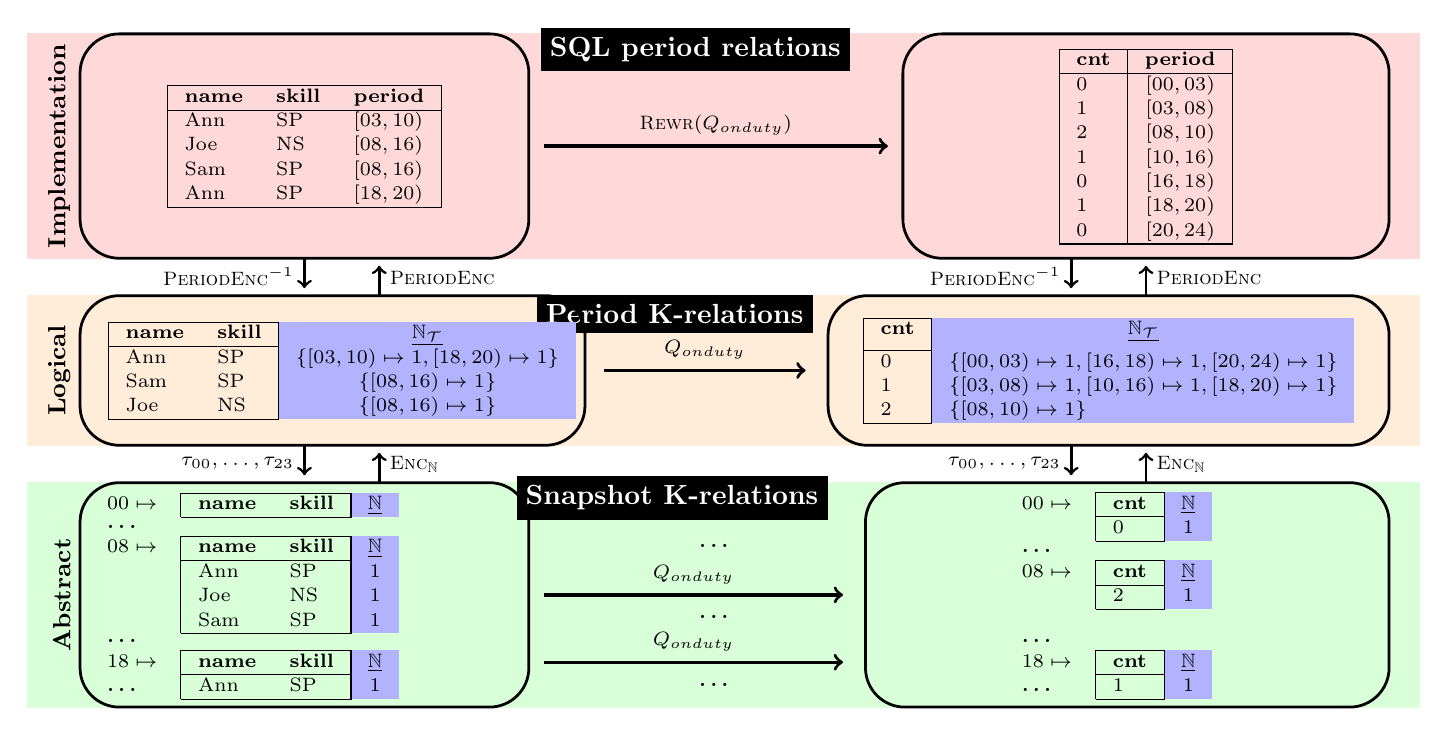
\begin{tikzpicture}[scale=0.95]


\newcommand{\ovfigLeftColumnWidth}{0.4\linewidth}
\newcommand{\ovfigMiddleColumnWidth}{0.09\linewidth}
\newcommand{\ovfigRightColumnWidth}{0.43\linewidth}



  \tikzstyle{every node}=[font=\scriptsize]
  {\renewcommand{\arraystretch}{1.1}

%%%%%%%%%%%%%%%%%%%%%%%%%%%%%%

 % \draw[rounded corners=0.1cm] (-0.7,3.2) rectangle (17.9,-6.2);

  \draw[fill=red!15,line width=0pt,color=red!15] (-0.7,3) rectangle (17.9,-0);
  \draw[fill=orange!15,line width=0pt,color=orange!15] (-0.7,-0.5) rectangle (17.9,-2.5);
  \draw[fill=green!15,line width=0pt,color=green!15] (-0.7,-3) rectangle (17.9,-6);

  \begin{scope}[shift={(0,0)}]

    \node[above, rotate=90] at (0,1.5) {{\bf \small Implementation}};
    \node[color=white, fill=black, above left] at (10.3,2.5) {{\normalsize \bf \SQLrels{}}};

    \draw [rounded corners=0.5cm, line width=1pt] (0,0) rectangle ++(6,3);
    \node at (3,1.5) {
      \begin{tabular}{|lll|}
			%\multicolumn{3}{l}{\textbf{works}} \\
			\cline{1-3}
			\thead{name} &\thead{skill} & \thead{period}\\
			\cline{1-3}
			Ann & SP & $[03, 10)$ \\
      Joe & NS & $[08, 16)$ \\
			Sam & SP & $[08, 16)$ \\
      Ann & SP & $[18, 20)$ \\
			\cline{1-3}
		  \end{tabular}
    };
    \draw[rounded corners=0.5cm, line width=1pt] (11,0) rectangle ++(6.5,3);
    \node at (14.25,1.5) {
  		\begin{tabular}{|l|c|}
  			\cline{1-2}
  			\thead{cnt} & \thead{period}\\
  			\cline{1-2}
  			0 & $[00, 03)$ \\
  			1 & $[03, 08)$ \\
  			2 & $[08, 10)$ \\
  			1 & $[10, 16)$ \\
  			0 & $[16, 18)$ \\
        1 & $[18, 20)$ \\
        0 & $[20, 24)$ \\
  			\cline{1-2}
  		\end{tabular}
    };
    \draw[->, very thick] (6.2,1.5) -- ++(4.6,0) node[pos=0.5, above] {$\reprRewr(Q_{onduty})$};
  \end{scope}


  \draw[->, line width=1pt] (3, 0) -- (3, -0.4) node[pos=0.6, left] {$\reprN^{-1}$};
  \draw[->, line width=1pt] (4, -0.5) -- (4, -0.1) node[pos=0.6, right] {$\reprN$};

  \draw[->, line width=1pt] (13.25, 0) -- (13.25, -0.4) node[pos=0.6, left] {$\reprN^{-1}$};
  \draw[->, line width=1pt] (14.25, -0.5) -- (14.25, -0.1) node[pos=0.6, right] {$\reprN$};

%%%%%%%%%%%%%%%%%%%%%%%%%%%%%%
  \begin{scope}[shift={(0,-3)}]

    \node[above, rotate=90] at (0,1.5) {{\bf \small Logical}};
    \node[color=white, fill=black, above left] at (9.8,2) {{\normalsize \bf Period K-relations}};

    \draw [rounded corners=0.5cm, line width=1pt] (0,0.5) rectangle ++(6.75,2);
    \node at (3.5,1.5) {
  		\begin{tabular}{|ll|c}
  			\cline{1-2}
  			\thead{name} &\thead{skill} & \annotheadcell{$\semTimeNIN$}\\
  			\cline{1-2}
  			Ann & SP & \annotcell{$\{[03, 10) \mapsto 1, [18,20) \mapsto 1\}$} \\
  			Sam & SP & \annotcell{$\{[08, 16) \mapsto 1 \}$} \\
  			Joe & NS & \annotcell{$\{[08, 16) \mapsto 1\}$} \\
  			\cline{1-2}
  		\end{tabular}
    };
    \draw[rounded corners=0.5cm, line width=1pt] (10,0.5) rectangle ++(7.5,2);
    \node at (13.75,1.5) {
  		\begin{tabular}{|l|l}
  			\cline{1-1}
  			\thead{cnt} & \multicolumn{1}{c}{\annotheadcell{$\semTimeNIN$}}\\[1mm]
  			\cline{1-1}
            0 & \annotcell{$\{ [00, 03) \mapsto 1, [16, 18) \mapsto 1,[20, 24) \mapsto 1 \}$} \\
            1 & \annotcell{$\{ [03, 08) \mapsto 1, [10, 16) \mapsto 1 ,[18, 20) \mapsto 1\}$} \\
  			    2 & \annotcell{$\{ [08, 10) \mapsto 1\}$} \\

            \cline{1-1}
  			\cline{1-1}
  		\end{tabular}
    };
    \draw[->, very thick] (7,1.5) -- ++(2.7,0) node[pos=0.5, above] {$Q_{onduty}$} ;
  \end{scope}

  \draw[->, line width=1pt] (3, -2.5) -- (3, -2.9) node[pos=0.6, left] {$\tSlice{00}, \ldots, \tSlice{23}$};
  \draw[->, line width=1pt] (4, -3) -- (4, -2.6) node[pos=0.6, right] {$\repr_{\semN}$};

  \draw[->, line width=1pt] (13.25, -2.5) -- (13.25, -2.9) node[pos=0.6, left] {$\tSlice{00}, \ldots, \tSlice{23}$};
  \draw[->, line width=1pt] (14.25, -3) -- (14.25, -2.6) node[pos=0.6, right] {$\repr_{\semN}$};

  %%%%%%%%%%%%%%%%%%%%%%%%%%%%%%
    \begin{scope}[shift={(0,-6)}]

      \node[above, rotate=90] at (0,1.5) {{\bf \small \revc{Abstract}}};
      \node[color=white,fill=black, above left] at (10,2.5) {{\normalsize \bf Snapshot K-relations}};

      \draw [ rounded corners=0.5cm, line width=1pt] (0,0) rectangle ++(6,3);
      \node at (2.2,2.7) {
        \begin{tabular}{l|ll|c}
          \cline{2-3}
           $00 \mapsto {}$ & \thead{name} &\thead{skill} &  \annotheadcell{$\semN$}\\
          \cline{2-3}
        \end{tabular}
      };
      \node at (2.2,1.8) {
        \begin{tabular}[t]{l|ll|c}
          \multicolumn{2}{l}{{\bf \ldots}} & \multicolumn{1}{l}{} &\\
          \cline{2-3}
           $08 \mapsto {}$ & \thead{name} &\thead{skill} &  \annotheadcell{$\semN$}\\
           \cline{2-3}
           & Ann & SP & \annotcell{1} \\
           & Joe & NS & \annotcell{1} \\
           & Sam & SP & \annotcell{1} \\
          \cline{2-3}
        \end{tabular}
      };
      \node at (2.2,0.6) {
        \begin{tabular}[t]{l|ll|c}
          \multicolumn{2}{l}{{\bf \ldots}} & \multicolumn{1}{l}{} &\\
          \cline{2-3}
           $18 \mapsto {}$ & \thead{name} &\thead{skill} &  \annotheadcell{$\semN$}\\
           \cline{2-3}
           \multicolumn{1}{l|}{{\bf \ldots}} & Ann & SP & \annotcell{1} \\
          \cline{2-3}
        \end{tabular}
      };

      \draw[rounded corners=0.5cm, line width=1pt] (10.5,0) rectangle ++(7,3);
      \node at (13.75,2.55) {
        \begin{tabular}{l|l|c}
          \cline{2-2}
           $00 \mapsto {}$ & \thead{cnt} &  \annotheadcell{$\semN$}\\
           \cline{2-2}
            & 0 & \annotcell{1} \\
          \cline{2-2}
        \end{tabular}
      };
      \node at (13.75,1.8) {
        \begin{tabular}{l|l|c}
          \multicolumn{2}{l}{{\bf \ldots}} & \multicolumn{1}{l}{}\\
          \cline{2-2}
           $08 \mapsto {}$ & \thead{cnt} &  \annotheadcell{$\semN$}\\
           \cline{2-2}
            & 2 & \annotcell{1} \\
          \cline{2-2}
        \end{tabular}
      };
      \node at (13.75,0.6) {
        \begin{tabular}{l|l|c}
          \multicolumn{2}{l}{{\bf \ldots}} & \multicolumn{1}{l}{}\\
          \cline{2-2}
           $18 \mapsto {}$ & \thead{cnt} &  \annotheadcell{$\semN$}\\
           \cline{2-2}
            {\bf \ldots}& 1 & \annotcell{1} \\
          \cline{2-2}
        \end{tabular}
      };
      % \draw[->, very thick] (7.2,2.5) -- ++(2.6,0) node[pos=0.5, above] {$Q_{onduty}
      % %(\tSlice{00}(\textbf{works}))
      % $} ;
      \node at (8.5, 2.15) {{\bf \ldots}};
      \draw[->, very thick] (6.2,1.5) -- ++(4,0) node[pos=0.5, above] {$Q_{onduty}
      %(\tSlice{08}(\textbf{works}))
      $} ;
      \node at (8.5, 1.2) {{\bf \ldots}};
      \draw[->, very thick] (6.2,0.6) -- ++(4,0) node[pos=0.5, above] {$Q_{onduty}
      %(\tSlice{18}(\textbf{works}))
      $} ;
      \node at (8.5, 0.3) {{\bf \ldots}};
    \end{scope}

  }

  \end{tikzpicture}
  \caption{Overview of our approach. Our \emph{\revc{abstract} model} is
  \emph{snapshot K-relations} and nontemporal queries over snapshots (snapshot semantics). Our
  \emph{logical} model is \emph{period K-relations} and % temporal
  queries
  corresponding to the \reva{abstract} model's snapshot queries. % in the \revc{abstract} model.
  Our
  \emph{implementation} uses \emph{\SQLrels{}} and
  rewritten non-temporal queries implementing the other model's snapshot queries. % of the two other models.
  Each model is associated with
  transformations to the other models % below and above
  which commute with queries (modulo the rewriting $\reprRewr$ when mapping to the implementation). % As we will demonstrate, all of these transformations commute with queries (modulo the rewriting $\reprRewr$ when translating from the logical model to the implementation).
} % e.g., for any period K-database $D$, query $Q$, and timepoint $\tPoint$ we have $\query(\tSlice{\tPoint}(D)) = \tSlice{\tPoint}(\query(D))$, which is \emph{snapshot-reducibility}.}
  \label{fig:overview-approach}
\end{figure*}

%%% Local Variables:
%%% mode: latex
%%% TeX-master: "../pvldb.tex"
%%% End:

%
%
% %%%%%%%%%%%%%%%%%%%%%%%%%%%%%%%%%%%%%%%%%%%%%%%%%%%%%%%%%%%%%%%%%%%%%%%%%%%%%%%%
% % non-sequenced languages
% \parttitle{Non-sequenced Temporal Queries}
% Non-sequenced temporal query languages, such as
% IXSQL~\cite{LorentzosM97} and SQL/TP~\cite{T98}, do not explicitly
% support sequenced semantics.
% % Hence, a comparison to the approaches in
% % Table~\ref{tab:table-rel-work-bugs} is meaningless.
% Nevertheless, we review these languages here since they allow to
% express queries with sequenced semantics.
% %
% % \revdel{IXSQL~\cite{LorentzosM97} introduces several interval-specific
% % conditions (e.g., checking for overlap) and two operations, fold and
% % unfold, that translate between point-based and interval-based
% % representations of temporal data. The language essentially treats
% % temporal attributes as regular data. To write a temporal query, the
% % user has to combine (un)fold, regular non-temporal algebra
% % operators, and the new temporal conditional constructs.}
% %
% % \revdel{SQL/TP~\cite{T98} introduces a point-wise semantics for temporal
% % queries~\cite{BowmanT03,T96}. Time is handled as a regular attribute
% % with the exception that relations can be infinite in the time
% % dimension. The language supports multiset semantics.  Intervals are
% % used as an efficient encoding of time points, and a normalization
% % operation is used to split intervals. The interval-based encoding of
% % the language is not unique, since time points are grouped into
% % intervals based on query syntax and based on how the input is encoded
% % as period relations.  While this has no effect on the semantics since
% % SQL/TP queries cannot distinguish between different interval-based
% % encodings of a temporal database, it might be confusing to users that
% % observe different query results for equivalent queries/inputs.}
% \revc{SQL/TP~\cite{T98} introduces a point-wise semantics for temporal
% queries~\cite{BowmanT03,T96}, where time is handled as a regular attribute.
% Intervals are used as an efficient encoding of time points, and a normalization
% operation is used to split intervals. The language supports multisets and a
% mechanism to manually produce sequenced semantics. However, sequenced semantics queries are specified as the union of non-temporal queries over snapshots. Even if such subqueries are grouped together for adjacent time points where the non-temporal query's result is constant this still results in a large number of subqueries to be executed. Even worse, the number of subqueries that is required is data dependent.
% % but is subject to the
% % \abbrAGB{} bug.
% Also, the interval-based encoding is not unique, since time
% points are grouped into intervals depending on query syntax and encoding of the
% input. While this has no effect on the semantics since SQL/TP queries cannot
% distinguish between different interval-based encodings of a temporal database,
% it might be confusing to users that observe different query results for
% equivalent queries/inputs.}
%
% %%%%%%%%%%%%%%%%%%%%
% %\revdel{
% \parttitle{Implementations of Temporal Operators}
% %
% A large body of work has focused on the implementation of individual
% temporal algebra operators such as
% joins~\cite{DBLP:conf/sigmod/DignosBG14,DBLP:conf/icde/PiatovHD16,DBLP:journals/pvldb/BourosM17}
% and
% aggregation~\cite{DBLP:conf/edbt/BohlenGJ06,DBLP:conf/sigmod/PilmanKKKP16,DBLP:conf/ssd/PiatovH17}. Some
% exceptions supporting multiple operators
% are~\cite{DBLP:conf/sigmod/KaufmannMVFKFM13, DignosBGJ16,
%   CafagnaB17}. These approaches introduce efficient evaluation
% algorithms for a particular semantics of a temporal algebra operator.
% Our approach can utilize efficient operator implementations as long as
% (i) their semantics is compatible with our interval-based encoding of
% snapshot query results and (ii) they are snapshot-reducible.
% %}
%
%  %%%%%%%%%%%%%%%%%%%%%%%%%%%%%%%%%%%%%%%%
% \parttitle{Coalescing}
% %
% Coalescing produces a unique representation of a \emph{set} semantics
% temporal database.  B\"ohlen et al.~\cite{DBLP:conf/vldb/BohlenSS96}
% study optimizations for coalescing % and present % algebraic
% % rewrites that
% that eliminate unnecessary coalescing operations. Zhou et
% al.~\cite{ZhouWZ06} and~\cite{DBLP:conf/dexa/Al-KatebGC12} use analytical functions to efficiently
% implement coalescing in SQL.
% %
% We generalize coalescing to $\semK$-relations % and apply the resulting
% % operation, which we call $\semK$-coalescing,
% to define a unique encoding of
% interval-based temporal relations, including \emph{multiset} relations. Similar
% to~\cite{DBLP:conf/vldb/BohlenSS96}, we remove unnecessary K-coalescing steps
% and, similar to~\cite{ZhouWZ06}, we use OLAP functions for efficient implementation.
% %$\semK$-coalescing.
%
% \BGDel{Our approach is guided by providing a clean framework that is
%   able to generally define all operators under different data model
%   semantics, such as set and multiset semantics. This framework is
%   crucial to categorize existing implementations, but also to generate
%   new ones for cases where no existing is available, such as for
%   example multiset difference.}
%
%
%
% \parttitle{Temporality in Annotated Databases}
% %
% Kostiley et al.~\cite{KB12} is to the best of our knowledge the only
% previous approach that uses semiring annotations to express
% temporality. The authors define a semiring whose elements are sets of
% time points. This approach is limited to set semantics, and no
% % efficient
% interval-based encoding was presented.  The LIVE
% system~\cite{DT10} combines provenance and uncertainty annotations
% with versioning. The system uses interval timestamps, and query
% semantics is based on snapshot-reducibility~\cite[Def.\
% 2]{DT10}. However, computing the intervals associated with a query
% result requires provenance % (semiring $PosBool(X)$)
% to be maintained for every query result.

%%%%%%%%%%%%%%%%%%%%%%%%%%%%%%%%%%%%%%%%%%%%%%%%%%%%%%%%%%%%%%%%%%%%%%%%%%%%%%%%
\section{Related Work}
\label{sec:related-work}
%%%%%%%%%%%%%%%%%%%%%%%%%%%%%%%%%%%%%%%%%%%%%%%%%%%%%%%%%%%%%%%%%%%%%%%%%%%%%%%%

%%%%%%%%%%%%%%%%%%%%
\parttitle{Temporal Query Languages}
%
There is a long history of research on temporal query
languages~\cite{DBLP:reference/db/JensenS09r,DBLP:reference/db/BohlenGJS09}.
Many temporal query languages including
TSQL2~\cite{Snodgrass95,DBLP:journals/sigmod/SnodgrassAABCDEGJKKKLLRSSS94},
\mbox{ATSQL2} (Applied TSQL2)~\cite{Bohlen95evaluatingand},
IXSQL~\cite{LorentzosM97}, ATSQL~\cite{BohlenJS00}, and
SQL/TP~\cite{T98} support snapshot semantics.  In this paper, % we do
% not focus on a particular query language. Rather,
we provide a general
framework that can be used to correctly implement snapshot semantics
over period set and multiset relations for any language.

%%%%%%%%%%%%%%%%%%%%
\parttitle{Interval-based Approaches for Snapshot Semantics}
In the following, we discuss interval-based approaches for snapshot
semantics.
%
Table~\ref{tab:table-rel-work-bugs} shows for each approach whether it
supports multisets, whether it is free of the aggregation gap and bag
difference bugs, and whether its interval-based encoding of a
snapshot query result is unique. An N/A indicates that the approach
does not support the operation for which this type of bug can occur or
the semantics of this operation is not defined precisely enough to
judge its correctness.  Note that while temporal query languages may
be defined to apply snapshot semantics and, thus, by definition are
snapshot-reducible, (the specification of) their implementation might
fail to be snapshot-reducible.  In the following discussion of the
temporal query languages in Table~\ref{tab:table-rel-work-bugs}, we
refer to their semantics as provided in the referenced publication(s).

%%%%%%%%%%%%%%%%%%%%
% Interval preservation
\emph{Interval preservation} (ATSQL)~\cite[Def.\ 2.10]{BohlenJS00} is a
representation system for SQL period relations (multisets) that tries to
preserve
the intervals associated with input
tuples, i.e., fragments of all intervals (including duplicates)
associated with the input tuples ``survive'' in the output.  Interval
preservation is snapshot-reducible for multiset semantics for positive
relational algebra\revc{\cite{DBLP:reference/db/Sirangelo09c} (selection, projection, join, and union)}, but exhibits the aggregation gap and bag difference
bug.  Moreover, the period encoding of a query result is not unique as
it depends both on the query and the input representation.
%
%%%%%%%%%%%%%%%%%%%%
% Teradata
\emph{Teradata}~\cite{teradata1510} is a commercial DBMS that supports
snapshot operators using ATSQL's statement modifiers. The
implementation is based on query
rewriting~\cite{DBLP:conf/edbt/Al-KatebGCBCP13} and does not support
difference.  Teradata's implementation exhibits the aggregation gap
bug. Since the application of coalescing is optional, the encoding of
snapshot relations as period relations is not unique.
%
%%%%%%%%%%%%%%%%%%%%
% Change preservation
% \revdel{\emph{Change preservation}~\cite[Def.\ 3.4]{DignosBGJ16} determines
% the interval boundaries of a query result tuple $\tuple$ based on the
% intervals attached to tuples in $\tuple$'s provenance. Whether such an
% encoding of a result is unique for equivalent queries depends on the
% provenance model that is employed. If the provenance model is
% insensitive to query rewrite~\cite{CC09}, i.e., equivalent queries
% have the same provenance, then the corresponding change-preservation
% encoding is unique for a given interval-timestamped input relation
% (but not necessarily for different snapshot-equivalent inputs).
% Change preservation was originally studied for set semantics employing
% the lineage provenance model in~\cite{DignosBG12} and the PI-CS model
% in~\cite{DignosBGJ16} (which for positive queries is equivalent to
% provenance polynomials in the semiring annotation
% framework~\cite{GM13}). However, none of the two models has the same
% equivalences as set semantics (the correct choice would be semiring
% PosBool(X)~\cite{GK07,G09} aka Minimal Why-provenance~\cite{CC09}).}
\revc{\emph{Change preservation}~\cite[Def.\ 3.4]{DignosBGJ16} determines the
interval boundaries of a query result tuple $\tuple$ based on the maximal
interval for which there is no change in the input, i.e., sequenced semantics. To track changes, it
employs the lineage provenance model in~\cite{DignosBG12} and the PI-CS model
in~\cite{DignosBGJ16}.
The approach
uses timestamp adjustment in combination with traditional database operators, but does not provide a unique encoding, exhibits the AG bug,
and only supports set semantics. Our work solves the AG bug. Furthermore, we provide a unique encoding and support bag semantics in addition to set semantics.}
%
%%%%%%%%%%%%%%%%%%%%
%TSQL2
% \emph{TSQL2}~\cite{Snodgrass95,DBLP:journals/sigmod/SnodgrassAABCDEGJKKKLLRSSS94}
% applies coalescing~\cite{DBLP:conf/vldb/BohlenSS96} implicitly and,
% thus, only supports set semantics. Soo et al.~\cite{SJ95} introduced a
% temporal algebra to formalize TSQL2's semantics. This algebra is
% set-based and uses coalescing to produce a unique representation. This
% algebra does not include aggregation.
\emph{TSQL2}~\cite{Snodgrass95,DBLP:journals/sigmod/SnodgrassAABCDEGJKKKLLRSSS94,SJ95}
implicitly applies coalescing~\cite{DBLP:conf/vldb/BohlenSS96} to
produce a unique representation. Thus, it only supports  set semantics,
and it does not support aggregation.
%
%%%%%%%%%%%%%%%%%%%%
% Adding Validtime to SQL/temporal
Snodgrass et al.~\cite{SB96} present a validtime extension of
\emph{SQL/Temporal} and an algebra with snapshot semantics. The
algebra supports multisets, but exhibits both the aggregation gap and
bag difference bug. Since intervals from the input are preserved
where possible, the interval representation of a snapshot
relation is not unique.
%
%%%%%%%%%%%%%%%%%%%%
% TimeDB
\emph{TimeDB}~\cite{S98} is an implementation of
ATSQL2~\cite{Bohlen95evaluatingand}. It uses a semantics for bag
difference and intersection that is not snapshot-reducible
(see~\cite[pp.\ 63]{S98}).
%
%%%%%%%%%%%%%%%%%%%%
% Our approach
 Our approach is the first that supports set and multiset relations,
 is resilient against the two bugs, and specifies a unique
 interval-encoding. % for the implementation.


%%%%%%%%%%%%%%%%%%%%%%%%%%%%%%%%%%%%%%%%
\begin{table}[tb]
  \caption{Interval-based approaches for snapshot semantics.}
  \label{tab:table-rel-work-bugs}

  \centering
  \small

  \newcommand{\bugtableheaderheight}{1.2cm}
  \renewcommand{\arraystretch}{1.1}

  \begin{tabular}{|l|c|c|c|c|}
    \hline
    \thead{Approach}
    & \thead{
      \rotatebox{90}{
      \begin{minipage}{\bugtableheaderheight}
        Multisets
      \end{minipage}
      }
      }
    & \thead{
      \rotatebox{90}{
      \begin{minipage}{\bugtableheaderheight}
        \abbrAGB{} bug\\ free
      \end{minipage}
      }
      }
    & \thead{
      \rotatebox{90}{
      \begin{minipage}{\bugtableheaderheight}
        \abbrBDB{} bug\\ free
      \end{minipage}
      }
      }
    & \thead{
      \rotatebox{90}{
      \begin{minipage}{\bugtableheaderheight}
        Unique \\ encoding
      \end{minipage}
    }
    }
    \\
    \hline
    Interval preservation~\cite{BohlenJS00} (ATSQL) & \checkmark & $\times$ & $\times$ & $\times$
    \\
    Teradata~\cite{teradata1510} & \checkmark & $\times$ & N/A  & $\times$\tablefootnote{Optionally, coalescing (\texttt{NORMALIZE ON} in Teradata) can be applied to get a unique encoding at the cost of loosing multiplicities.}
    \\
    Change preservation~\cite{DignosBG12,DignosBGJ16} & $\times$ & $\times$& N/A & $\times$
    \\
    TSQL2~\cite{Snodgrass95,DBLP:journals/sigmod/SnodgrassAABCDEGJKKKLLRSSS94,SJ95} & $\times$ & N/A & N/A & $\checkmark$
    \\
    ATSQL2~\cite{Bohlen95evaluatingand} & \checkmark & N/A & $\times$ & $\times$
    \\
    TimeDB~\cite{S98} (ATSQL2) & \checkmark & N/A & $\times$& $\times$
    \\
    SQL/Temporal~\cite{SB96} & \checkmark & $\times$ & $\times$ & $\times$
    \\
    \revc{SQL/TP~\cite{T98}\tablefootnote{Snapshot semantics can be expressed, but this is inefficient.}} & \revc{\checkmark{}} & \revc{\checkmark{}} & \revc{\checkmark{}} & \revc{$\times$}
    \\
    {\bf Our approach} & \checkmark & \bf \checkmark & \checkmark & \checkmark
    \\
    \hline
  \end{tabular}
\end{table}
%%%%%%%%%%%%%%%%%%%%%%%%%%%%%%%%%%%%%%%%
% Overview figure is placed here in order to appear on top of Sec. 3
%!TEX root = ../document.tex

% %%%%%%%%%%%%%%%%%%%%%%%%%%%%%%%%%%%%%%%%%%%%%%%%%%%%%%%%%%%%%%%%%%%%%%%%%%%%%%%%
% \begin{figure*}[t]
%   \centering


% %%%%%%%%%%%%%%%%%%%%%%%%%%%%%%%%%%%%%%%%
%   \begin{minipage}{\ovfigLeftColumnWidth}
%     \centering
%         \footnotesize
% 		\begin{tabular}{|ll|l|}
% 			\multicolumn{3}{c}{\textbf{works}} \\
% 			\cline{1-3}
% 			\thead{name} &\thead{skill} & \thead{period}\\
% 			\cline{1-3}
% 			Ann & SP & $[1, 7)$ \\
% 			Sam & SP & $[5, 11)$ \\
% 			Ann & SP & $[13, 14)$ \\
% 			Joe & NS & $[3, 12)$ \\
% 			\cline{1-3}
% 		\end{tabular}
%   \end{minipage}
%   \begin{minipage}{\ovfigMiddleColumnWidth}
%     \centering
%     {$\reprRewr(Q_{spOnDuty})$}\\[2mm]
%     \myrightarrow
%   \end{minipage}
%   \begin{minipage}{\ovfigRightColumnWidth}
%     \centering
%         \footnotesize
% 		\begin{tabular}{|l|c|}
% 			\cline{1-2}
% 			\thead{cnt} & \thead{period}\\
% 			\cline{1-2}
% 			0 & $[-\infty, 1)$ \\
% 			1 & $[1, 5)$ \\
% 			2 & $[5, 7)$ \\
% 			1 & $[7, 11)$ \\
% 			0 & $[11, 13)$ \\
% 			1 & $[13, 14)$ \\
% 			0 & $[14, \infty)$ \\
% 			\cline{1-2}
% 		\end{tabular}

%   \end{minipage}
% %%%%%%%%%%%%%%%%%%%%%%%%%%%%%%%%%%%%%%%%

% %%%%%%%%%%%%%%%%%%%%%%%%%%%%%%%%%%%%%%%%
%   \begin{minipage}{\ovfigLeftColumnWidth}
%     \centering
% {\footnotesize $\reprN^{-1}$} \mydownarrow \hspace{1cm}\myuparrow {\footnotesize $\reprN$}
%   \end{minipage}
%   \begin{minipage}{\ovfigMiddleColumnWidth}
%     \centering
%     \mydownarrow {\footnotesize \reprRewr}
%   \end{minipage}
%   \begin{minipage}{\ovfigRightColumnWidth}
%    \centering
% {\footnotesize $\reprN^{-1}$} \mydownarrow \hspace{1cm}\myuparrow {\footnotesize $\reprN$}
%   \end{minipage}
% %%%%%%%%%%%%%%%%%%%%%%%%%%%%%%%%%%%%%%%%

% %%%%%%%%%%%%%%%%%%%%%%%%%%%%%%%%%%%%%%%%
%   \begin{minipage}{\ovfigLeftColumnWidth}
%     \centering
%         \footnotesize
% 		\begin{tabular}{|ll|l}
% 			\multicolumn{2}{c}{\textbf{works}} \\
% 			\cline{1-2}
% 			\thead{name} &\thead{skill} & \annotheadcell{$\semTimeNIN$}\\
% 			\cline{1-2}
% 			Ann & SP & \annotcell{$\{[1, 7) \mapsto 1, [13,14) \mapsto 1\}$} \\
% 			Sam & SP & \annotcell{$\{[5, 11) \mapsto 1 \}$} \\
% 			Joe & NS & \annotcell{$\{[3, 12) \mapsto 1\}$} \\
% 			\cline{1-2}
% 		\end{tabular}
%       \end{minipage}
%   \begin{minipage}{\ovfigMiddleColumnWidth}
%     \centering
%         {$Q_{spOnDuty}$}\\[2mm]
%     \myrightarrow
%   \end{minipage}
%   \begin{minipage}{\ovfigRightColumnWidth}
%         \footnotesize
% 		\begin{tabular}{|l|l}
% 			\cline{1-1}
% 			\thead{cnt} & \multicolumn{1}{c}{\annotheadcell{$\semTimeNIN$}}\\[1mm]
% 			\cline{1-1}
%           0 & \annotcell{$\{ [-\infty, 1) \mapsto 1, [11, 13) \mapsto 1,[14, \infty) \mapsto 1 \}$} \\
%           1 & \annotcell{$\{ [1, 5) \mapsto 1, [7, 11) \mapsto 1, [13, 14) \mapsto 1\}$} \\
% 			2 & \annotcell{$\{ [5, 7) \mapsto 1 \}$} \\ \cline{1-1}
% 			\cline{1-1}
% 		\end{tabular}  \end{minipage}
% %%%%%%%%%%%%%%%%%%%%%%%%%%%%%%%%%%%%%%%%


% %%%%%%%%%%%%%%%%%%%%%%%%%%%%%%%%%%%%%%%%
%   \begin{minipage}{\ovfigLeftColumnWidth}
%     \centering
%  \myuparrow {\footnotesize $\repr_{\semN}$}
%   \end{minipage}
%   \begin{minipage}{\ovfigMiddleColumnWidth}
%     \centering
%   \end{minipage}
%   \begin{minipage}{\ovfigRightColumnWidth}
%    \centering
%     \myuparrow {\footnotesize $\repr_{\semN}$}
%   \end{minipage}
% %%%%%%%%%%%%%%%%%%%%%%%%%%%%%%%%%%%%%%%%



% %%%%%%%%%%%%%%%%%%%%
%  \begin{minipage}{\ovfigLeftColumnWidth}
%     \centering
%         \tiny
%     \begin{minipage}{.49\linewidth}
%       $1 \mapsto{}$
%       		\begin{tabular}{|ll|c}
% 			\multicolumn{2}{c}{\textbf{works}} &\\
% 			\cline{1-2}
% 			\thead{name} &\thead{skill} &  \annotheadcell{$\semN$}\\
% 			\cline{1-2}
% 			Ann & SP & \annotcell{1} \\
% 			\cline{1-2}
% 		\end{tabular}
%     \end{minipage}
%     \hfill
%     \begin{minipage}{.49\linewidth}
%       $2 \mapsto{}$
%       		\begin{tabular}{|ll|c}
% 			\multicolumn{2}{c}{\textbf{works}} & \\
% 			\cline{1-2}
% 			\thead{name} &\thead{skill} &  \annotheadcell{$\semN$}\\
% 			\cline{1-2}
%               Ann & SP & \annotcell{1}\\
% 			\cline{1-2}
%             \end{tabular}
%     \end{minipage}
%     \hfill
%     \begin{minipage}{.49\linewidth}
%       $3 \mapsto{}$
%       \begin{tabular}{|ll|c}
% 			\multicolumn{2}{c}{\textbf{works}} & \\
% 			\cline{1-2}
% 			\thead{name} &\thead{skill} &  \annotheadcell{$\semN$} \\
% 			\cline{1-2}
% 			Ann & SP & \annotcell{1} \\
%             Joe & NS & \annotcell{1}\\
%             \cline{1-2}
% 	  \end{tabular}
%     \end{minipage}
%     \begin{minipage}{0.49\linewidth}
%       \center
%       {\Large \ldots}
%     \end{minipage}
%   \end{minipage}
% %%%%%%%%%%%%%%%%%%%%
%   \begin{minipage}{\ovfigMiddleColumnWidth}
%     \centering
%     {$Q_{spOnDuty}$}\\[2mm]
%     \myrightarrow
%   \end{minipage}
% %%%%%%%%%%%%%%%%%%%%
%   \begin{minipage}{\ovfigRightColumnWidth}
%     \centering
%         \tiny
%     \begin{minipage}{.29\linewidth}
%       $1 \mapsto{}$
% \begin{tabular}{|l|c}
% 			\cline{1-1}
% 			\thead{cnt} &   \annotheadcell{$\semN$}\\
% 			\cline{1-1}
% 			1  & \annotcell{1}\\
% 			\cline{1-1}
% 		\end{tabular}
%     \end{minipage}
%     \hfill
%     \begin{minipage}{0.1\linewidth}
%       {\Large \ldots}
%     \end{minipage}
%     \hfill
%     \begin{minipage}{.29\linewidth}
%       $5 \mapsto{}$
% \begin{tabular}{|l|c}
% 			\cline{1-1}
% 			\thead{cnt} &   \annotheadcell{$\semN$}\\
% 			\cline{1-1}
% 			2  & \annotcell{1}\\
% 			\cline{1-1}
% 		\end{tabular}
%     \end{minipage}
%     \hfill
%     \begin{minipage}{0.1\linewidth}
%       {\Large \ldots}
%     \end{minipage}
%    \end{minipage}\\[3mm]

%   \caption{Our approach for snapshot semantics queries over multiset relations: 1) we define relations annotated with temporal $\semN$-elements, functions that map  intervals to multiplicities, define a query semantics over such relations and prove that they are a representation system for snapshot multiset relations (they correctly implement snapshot semantics over mutltiset relations); 2) we demonstrate how this semantics can be implemented as SQL queries over an encoding of temporal information as  interval-timestamped tuples.}
%   \label{fig:approach-overview}
% \end{figure*}
% %%%%%%%%%%%%%%%%%%%%%%%%%%%%%%%%%%%%%%%%%%%%%%%%%%%%%%%%%%%%%%%%%%%%%%%%%%%%%%%%

% \begin{figure}
%   \begin{tikzpicture}[scale=.4]
%   \tikzstyle{every node}=[font=\scriptsize]
%
%   \coordinate (A) at (1,0);
%   \coordinate (B) at ($(1,0)+(20,0)+(.7cm,0)$);
%
%   \draw[->,very thick] (A)--(B);
%   \foreach \t/\m in {1,2,3,4,5,6,7,8,9,10,11,12,13,14,15,16,17,18,19,20}
%   {
%     \draw[very thick] (\t cm,-1mm)--(\t cm,1mm);
%     \draw ($(\t cm,0)+(.5cm,0)$)
%     node[below, font=\fontsize{6}{6}\selectfont]{\m};
%   }
%   \draw[very thick] ($(B)+(-.7cm,-1mm)$)--($(B)+(-.7cm,1mm)$);
%   \draw ($(B)+(-.5mm,-.5mm)$) node[below]{$h$};
%
%   \begin{scope}[shift={(2,0)}]
%
%     \draw[thick] (1,4.9)--+(9,0) node[pos=.5,above=-2pt]{M1, SP};
%     \draw[thick] (4,4.1)--+(8,0) node[pos=.5,above=-2pt]{M2, SP};
%     \draw[thick] (1,3.3)--+(13,0) node[pos=.5,above=-2pt]{M3, NS};
%
%
%     \draw[thick] (1,2.1)--+(7,0) node[pos=.5,above=-2pt]{Ann, SP};
%     \draw[thick] (6,1.3)--+(8,0) node[pos=.5,above=-2pt]{Sam, SP};
%     \draw[thick] (16,1.3)--+(2,0) node[pos=.5,above=-2pt]{Ann, SP};
%     \draw[thick] (6,0.5)--+(8,0) node[pos=.5,above=-2pt]{Joe, NS};
%   \end{scope}
%
%   \end{tikzpicture}
%   \caption{NEW EXAMPLE with hours 0-23 (to be dropped) only for us}
% \end{figure}

%%%%%%%%%%%%%%%%%%%%%%%%%%%%%%%%%%%%%%%%%%%%%%%%%%%%%%%%%%%%%%%%%%%%%%%%%%%%%%%%
\begin{figure*}[htb]
  \centering
  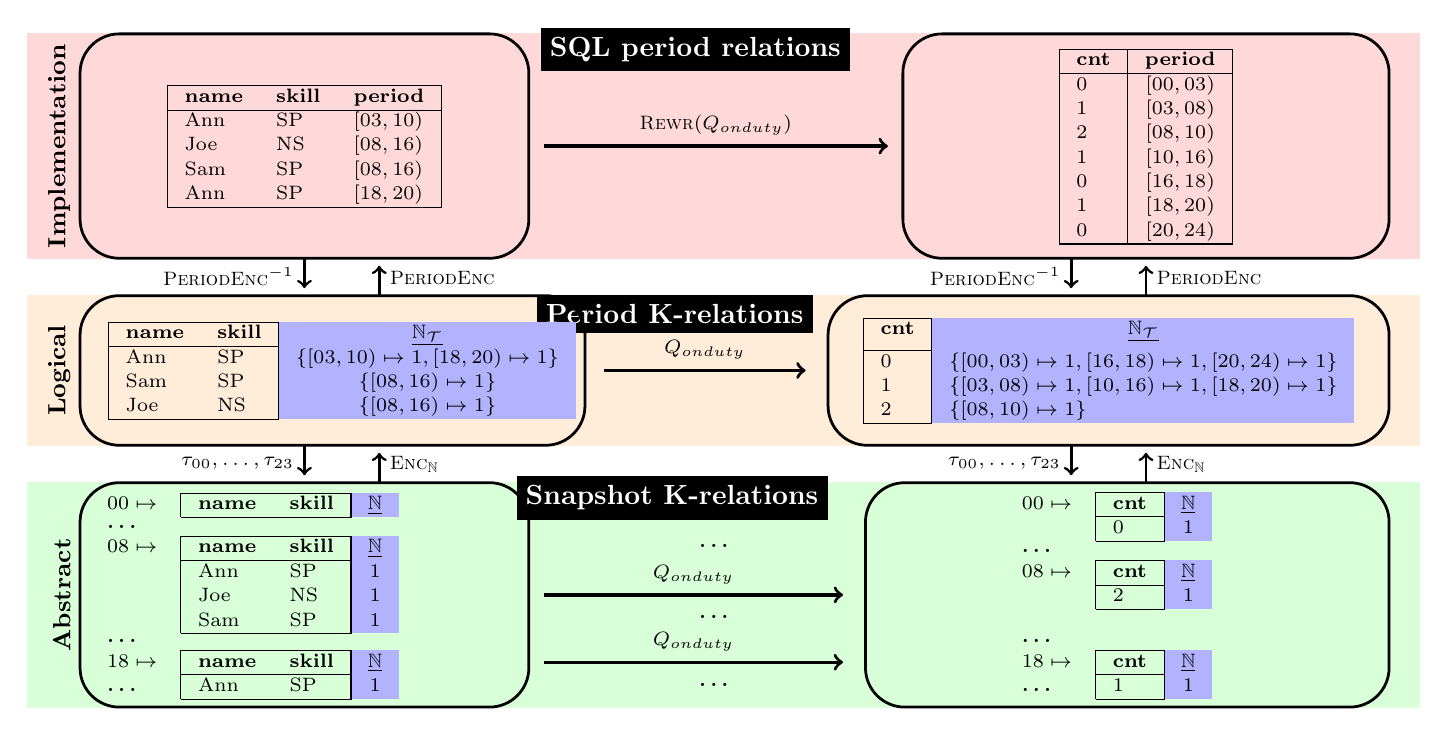
\begin{tikzpicture}[scale=0.95]


\newcommand{\ovfigLeftColumnWidth}{0.4\linewidth}
\newcommand{\ovfigMiddleColumnWidth}{0.09\linewidth}
\newcommand{\ovfigRightColumnWidth}{0.43\linewidth}



  \tikzstyle{every node}=[font=\scriptsize]
  {\renewcommand{\arraystretch}{1.1}

%%%%%%%%%%%%%%%%%%%%%%%%%%%%%%

 % \draw[rounded corners=0.1cm] (-0.7,3.2) rectangle (17.9,-6.2);

  \draw[fill=red!15,line width=0pt,color=red!15] (-0.7,3) rectangle (17.9,-0);
  \draw[fill=orange!15,line width=0pt,color=orange!15] (-0.7,-0.5) rectangle (17.9,-2.5);
  \draw[fill=green!15,line width=0pt,color=green!15] (-0.7,-3) rectangle (17.9,-6);

  \begin{scope}[shift={(0,0)}]

    \node[above, rotate=90] at (0,1.5) {{\bf \small Implementation}};
    \node[color=white, fill=black, above left] at (10.3,2.5) {{\normalsize \bf \SQLrels{}}};

    \draw [rounded corners=0.5cm, line width=1pt] (0,0) rectangle ++(6,3);
    \node at (3,1.5) {
      \begin{tabular}{|lll|}
			%\multicolumn{3}{l}{\textbf{works}} \\
			\cline{1-3}
			\thead{name} &\thead{skill} & \thead{period}\\
			\cline{1-3}
			Ann & SP & $[03, 10)$ \\
      Joe & NS & $[08, 16)$ \\
			Sam & SP & $[08, 16)$ \\
      Ann & SP & $[18, 20)$ \\
			\cline{1-3}
		  \end{tabular}
    };
    \draw[rounded corners=0.5cm, line width=1pt] (11,0) rectangle ++(6.5,3);
    \node at (14.25,1.5) {
  		\begin{tabular}{|l|c|}
  			\cline{1-2}
  			\thead{cnt} & \thead{period}\\
  			\cline{1-2}
  			0 & $[00, 03)$ \\
  			1 & $[03, 08)$ \\
  			2 & $[08, 10)$ \\
  			1 & $[10, 16)$ \\
  			0 & $[16, 18)$ \\
        1 & $[18, 20)$ \\
        0 & $[20, 24)$ \\
  			\cline{1-2}
  		\end{tabular}
    };
    \draw[->, very thick] (6.2,1.5) -- ++(4.6,0) node[pos=0.5, above] {$\reprRewr(Q_{onduty})$};
  \end{scope}


  \draw[->, line width=1pt] (3, 0) -- (3, -0.4) node[pos=0.6, left] {$\reprN^{-1}$};
  \draw[->, line width=1pt] (4, -0.5) -- (4, -0.1) node[pos=0.6, right] {$\reprN$};

  \draw[->, line width=1pt] (13.25, 0) -- (13.25, -0.4) node[pos=0.6, left] {$\reprN^{-1}$};
  \draw[->, line width=1pt] (14.25, -0.5) -- (14.25, -0.1) node[pos=0.6, right] {$\reprN$};

%%%%%%%%%%%%%%%%%%%%%%%%%%%%%%
  \begin{scope}[shift={(0,-3)}]

    \node[above, rotate=90] at (0,1.5) {{\bf \small Logical}};
    \node[color=white, fill=black, above left] at (9.8,2) {{\normalsize \bf Period K-relations}};

    \draw [rounded corners=0.5cm, line width=1pt] (0,0.5) rectangle ++(6.75,2);
    \node at (3.5,1.5) {
  		\begin{tabular}{|ll|c}
  			\cline{1-2}
  			\thead{name} &\thead{skill} & \annotheadcell{$\semTimeNIN$}\\
  			\cline{1-2}
  			Ann & SP & \annotcell{$\{[03, 10) \mapsto 1, [18,20) \mapsto 1\}$} \\
  			Sam & SP & \annotcell{$\{[08, 16) \mapsto 1 \}$} \\
  			Joe & NS & \annotcell{$\{[08, 16) \mapsto 1\}$} \\
  			\cline{1-2}
  		\end{tabular}
    };
    \draw[rounded corners=0.5cm, line width=1pt] (10,0.5) rectangle ++(7.5,2);
    \node at (13.75,1.5) {
  		\begin{tabular}{|l|l}
  			\cline{1-1}
  			\thead{cnt} & \multicolumn{1}{c}{\annotheadcell{$\semTimeNIN$}}\\[1mm]
  			\cline{1-1}
            0 & \annotcell{$\{ [00, 03) \mapsto 1, [16, 18) \mapsto 1,[20, 24) \mapsto 1 \}$} \\
            1 & \annotcell{$\{ [03, 08) \mapsto 1, [10, 16) \mapsto 1 ,[18, 20) \mapsto 1\}$} \\
  			    2 & \annotcell{$\{ [08, 10) \mapsto 1\}$} \\

            \cline{1-1}
  			\cline{1-1}
  		\end{tabular}
    };
    \draw[->, very thick] (7,1.5) -- ++(2.7,0) node[pos=0.5, above] {$Q_{onduty}$} ;
  \end{scope}

  \draw[->, line width=1pt] (3, -2.5) -- (3, -2.9) node[pos=0.6, left] {$\tSlice{00}, \ldots, \tSlice{23}$};
  \draw[->, line width=1pt] (4, -3) -- (4, -2.6) node[pos=0.6, right] {$\repr_{\semN}$};

  \draw[->, line width=1pt] (13.25, -2.5) -- (13.25, -2.9) node[pos=0.6, left] {$\tSlice{00}, \ldots, \tSlice{23}$};
  \draw[->, line width=1pt] (14.25, -3) -- (14.25, -2.6) node[pos=0.6, right] {$\repr_{\semN}$};

  %%%%%%%%%%%%%%%%%%%%%%%%%%%%%%
    \begin{scope}[shift={(0,-6)}]

      \node[above, rotate=90] at (0,1.5) {{\bf \small \revc{Abstract}}};
      \node[color=white,fill=black, above left] at (10,2.5) {{\normalsize \bf Snapshot K-relations}};

      \draw [ rounded corners=0.5cm, line width=1pt] (0,0) rectangle ++(6,3);
      \node at (2.2,2.7) {
        \begin{tabular}{l|ll|c}
          \cline{2-3}
           $00 \mapsto {}$ & \thead{name} &\thead{skill} &  \annotheadcell{$\semN$}\\
          \cline{2-3}
        \end{tabular}
      };
      \node at (2.2,1.8) {
        \begin{tabular}[t]{l|ll|c}
          \multicolumn{2}{l}{{\bf \ldots}} & \multicolumn{1}{l}{} &\\
          \cline{2-3}
           $08 \mapsto {}$ & \thead{name} &\thead{skill} &  \annotheadcell{$\semN$}\\
           \cline{2-3}
           & Ann & SP & \annotcell{1} \\
           & Joe & NS & \annotcell{1} \\
           & Sam & SP & \annotcell{1} \\
          \cline{2-3}
        \end{tabular}
      };
      \node at (2.2,0.6) {
        \begin{tabular}[t]{l|ll|c}
          \multicolumn{2}{l}{{\bf \ldots}} & \multicolumn{1}{l}{} &\\
          \cline{2-3}
           $18 \mapsto {}$ & \thead{name} &\thead{skill} &  \annotheadcell{$\semN$}\\
           \cline{2-3}
           \multicolumn{1}{l|}{{\bf \ldots}} & Ann & SP & \annotcell{1} \\
          \cline{2-3}
        \end{tabular}
      };

      \draw[rounded corners=0.5cm, line width=1pt] (10.5,0) rectangle ++(7,3);
      \node at (13.75,2.55) {
        \begin{tabular}{l|l|c}
          \cline{2-2}
           $00 \mapsto {}$ & \thead{cnt} &  \annotheadcell{$\semN$}\\
           \cline{2-2}
            & 0 & \annotcell{1} \\
          \cline{2-2}
        \end{tabular}
      };
      \node at (13.75,1.8) {
        \begin{tabular}{l|l|c}
          \multicolumn{2}{l}{{\bf \ldots}} & \multicolumn{1}{l}{}\\
          \cline{2-2}
           $08 \mapsto {}$ & \thead{cnt} &  \annotheadcell{$\semN$}\\
           \cline{2-2}
            & 2 & \annotcell{1} \\
          \cline{2-2}
        \end{tabular}
      };
      \node at (13.75,0.6) {
        \begin{tabular}{l|l|c}
          \multicolumn{2}{l}{{\bf \ldots}} & \multicolumn{1}{l}{}\\
          \cline{2-2}
           $18 \mapsto {}$ & \thead{cnt} &  \annotheadcell{$\semN$}\\
           \cline{2-2}
            {\bf \ldots}& 1 & \annotcell{1} \\
          \cline{2-2}
        \end{tabular}
      };
      % \draw[->, very thick] (7.2,2.5) -- ++(2.6,0) node[pos=0.5, above] {$Q_{onduty}
      % %(\tSlice{00}(\textbf{works}))
      % $} ;
      \node at (8.5, 2.15) {{\bf \ldots}};
      \draw[->, very thick] (6.2,1.5) -- ++(4,0) node[pos=0.5, above] {$Q_{onduty}
      %(\tSlice{08}(\textbf{works}))
      $} ;
      \node at (8.5, 1.2) {{\bf \ldots}};
      \draw[->, very thick] (6.2,0.6) -- ++(4,0) node[pos=0.5, above] {$Q_{onduty}
      %(\tSlice{18}(\textbf{works}))
      $} ;
      \node at (8.5, 0.3) {{\bf \ldots}};
    \end{scope}

  }

  \end{tikzpicture}
  \caption{Overview of our approach. Our \emph{\revc{abstract} model} is
  \emph{snapshot K-relations} and nontemporal queries over snapshots (snapshot semantics). Our
  \emph{logical} model is \emph{period K-relations} and % temporal
  queries
  corresponding to the \reva{abstract} model's snapshot queries. % in the \revc{abstract} model.
  Our
  \emph{implementation} uses \emph{\SQLrels{}} and
  rewritten non-temporal queries implementing the other model's snapshot queries. % of the two other models.
  Each model is associated with
  transformations to the other models % below and above
  which commute with queries (modulo the rewriting $\reprRewr$ when mapping to the implementation). % As we will demonstrate, all of these transformations commute with queries (modulo the rewriting $\reprRewr$ when translating from the logical model to the implementation).
} % e.g., for any period K-database $D$, query $Q$, and timepoint $\tPoint$ we have $\query(\tSlice{\tPoint}(D)) = \tSlice{\tPoint}(\query(D))$, which is \emph{snapshot-reducibility}.}
  \label{fig:overview-approach}
\end{figure*}

%%% Local Variables:
%%% mode: latex
%%% TeX-master: "../pvldb.tex"
%%% End:



%%%%%%%%%%%%%%%%%%%%%%%%%%%%%%%%%%%%%%%%%%%%%%%%%%%%%%%%%%%%%%%%%%%%%%%%%%%%%%%%
% non-sequenced languages
\parttitle{Non-snapshot Temporal Approaches}
Non-snapshot temporal query languages, such as
IXSQL~\cite{LorentzosM97} and SQL/TP~\cite{T98}, do not explicitly
support snapshot semantics.
% Hence, a comparison to the approaches in
% Table~\ref{tab:table-rel-work-bugs} is meaningless.
Nevertheless, we review these languages here since they allow to
express queries with snapshot semantics.
%
% \revdel{IXSQL~\cite{LorentzosM97} introduces several interval-specific
% conditions (e.g., checking for overlap) and two operations, fold and
% unfold, that translate between point-based and interval-based
% representations of temporal data. The language essentially treats
% temporal attributes as regular data. To write a temporal query, the
% user has to combine (un)fold, regular non-temporal algebra
% operators, and the new temporal conditional constructs.}
%
% \revdel{SQL/TP~\cite{T98} introduces a point-wise semantics for temporal
% queries~\cite{BowmanT03,T96}. Time is handled as a regular attribute
% with the exception that relations can be infinite in the time
% dimension. The language supports multiset semantics.  Intervals are
% used as an efficient encoding of time points, and a normalization
% operation is used to split intervals. The interval-based encoding of
% the language is not unique, since time points are grouped into
% intervals based on query syntax and based on how the input is encoded
% as period relations.  While this has no effect on the semantics since
% SQL/TP queries cannot distinguish between different interval-based
% encodings of a temporal database, it might be confusing to users that
% observe different query results for equivalent queries/inputs.}
\revc{SQL/TP~\cite{T98} introduces a point-wise semantics for temporal
queries~\cite{BowmanT03,T96}, where time is handled as a regular attribute.
Intervals are used as an efficient encoding of time points, and a normalization
operation is used to split intervals. The language supports multisets and a
mechanism to manually produce snapshot semantics. However, snapshot semantics queries are specified as the union of non-temporal queries over snapshots. Even if such subqueries are grouped together for adjacent time points where the non-temporal query's result is constant this still results in a large number of subqueries to be executed. Even worse, the number of subqueries that is required is data dependent.
% but is subject to the
% \abbrAGB{} bug.
Also, the interval-based encoding is not unique, since time
points are grouped into intervals depending on query syntax and encoding of the
input. While this has no effect on the semantics since SQL/TP queries cannot
distinguish between different interval-based encodings of a temporal database,
it might be confusing to users that observe different query results for
equivalent queries/inputs.}

%%%%%%%%%%%%%%%%%%%%
%\revdel{
\parttitle{Implementations of Temporal Operators}
%
A large body of work has focused on the implementation of individual
temporal algebra operators, such as
joins~\cite{DBLP:conf/sigmod/DignosBG14,DBLP:conf/icde/PiatovHD16,DBLP:journals/pvldb/BourosM17}
and
aggregation~\cite{DBLP:conf/edbt/BohlenGJ06,DBLP:conf/sigmod/PilmanKKKP16,DBLP:conf/ssd/PiatovH17}. Some
exceptions supporting multiple operators
are~\cite{DBLP:conf/sigmod/KaufmannMVFKFM13, DignosBGJ16,
  CafagnaB17}. These approaches introduce efficient evaluation
algorithms for a particular semantics of a temporal algebra operator.
Our approach can utilize efficient operator implementations as long as
(i) their semantics is compatible with our interval-based encoding of
snapshot query results and (ii) they are snapshot-reducible.
%}

 %%%%%%%%%%%%%%%%%%%%%%%%%%%%%%%%%%%%%%%%
\parttitle{Coalescing}
%
Coalescing produces a unique representation of a \emph{set} semantics
temporal database.  B\"ohlen et al.~\cite{DBLP:conf/vldb/BohlenSS96}
study optimizations for coalescing % and present % algebraic
% rewrites that
that eliminate unnecessary coalescing operations. Zhou et
al.~\cite{ZhouWZ06} and~\cite{DBLP:conf/dexa/Al-KatebGC12} use analytical functions to efficiently
implement coalescing in SQL.
%
We generalize coalescing to $\semK$-relations % and apply the resulting
% operation, which we call $\semK$-coalescing,
to define a unique encoding of
interval-based temporal relations, including \emph{multiset} relations. Similar
to~\cite{DBLP:conf/vldb/BohlenSS96} which removes redundant coalescing steps, we remove unnecessary K-coalescing steps
and, similar to~\cite{ZhouWZ06}, we use OLAP functions for an efficient implementation.
%$\semK$-coalescing.

\BGDel{Our approach is guided by providing a clean framework that is
  able to generally define all operators under different data model
  semantics, such as set and multiset semantics. This framework is
  crucial to categorize existing implementations, but also to generate
  new ones for cases where no existing is available, such as for
  example multiset difference.}



\parttitle{Temporality in Annotated Databases}
%
Kostiley et al.~\cite{KB12} is to the best of our knowledge the only
previous approach that uses semiring annotations to express
temporality. The authors define a semiring whose elements are sets of
time points. This approach is limited to set semantics, and no
% efficient
interval-based encoding was presented.  The LIVE
system~\cite{DT10} combines provenance and uncertainty annotations
with versioning. The system uses interval timestamps, and query
semantics is based on snapshot-reducibility~\cite[Def.\
2]{DT10}. However, computing the intervals associated with a query
result requires provenance % (semiring $PosBool(X)$)
to be maintained for every query result.


%%%%%%%%%%%%%%%%%%%%%%%%%%%%%%%%%%%%%%%%%%%%%%%%%%%%%%%%%%%%%%%%%%%%%%%%%%%%%%%%
\section{Solution Overview}
\label{sec:probl-stat-solut}
%%%%%%%%%%%%%%%%%%%%%%%%%%%%%%%%%%%%%%%%%%%%%%%%%%%%%%%%%%%%%%%%%%%%%%%%%%%%%%%%

In this section, we give an overview of our three-level framework,
which is illustrated in Figure~\ref{fig:overview-approach}.
% To address the weaknesses of current approaches, namely the
% \abbrAGB{} and \abbrBDB{} bugs and the unique representation system,
% we propose a three-level framework.
%
% First, we introduce a conceptual model that supports both sets and
% multisets and by definition is snapshot-reducible.
% %
% Afterwards, we develop a logical model, where the complete temporal
% history of a tuple is stored in an annotation attached to a tuple.
% %
% The conceptual and the logical models are based on the theory of
% $\semK$-relations, which are annotated relations and cover both set
% relations and multiset relations.
% %
% For the implementation, we use period relations and standard SQL to
% ensure compatibility with the SQL:2011 standard and existing DBMSs.
% %
% We formally prove the equivalence between the three layers and
% describe an implementation on top of existing DBMSs.

% %!TEX root = ../document.tex

% %%%%%%%%%%%%%%%%%%%%%%%%%%%%%%%%%%%%%%%%%%%%%%%%%%%%%%%%%%%%%%%%%%%%%%%%%%%%%%%%
% \begin{figure*}[t]
%   \centering


% %%%%%%%%%%%%%%%%%%%%%%%%%%%%%%%%%%%%%%%%
%   \begin{minipage}{\ovfigLeftColumnWidth}
%     \centering
%         \footnotesize
% 		\begin{tabular}{|ll|l|}
% 			\multicolumn{3}{c}{\textbf{works}} \\
% 			\cline{1-3}
% 			\thead{name} &\thead{skill} & \thead{period}\\
% 			\cline{1-3}
% 			Ann & SP & $[1, 7)$ \\
% 			Sam & SP & $[5, 11)$ \\
% 			Ann & SP & $[13, 14)$ \\
% 			Joe & NS & $[3, 12)$ \\
% 			\cline{1-3}
% 		\end{tabular}
%   \end{minipage}
%   \begin{minipage}{\ovfigMiddleColumnWidth}
%     \centering
%     {$\reprRewr(Q_{spOnDuty})$}\\[2mm]
%     \myrightarrow
%   \end{minipage}
%   \begin{minipage}{\ovfigRightColumnWidth}
%     \centering
%         \footnotesize
% 		\begin{tabular}{|l|c|}
% 			\cline{1-2}
% 			\thead{cnt} & \thead{period}\\
% 			\cline{1-2}
% 			0 & $[-\infty, 1)$ \\
% 			1 & $[1, 5)$ \\
% 			2 & $[5, 7)$ \\
% 			1 & $[7, 11)$ \\
% 			0 & $[11, 13)$ \\
% 			1 & $[13, 14)$ \\
% 			0 & $[14, \infty)$ \\
% 			\cline{1-2}
% 		\end{tabular}

%   \end{minipage}
% %%%%%%%%%%%%%%%%%%%%%%%%%%%%%%%%%%%%%%%%

% %%%%%%%%%%%%%%%%%%%%%%%%%%%%%%%%%%%%%%%%
%   \begin{minipage}{\ovfigLeftColumnWidth}
%     \centering
% {\footnotesize $\reprN^{-1}$} \mydownarrow \hspace{1cm}\myuparrow {\footnotesize $\reprN$}
%   \end{minipage}
%   \begin{minipage}{\ovfigMiddleColumnWidth}
%     \centering
%     \mydownarrow {\footnotesize \reprRewr}
%   \end{minipage}
%   \begin{minipage}{\ovfigRightColumnWidth}
%    \centering
% {\footnotesize $\reprN^{-1}$} \mydownarrow \hspace{1cm}\myuparrow {\footnotesize $\reprN$}
%   \end{minipage}
% %%%%%%%%%%%%%%%%%%%%%%%%%%%%%%%%%%%%%%%%

% %%%%%%%%%%%%%%%%%%%%%%%%%%%%%%%%%%%%%%%%
%   \begin{minipage}{\ovfigLeftColumnWidth}
%     \centering
%         \footnotesize
% 		\begin{tabular}{|ll|l}
% 			\multicolumn{2}{c}{\textbf{works}} \\
% 			\cline{1-2}
% 			\thead{name} &\thead{skill} & \annotheadcell{$\semTimeNIN$}\\
% 			\cline{1-2}
% 			Ann & SP & \annotcell{$\{[1, 7) \mapsto 1, [13,14) \mapsto 1\}$} \\
% 			Sam & SP & \annotcell{$\{[5, 11) \mapsto 1 \}$} \\
% 			Joe & NS & \annotcell{$\{[3, 12) \mapsto 1\}$} \\
% 			\cline{1-2}
% 		\end{tabular}
%       \end{minipage}
%   \begin{minipage}{\ovfigMiddleColumnWidth}
%     \centering
%         {$Q_{spOnDuty}$}\\[2mm]
%     \myrightarrow
%   \end{minipage}
%   \begin{minipage}{\ovfigRightColumnWidth}
%         \footnotesize
% 		\begin{tabular}{|l|l}
% 			\cline{1-1}
% 			\thead{cnt} & \multicolumn{1}{c}{\annotheadcell{$\semTimeNIN$}}\\[1mm]
% 			\cline{1-1}
%           0 & \annotcell{$\{ [-\infty, 1) \mapsto 1, [11, 13) \mapsto 1,[14, \infty) \mapsto 1 \}$} \\
%           1 & \annotcell{$\{ [1, 5) \mapsto 1, [7, 11) \mapsto 1, [13, 14) \mapsto 1\}$} \\
% 			2 & \annotcell{$\{ [5, 7) \mapsto 1 \}$} \\ \cline{1-1}
% 			\cline{1-1}
% 		\end{tabular}  \end{minipage}
% %%%%%%%%%%%%%%%%%%%%%%%%%%%%%%%%%%%%%%%%


% %%%%%%%%%%%%%%%%%%%%%%%%%%%%%%%%%%%%%%%%
%   \begin{minipage}{\ovfigLeftColumnWidth}
%     \centering
%  \myuparrow {\footnotesize $\repr_{\semN}$}
%   \end{minipage}
%   \begin{minipage}{\ovfigMiddleColumnWidth}
%     \centering
%   \end{minipage}
%   \begin{minipage}{\ovfigRightColumnWidth}
%    \centering
%     \myuparrow {\footnotesize $\repr_{\semN}$}
%   \end{minipage}
% %%%%%%%%%%%%%%%%%%%%%%%%%%%%%%%%%%%%%%%%



% %%%%%%%%%%%%%%%%%%%%
%  \begin{minipage}{\ovfigLeftColumnWidth}
%     \centering
%         \tiny
%     \begin{minipage}{.49\linewidth}
%       $1 \mapsto{}$
%       		\begin{tabular}{|ll|c}
% 			\multicolumn{2}{c}{\textbf{works}} &\\
% 			\cline{1-2}
% 			\thead{name} &\thead{skill} &  \annotheadcell{$\semN$}\\
% 			\cline{1-2}
% 			Ann & SP & \annotcell{1} \\
% 			\cline{1-2}
% 		\end{tabular}
%     \end{minipage}
%     \hfill
%     \begin{minipage}{.49\linewidth}
%       $2 \mapsto{}$
%       		\begin{tabular}{|ll|c}
% 			\multicolumn{2}{c}{\textbf{works}} & \\
% 			\cline{1-2}
% 			\thead{name} &\thead{skill} &  \annotheadcell{$\semN$}\\
% 			\cline{1-2}
%               Ann & SP & \annotcell{1}\\
% 			\cline{1-2}
%             \end{tabular}
%     \end{minipage}
%     \hfill
%     \begin{minipage}{.49\linewidth}
%       $3 \mapsto{}$
%       \begin{tabular}{|ll|c}
% 			\multicolumn{2}{c}{\textbf{works}} & \\
% 			\cline{1-2}
% 			\thead{name} &\thead{skill} &  \annotheadcell{$\semN$} \\
% 			\cline{1-2}
% 			Ann & SP & \annotcell{1} \\
%             Joe & NS & \annotcell{1}\\
%             \cline{1-2}
% 	  \end{tabular}
%     \end{minipage}
%     \begin{minipage}{0.49\linewidth}
%       \center
%       {\Large \ldots}
%     \end{minipage}
%   \end{minipage}
% %%%%%%%%%%%%%%%%%%%%
%   \begin{minipage}{\ovfigMiddleColumnWidth}
%     \centering
%     {$Q_{spOnDuty}$}\\[2mm]
%     \myrightarrow
%   \end{minipage}
% %%%%%%%%%%%%%%%%%%%%
%   \begin{minipage}{\ovfigRightColumnWidth}
%     \centering
%         \tiny
%     \begin{minipage}{.29\linewidth}
%       $1 \mapsto{}$
% \begin{tabular}{|l|c}
% 			\cline{1-1}
% 			\thead{cnt} &   \annotheadcell{$\semN$}\\
% 			\cline{1-1}
% 			1  & \annotcell{1}\\
% 			\cline{1-1}
% 		\end{tabular}
%     \end{minipage}
%     \hfill
%     \begin{minipage}{0.1\linewidth}
%       {\Large \ldots}
%     \end{minipage}
%     \hfill
%     \begin{minipage}{.29\linewidth}
%       $5 \mapsto{}$
% \begin{tabular}{|l|c}
% 			\cline{1-1}
% 			\thead{cnt} &   \annotheadcell{$\semN$}\\
% 			\cline{1-1}
% 			2  & \annotcell{1}\\
% 			\cline{1-1}
% 		\end{tabular}
%     \end{minipage}
%     \hfill
%     \begin{minipage}{0.1\linewidth}
%       {\Large \ldots}
%     \end{minipage}
%    \end{minipage}\\[3mm]

%   \caption{Our approach for snapshot semantics queries over multiset relations: 1) we define relations annotated with temporal $\semN$-elements, functions that map  intervals to multiplicities, define a query semantics over such relations and prove that they are a representation system for snapshot multiset relations (they correctly implement snapshot semantics over mutltiset relations); 2) we demonstrate how this semantics can be implemented as SQL queries over an encoding of temporal information as  interval-timestamped tuples.}
%   \label{fig:approach-overview}
% \end{figure*}
% %%%%%%%%%%%%%%%%%%%%%%%%%%%%%%%%%%%%%%%%%%%%%%%%%%%%%%%%%%%%%%%%%%%%%%%%%%%%%%%%

% \begin{figure}
%   \begin{tikzpicture}[scale=.4]
%   \tikzstyle{every node}=[font=\scriptsize]
%
%   \coordinate (A) at (1,0);
%   \coordinate (B) at ($(1,0)+(20,0)+(.7cm,0)$);
%
%   \draw[->,very thick] (A)--(B);
%   \foreach \t/\m in {1,2,3,4,5,6,7,8,9,10,11,12,13,14,15,16,17,18,19,20}
%   {
%     \draw[very thick] (\t cm,-1mm)--(\t cm,1mm);
%     \draw ($(\t cm,0)+(.5cm,0)$)
%     node[below, font=\fontsize{6}{6}\selectfont]{\m};
%   }
%   \draw[very thick] ($(B)+(-.7cm,-1mm)$)--($(B)+(-.7cm,1mm)$);
%   \draw ($(B)+(-.5mm,-.5mm)$) node[below]{$h$};
%
%   \begin{scope}[shift={(2,0)}]
%
%     \draw[thick] (1,4.9)--+(9,0) node[pos=.5,above=-2pt]{M1, SP};
%     \draw[thick] (4,4.1)--+(8,0) node[pos=.5,above=-2pt]{M2, SP};
%     \draw[thick] (1,3.3)--+(13,0) node[pos=.5,above=-2pt]{M3, NS};
%
%
%     \draw[thick] (1,2.1)--+(7,0) node[pos=.5,above=-2pt]{Ann, SP};
%     \draw[thick] (6,1.3)--+(8,0) node[pos=.5,above=-2pt]{Sam, SP};
%     \draw[thick] (16,1.3)--+(2,0) node[pos=.5,above=-2pt]{Ann, SP};
%     \draw[thick] (6,0.5)--+(8,0) node[pos=.5,above=-2pt]{Joe, NS};
%   \end{scope}
%
%   \end{tikzpicture}
%   \caption{NEW EXAMPLE with hours 0-23 (to be dropped) only for us}
% \end{figure}

%%%%%%%%%%%%%%%%%%%%%%%%%%%%%%%%%%%%%%%%%%%%%%%%%%%%%%%%%%%%%%%%%%%%%%%%%%%%%%%%
\begin{figure*}[htb]
  \centering
  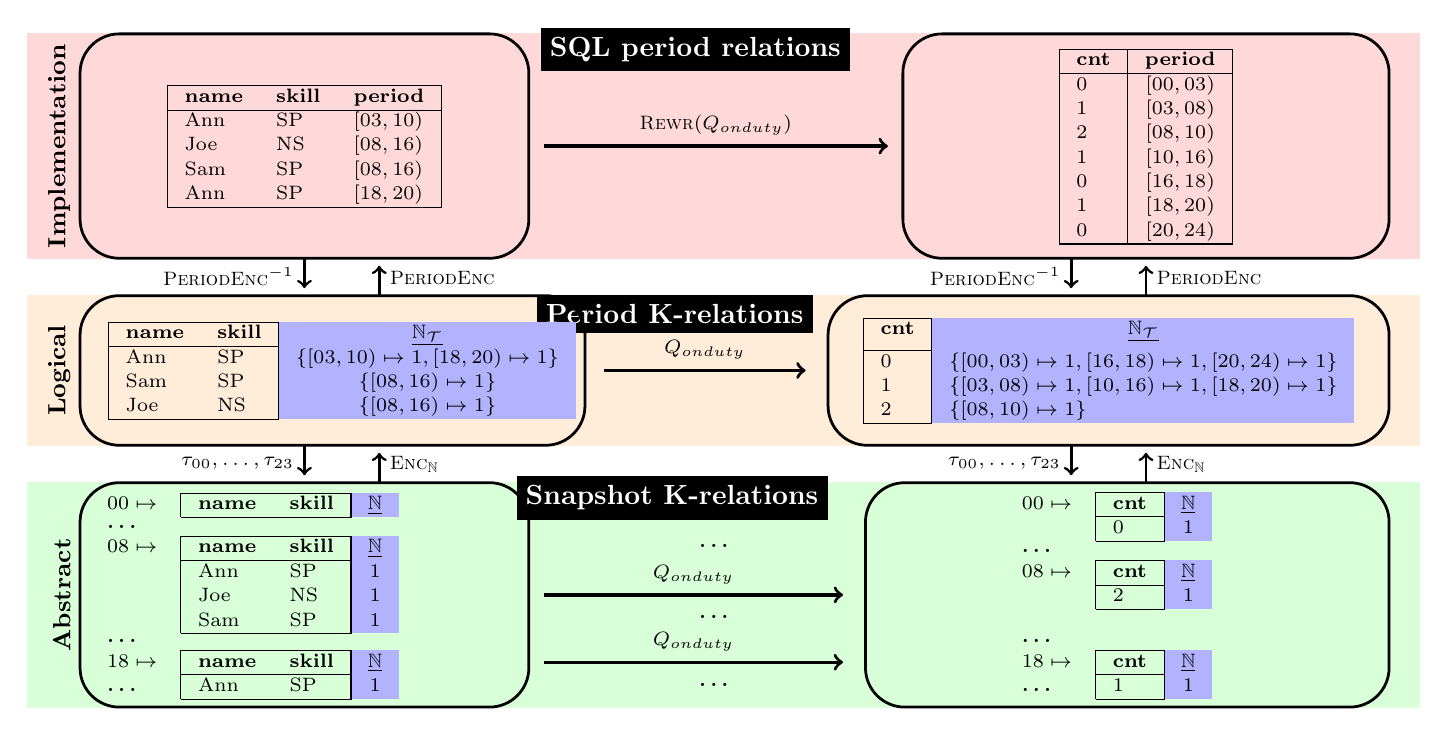
\begin{tikzpicture}[scale=0.95]


\newcommand{\ovfigLeftColumnWidth}{0.4\linewidth}
\newcommand{\ovfigMiddleColumnWidth}{0.09\linewidth}
\newcommand{\ovfigRightColumnWidth}{0.43\linewidth}



  \tikzstyle{every node}=[font=\scriptsize]
  {\renewcommand{\arraystretch}{1.1}

%%%%%%%%%%%%%%%%%%%%%%%%%%%%%%

 % \draw[rounded corners=0.1cm] (-0.7,3.2) rectangle (17.9,-6.2);

  \draw[fill=red!15,line width=0pt,color=red!15] (-0.7,3) rectangle (17.9,-0);
  \draw[fill=orange!15,line width=0pt,color=orange!15] (-0.7,-0.5) rectangle (17.9,-2.5);
  \draw[fill=green!15,line width=0pt,color=green!15] (-0.7,-3) rectangle (17.9,-6);

  \begin{scope}[shift={(0,0)}]

    \node[above, rotate=90] at (0,1.5) {{\bf \small Implementation}};
    \node[color=white, fill=black, above left] at (10.3,2.5) {{\normalsize \bf \SQLrels{}}};

    \draw [rounded corners=0.5cm, line width=1pt] (0,0) rectangle ++(6,3);
    \node at (3,1.5) {
      \begin{tabular}{|lll|}
			%\multicolumn{3}{l}{\textbf{works}} \\
			\cline{1-3}
			\thead{name} &\thead{skill} & \thead{period}\\
			\cline{1-3}
			Ann & SP & $[03, 10)$ \\
      Joe & NS & $[08, 16)$ \\
			Sam & SP & $[08, 16)$ \\
      Ann & SP & $[18, 20)$ \\
			\cline{1-3}
		  \end{tabular}
    };
    \draw[rounded corners=0.5cm, line width=1pt] (11,0) rectangle ++(6.5,3);
    \node at (14.25,1.5) {
  		\begin{tabular}{|l|c|}
  			\cline{1-2}
  			\thead{cnt} & \thead{period}\\
  			\cline{1-2}
  			0 & $[00, 03)$ \\
  			1 & $[03, 08)$ \\
  			2 & $[08, 10)$ \\
  			1 & $[10, 16)$ \\
  			0 & $[16, 18)$ \\
        1 & $[18, 20)$ \\
        0 & $[20, 24)$ \\
  			\cline{1-2}
  		\end{tabular}
    };
    \draw[->, very thick] (6.2,1.5) -- ++(4.6,0) node[pos=0.5, above] {$\reprRewr(Q_{onduty})$};
  \end{scope}


  \draw[->, line width=1pt] (3, 0) -- (3, -0.4) node[pos=0.6, left] {$\reprN^{-1}$};
  \draw[->, line width=1pt] (4, -0.5) -- (4, -0.1) node[pos=0.6, right] {$\reprN$};

  \draw[->, line width=1pt] (13.25, 0) -- (13.25, -0.4) node[pos=0.6, left] {$\reprN^{-1}$};
  \draw[->, line width=1pt] (14.25, -0.5) -- (14.25, -0.1) node[pos=0.6, right] {$\reprN$};

%%%%%%%%%%%%%%%%%%%%%%%%%%%%%%
  \begin{scope}[shift={(0,-3)}]

    \node[above, rotate=90] at (0,1.5) {{\bf \small Logical}};
    \node[color=white, fill=black, above left] at (9.8,2) {{\normalsize \bf Period K-relations}};

    \draw [rounded corners=0.5cm, line width=1pt] (0,0.5) rectangle ++(6.75,2);
    \node at (3.5,1.5) {
  		\begin{tabular}{|ll|c}
  			\cline{1-2}
  			\thead{name} &\thead{skill} & \annotheadcell{$\semTimeNIN$}\\
  			\cline{1-2}
  			Ann & SP & \annotcell{$\{[03, 10) \mapsto 1, [18,20) \mapsto 1\}$} \\
  			Sam & SP & \annotcell{$\{[08, 16) \mapsto 1 \}$} \\
  			Joe & NS & \annotcell{$\{[08, 16) \mapsto 1\}$} \\
  			\cline{1-2}
  		\end{tabular}
    };
    \draw[rounded corners=0.5cm, line width=1pt] (10,0.5) rectangle ++(7.5,2);
    \node at (13.75,1.5) {
  		\begin{tabular}{|l|l}
  			\cline{1-1}
  			\thead{cnt} & \multicolumn{1}{c}{\annotheadcell{$\semTimeNIN$}}\\[1mm]
  			\cline{1-1}
            0 & \annotcell{$\{ [00, 03) \mapsto 1, [16, 18) \mapsto 1,[20, 24) \mapsto 1 \}$} \\
            1 & \annotcell{$\{ [03, 08) \mapsto 1, [10, 16) \mapsto 1 ,[18, 20) \mapsto 1\}$} \\
  			    2 & \annotcell{$\{ [08, 10) \mapsto 1\}$} \\

            \cline{1-1}
  			\cline{1-1}
  		\end{tabular}
    };
    \draw[->, very thick] (7,1.5) -- ++(2.7,0) node[pos=0.5, above] {$Q_{onduty}$} ;
  \end{scope}

  \draw[->, line width=1pt] (3, -2.5) -- (3, -2.9) node[pos=0.6, left] {$\tSlice{00}, \ldots, \tSlice{23}$};
  \draw[->, line width=1pt] (4, -3) -- (4, -2.6) node[pos=0.6, right] {$\repr_{\semN}$};

  \draw[->, line width=1pt] (13.25, -2.5) -- (13.25, -2.9) node[pos=0.6, left] {$\tSlice{00}, \ldots, \tSlice{23}$};
  \draw[->, line width=1pt] (14.25, -3) -- (14.25, -2.6) node[pos=0.6, right] {$\repr_{\semN}$};

  %%%%%%%%%%%%%%%%%%%%%%%%%%%%%%
    \begin{scope}[shift={(0,-6)}]

      \node[above, rotate=90] at (0,1.5) {{\bf \small \revc{Abstract}}};
      \node[color=white,fill=black, above left] at (10,2.5) {{\normalsize \bf Snapshot K-relations}};

      \draw [ rounded corners=0.5cm, line width=1pt] (0,0) rectangle ++(6,3);
      \node at (2.2,2.7) {
        \begin{tabular}{l|ll|c}
          \cline{2-3}
           $00 \mapsto {}$ & \thead{name} &\thead{skill} &  \annotheadcell{$\semN$}\\
          \cline{2-3}
        \end{tabular}
      };
      \node at (2.2,1.8) {
        \begin{tabular}[t]{l|ll|c}
          \multicolumn{2}{l}{{\bf \ldots}} & \multicolumn{1}{l}{} &\\
          \cline{2-3}
           $08 \mapsto {}$ & \thead{name} &\thead{skill} &  \annotheadcell{$\semN$}\\
           \cline{2-3}
           & Ann & SP & \annotcell{1} \\
           & Joe & NS & \annotcell{1} \\
           & Sam & SP & \annotcell{1} \\
          \cline{2-3}
        \end{tabular}
      };
      \node at (2.2,0.6) {
        \begin{tabular}[t]{l|ll|c}
          \multicolumn{2}{l}{{\bf \ldots}} & \multicolumn{1}{l}{} &\\
          \cline{2-3}
           $18 \mapsto {}$ & \thead{name} &\thead{skill} &  \annotheadcell{$\semN$}\\
           \cline{2-3}
           \multicolumn{1}{l|}{{\bf \ldots}} & Ann & SP & \annotcell{1} \\
          \cline{2-3}
        \end{tabular}
      };

      \draw[rounded corners=0.5cm, line width=1pt] (10.5,0) rectangle ++(7,3);
      \node at (13.75,2.55) {
        \begin{tabular}{l|l|c}
          \cline{2-2}
           $00 \mapsto {}$ & \thead{cnt} &  \annotheadcell{$\semN$}\\
           \cline{2-2}
            & 0 & \annotcell{1} \\
          \cline{2-2}
        \end{tabular}
      };
      \node at (13.75,1.8) {
        \begin{tabular}{l|l|c}
          \multicolumn{2}{l}{{\bf \ldots}} & \multicolumn{1}{l}{}\\
          \cline{2-2}
           $08 \mapsto {}$ & \thead{cnt} &  \annotheadcell{$\semN$}\\
           \cline{2-2}
            & 2 & \annotcell{1} \\
          \cline{2-2}
        \end{tabular}
      };
      \node at (13.75,0.6) {
        \begin{tabular}{l|l|c}
          \multicolumn{2}{l}{{\bf \ldots}} & \multicolumn{1}{l}{}\\
          \cline{2-2}
           $18 \mapsto {}$ & \thead{cnt} &  \annotheadcell{$\semN$}\\
           \cline{2-2}
            {\bf \ldots}& 1 & \annotcell{1} \\
          \cline{2-2}
        \end{tabular}
      };
      % \draw[->, very thick] (7.2,2.5) -- ++(2.6,0) node[pos=0.5, above] {$Q_{onduty}
      % %(\tSlice{00}(\textbf{works}))
      % $} ;
      \node at (8.5, 2.15) {{\bf \ldots}};
      \draw[->, very thick] (6.2,1.5) -- ++(4,0) node[pos=0.5, above] {$Q_{onduty}
      %(\tSlice{08}(\textbf{works}))
      $} ;
      \node at (8.5, 1.2) {{\bf \ldots}};
      \draw[->, very thick] (6.2,0.6) -- ++(4,0) node[pos=0.5, above] {$Q_{onduty}
      %(\tSlice{18}(\textbf{works}))
      $} ;
      \node at (8.5, 0.3) {{\bf \ldots}};
    \end{scope}

  }

  \end{tikzpicture}
  \caption{Overview of our approach. Our \emph{\revc{abstract} model} is
  \emph{snapshot K-relations} and nontemporal queries over snapshots (snapshot semantics). Our
  \emph{logical} model is \emph{period K-relations} and % temporal
  queries
  corresponding to the \reva{abstract} model's snapshot queries. % in the \revc{abstract} model.
  Our
  \emph{implementation} uses \emph{\SQLrels{}} and
  rewritten non-temporal queries implementing the other model's snapshot queries. % of the two other models.
  Each model is associated with
  transformations to the other models % below and above
  which commute with queries (modulo the rewriting $\reprRewr$ when mapping to the implementation). % As we will demonstrate, all of these transformations commute with queries (modulo the rewriting $\reprRewr$ when translating from the logical model to the implementation).
} % e.g., for any period K-database $D$, query $Q$, and timepoint $\tPoint$ we have $\query(\tSlice{\tPoint}(D)) = \tSlice{\tPoint}(\query(D))$, which is \emph{snapshot-reducibility}.}
  \label{fig:overview-approach}
\end{figure*}

%%% Local Variables:
%%% mode: latex
%%% TeX-master: "../pvldb.tex"
%%% End:


%%%%%%%%%%%%%%%%%%%%%%%%%%%%%%%%%%%%%%%%
\parttitle{\revc{Abstract} model -- Snapshot $\semK$-relations}
\label{sec:conc-level-seuq}
%
As an \emph{\revc{abstract} model} we use snapshot relations which map time
points to snapshots. Queries over such relations are evaluated over
each snapshot, which trivially satisfies snapshot-reducibility.  To
support both sets and multisets, we introduce
\emph{snapshot $\semK$-relations}~\cite{GK07}, which are
snapshot relations where each snapshot is a $\semK$-relation.  In a
$\semK$-relation, each tuple is annotated with an element from a
domain $\semK$. % that forms a commutative semiring.
For example,
relations annotated with elements from the semiring $\semN$ (natural
numbers) correspond to multiset semantics. % and relations annotated with
% elements from the boolean semiring $\semB$ to set semantics.
%
The result of a snapshot query $\query$ over a snapshot
$\semK$-relation is the result of evaluating $\query$ over the
$\semK$-relation at each time point.

\begin{exam}[\revc{Abstract} Model]
  Figure~\ref{fig:overview-approach} (bottom) shows the snapshots at
  times \texttt{00}, \texttt{08}, and \texttt{18} of an encoding of
  the running example as snapshot $\semN$-relations.  Each snapshot
  is an $\semN$-relation where tuples are annotated with their
  multiplicity (shown % on the right of each tuple
  with shaded
  background). For instance, the snapshot at time \texttt{08} has
  three tuples, each with multiplicity 1. The result of query
  $\qAggEx$ is shown on the bottom right.  Every snapshot in the
  result is computed by running $\qAggEx$ over the corresponding
  snapshot in the input.  For instance, at time \texttt{08} there are
  two SP workers, i.e., $cnt = 2$.
\end{exam}

\parttitle{Logical Model -- Period $\semK$-relations}
\label{sec:logical-level}
%
  % \revdel{
  %   We introduce \periodKrels{} as a \emph{logical model}.
  %   \CapPeriodKrels{} are a compact encoding of temporal data that generalizes
  %   period relations. In a \emph{\periodKrel{}}, every tuple is annotated with a
  %   \textit{temporal $\semK$-element} which is a unique interval-based
  %   representation of the tuple's complete history. This avoids splitting a
  %   tuple's history across multiple tuples.
  % }
%
\revm{We introduce \periodKrels{} as a \emph{logical model}, which merges
equivalent tuples over all snapshots from the abstract model into one tuple. In
a \emph{\periodKrel{}}, every tuple is annotated with a \textit{temporal
$\semK$-element} that is a unique interval-based representation for all time points of the merged tuples from the abstract model.}
%
We define a class of semirings called \textit{period semirings} whose elements are temporal $\semK$-elements.
Specifically, for any semiring $\semK$ we can construct a period semiring $\semTimeNI$ whose annotations are temporal $\semK$-elements.
For instance, $\semTimeNIN$ is the period semiring corresponding to semiring $\semN$ (multisets).
% \revdel{Furthermore, we present a bijective transformation $\repr_{\semK}$ that constructs a \periodKrel{} from a sequenced $\semK$-relation.}
We define necessary conditions for an interval-based model to
correctly encode \SKrels{}  and prove that
\periodKrels{} fullfil these conditions.  Specifically, we call an
interval-based model a \emph{representation system} iff
 the encoding of every \SKrel{} $R$ is (i) unique and (ii) snapshot-equivalent to $R$.
% (i) the encoding for any relation $R$ is unique.
% (ii)
Furthermore, (iii) queries over encodings are
snapshot-reducible. % , and
% (iii).

\begin{exam}[Logical Model]
  Figure~\ref{fig:overview-approach} (middle) shows an encoding of the
  running example as \periodKrels{}.
  % \revdel{
  %   Each tuple is annotated with its complete history, represented as pairs
  %   which consist of a time interval and the tuple's multiplicity (an
  %   annotation from semiring $\semN$) during this time interval. These
  %   annotations are elements of the period semiring $\semTimeNIN$. For
  %   instance, the result tuple with $cnt = 0$ has multiplicity $1$ during the
  %   time intervals $[00, 03)$, $[16,18)$, and $[20,24)$.
  % }
  \revm{For instance, all tuples $(Ann,SP)$ from the abstract model are merged
  into one tuple in the logical model with annotation $\{[03, 10) \mapsto 1,
  [18,20) \mapsto 1\}$, because at each time point during $[03, 10)$ and
  $[18,20)$ a tuple $(Ann,SP)$ with multiplicity $1$ exists.}
%
  In Section~\ref{sec:snapshot-k-relations-1}, we will introduce a mapping
  $\repr_{\semN}$ from snapshot $\semN$ to $\semTimeNIN$-relations and the  \textit{time slice} operator $\tSlice{\tPoint}$ which restores
the snapshot at time $\tPoint$.

\end{exam}

\parttitle{Implementation -- SQL Period Relations}
\label{sec:impl-level}
%
To ensure compatibility with the SQL % :2011
standard, we use % standard period relations (also denoted as
\emph{\SQLrels{}} in our \emph{implementation} and translate snapshot
semantics queries into SQL queries over these period relations.
% To be compatible with SQL:2011's period relations, we define an
% encoding of $\semTimeNIN$-relations as period multiset relations and
% demonstrate how queries with sequenced semantics can be translated
% into equivalent standard SQL queries with multiset semantics over this
% encoding using a rewriting $\reprRewr$.
For this we define an encoding of $\semTimeNIN$-relations as \SQLrels{} ($\reprN$) together with a rewriting scheme for
queries ($\reprRewr$).

\begin{exam}[Implementation]
  Consider the \SQLrels{} shown on the top of
  Figure~\ref{fig:overview-approach}.  Each interval-annotation pair
  of a temporal $\semN$-element in the logical model is encoded as a
  separate tuple in the implementation.
  % \revdel{
  %   For instance, the tuple $(\mathit{Ann},\mathit{SP})$ in the logical
  %   model is encoded as two tuples, each of which records one of the two
  %   intervals during which the tuple exists.
  % }
  \revm{For instance, the annotation of tuple $(Ann,SP)$ from the logical model
  is encoded as two tuples, each of which records one of the two intervals from
  this annotation}
\end{exam}

We present an implementation of our framework as a database middleware
that exposes snapshot semantics as a new language feature in
SQL and rewrites snapshot queries into SQL queries over
\SQLrels{}.  That is, we directly evaluate
snapshot queries over data stored natively as period relations.
%
% \revdel{Since many temporal query languages support snapshot semantics, our
% results enable the efficient and correct implementation of snapshot
% queries specified in these languages.}


\newpage
%%%%%%%%%%%%%%%%%%%%%%%%%%%%%%%%%%%%%%%%%%%%%%%%%%%%%%%%%%%%%%%%%%%%%%%%%%%%%%%%
\section{Snapshot K-relations} % and Snapshot Semantics} % (Abstract Temporal K-relations)}
\label{sec:snapshot-k-relations}

We first review background on the semiring annotation framework ($\semK$-relations). Afterwards,  we define  \textit{snapshot $\semK$-relations} as our \revc{abstract}
model and snapshot semantics for this model. Importantly, queries over snapshot $\semK$-relations are snapshot-reducible by construction. Finally, we state requirements for a logical model to be a representation system
for this \revc{abstract} model.

%%%%%%%%%%%%%%%%%%%%%%%%%%%%%%%%%%%%%%%%%%%%%%%%%%%%%%%%%%%%%%%%%%%%%%%%%%%%%%%%
\subsection{K-relations}
\label{sec:k-relations}

%We now introduce the semiring annotation framework~\cite{GK07} underlying $\semK$-relations. % , the type of annotated relations we will use for interval-based encoding of temporal annotated databases.
In a $\semK$-relation~\cite{GK07}, every tuple is annotated with an
element from a domain $K$ of a commutative semiring $\semK$. % of annotations.
% \revdel{By selecting an appropriate domain $K$, this framework can be tailored for a wide variety of purposes.}
% \revdel{
% For instance, to
% model multiset semantics we annotate each tuple with its multiplicity
% (i.e., an element from the natural numbers $\semN$). $\semK$-relations
% also support many extensions of the relational model including
% incomplete databases, trust, and provenance. %various provenance models (e.g., Lineage).
% }
%
%The semiring framework requires the domain $K$ to be a commutative semiring.
A structure $(\semK, \addK, \multK, \zeroK, \oneK)$ over a set $K$
with binary operations $\addK$ and $\multK$
% where addition $+_\semK: K \times K \to K$ and multiplication
% $\cdot_\semK: K \times K \to K$ are binary operations  over $K$
is a commutative semiring iff (i) addition and
multiplication are commutative, associative, and have a neutral element ($\zeroK$ and $\oneK$, respectively);
(ii) multiplication distributes over addition; and (iii) multiplication with zero
returns zero. Abusing notation, we
will   use $\semK$ to denote both a semiring structure as well as its
  domain.

% That is,
% $K$ is equipped with
% two binary operations $+_\semK: K \times K \to K$ and
% $\cdot_\semK: K \times K \to K$ with neutral elements
% $0_\semK \in K$ and $1_\semK \in K$, respectively.

% and (b) the resulting structure
% is a commutative semiring $\semK = (K,+_{\semK},$
% $\cdot_{\semK},0_{\semK},1_{\semK})$.
% \footnote{Abusing notation, we
%   use $\semK$ to denote both a semiring structure as well as its
%   domain.}
%

% \revdel{The semiring addition and multiplication operations  are used to define how
% annotations propagate through queries.}
% \revdel{The fact that $\semK$ is a commutative semiring guarantees that expected algebraic equivalences
% hold over $\semK$-relations.}
Consider a universal countable domain $\uDom$
of values. % Formally,
An n-ary $\semK$-relation $R$ over $\uDom$ is a
(total) function that maps tuples
 (elements from $\uDom^n$)
to elements from $\semK$ with the convention that tuples mapped to
$0_\semK$ are not in the
relation. Furthermore, we require that $R(t) \neq 0_{\semK}$ only
holds for finitely many $t$.  Two semirings are of particular interest
to
us: % $(\mathbb{N}, +, \cdot, 0, 1)$ (natural numbers with standard arithmetics) encodes multiset semantics while
    % $(\mathbb{B}, \vee, \wedge, false, true)$ (boolean values \textit{true} and \textit{false} with $\vee$ as addition and $\wedge$ as multiplication) corresponds to set semantics.
% The table below shows two
% semirings that are of special interest to us since they encode set and multiset
% semantics.
% %
% \begin{center}
% {\small
%   \begin{tabular}{|cc|}
%     \thead{Semiring} & \thead{Corresponding Model} \\
%     $(\mathbb{B}, \vee, \wedge, 0, 1)$ & Set semantics\\
%     $(\mathbb{N}, +, \cdot, 0, 1)$ & Multiset semantics\\
%     % $({\cal P}(X) \union \{\linNoProv\}, \union_+, \union_\cdot, \linNoProv, \emptyset)$ & Lineage\\
%     % $(\semNX, +, \cdot, 0, 1)$ & Provenance polynomials\\
%     \hline
%   \end{tabular}\\[1mm]
% }
% \end{center}
%
The semiring $(\mathbb{B}, \vee, \wedge, false, true)$ with elements \textit{true} and \textit{false} using
$\vee$ as addition and $\wedge$ as multiplication corresponds to set semantics.
The semiring $(\mathbb{N}, +, \cdot, 0, 1)$ of natural numbers with standard arithmetics
corresponds to multisets. % semantics.

%%%%%%%%%%%%%%%%%%%%%%%%%%%%%%%%%%%%%%%%
% \subsubsection{Queries over K-relations}
% \label{sec:queries-over-k}

The operators of the positive relational algebra\revc{~\cite{DBLP:reference/db/Sirangelo09c}} ($\raPlus$) over
$\semK$-relations are defined by applying the $+_\semK$ and
$\cdot_\semK$ operations of the semiring $\semK$ to input
annotations. Intuitively, the $+_\semK$ and $\cdot_\semK$ operations
of the semiring correspond to the alternative and
conjunctive use of tuples, respectively. For instance, if an output tuple $t$ is
produced by joining two input tuples annotated with $k$ and $k'$, then
the tuple $t$ is annotated with $k \cdot_\semK k'$. Below we provide
the standard definition of $\raPlus$ over
$\semK$-relations~\cite{GK07}. For a tuple $t$, we use $t.A$ to denote the projection
of $t$ on a list of projection expressions $A$ and $t[R]$ to
denote the projection of $t$ on the attributes of relation
$R$. For a condition $\theta$ and tuple $t$, $\theta(t)$ denotes a
function that returns $1_{\semK}$ if $t \models \theta$ and
$0_{\semK}$ otherwise.

%%%%%%%%%%%%%%%%%%%%%%%%%%%%%%%%%%%%%%%%
\begin{defi}[$\raPlus$ over $\semK$-relations]
  Let $\semK$ be a semiring, $R$, $S$ denote $\semK$-relations,
 $t$, $u$ denote
  tuples of appropriate arity, and $k \in K$.  % The positive relational algebra
  $\raPlus$ on
  $\semK$-relations is defined as:
%
\begin{align*}
  \selection_\theta(R)(t) &= R(t) \cdot \theta(t) && (\text{selection}) \\
  \projection_A(R)(t) &= \sum\nolimits_{u: u.A = t} R(u) && (\text{projection}) \\
  (R \join S)(t) &= R(t[R]) \cdot S(t[S]) && (\text{join}) \\
  (R \union S)(t) &= R(t) + S(t) && (\text{union})
  % \emptyset(t) &= 0_{\semK}  && (\text{empty relation}) \\
% \end{align*}\\[-8mm]
% \begin{align*}
%%%%%%%%%%
%
% \end{align*}\\[-8mm]
% \begin{align*}
%%%%%%%%%%
%%%%%%%%%
 %\tag{for any $\schemaOf{R} \union \schemaOf{S}$ tuple $t$}
\end{align*}
\end{defi}
%%%%%%%%%%%%%%%%%%%%%%%%%%%%%%%%%%%%%%%%

% In the following,
We will make use of homomorphisms, functions from
the domain of a semiring $\semK_1$ to the domain of a semiring
$\semK_2$ % {\color{red} ??} between semirings
that % are well-behaved, i.e.,
commute with the semiring operations.  Since $\raPlus$ over $\semK$-relations is defined in terms
of these operations, it follows that semiring homomorphisms commute
with queries, as was proven in~\cite{GK07}.

%%%%%%%%%%%%%%%%%%%%%%%%%%%%%%%%%%%%%%%%
\begin{defi}[Homomorphism]
A mapping $\homo: \semK_1 \to \semK_2$
% from semiring $\semK_1$ to semiring $\semK_2$
is called a homomorphism iff for all $k,k'\in \semK_1$:
\begin{align*}
\homo(0_{\semK_1}) &= 0_{\semK_2}
&\homo(1_{\semK_1}) &= 1_{\semK_2}\\
\homo(k +_{\semK_1} k') &= \homo(k) +_{\semK_2} \homo(k')
&\homo(k \cdot_{\semK_1} k') &= \homo(k) \cdot_{\semK_2} \homo(k')
\end{align*}
\end{defi}
%%%%%%%%%%%%%%%%%%%%%%%%%%%%%%%%%%%%%%%%

%%%%%%%%%%%%%%%%%%%%%%%%%%%%%%%%%%%%%%%%
\begin{exam}
  Consider the $\semN$-relations shown below which are non-temporal versions of our running example. Query $Q = \projection_{mach}($
  $works \join assign)$ returns machines for which there are workers with the right skill to operate the machine.
  Under multiset semantics we expect M1 to occur in the
  result of $Q$ with multiplicity $8$ since $(M1,SP)$ joins with
  $(Pete, SP)$ and  with
  $(Bob, SP)$. Evaluating the query in $\semN$ yields the expected
  result by multiplying the annotations of these join partners. Given
  the $\semN$ result of the query, we can compute the result of the
  query under set semantics by applying a homomorphism $h$ which maps
  all non-zero annotations to $\textit{true}$ and $0$ to
  $\textit{false}$. For example, for result $(M1)$ we get
  $h(8) = true$, i.e., this tuple is in the result under set
  semantics.

  \medskip
\noindent
  \begin{minipage}{0.3\linewidth}
\centering
{\scriptsize\upshape
    \begin{tabular}{|cc|r}
      \multicolumn{3}{l}{\textbf{$\bf works$}} \\
      \cline{1-2}
       \thead{name} & \thead{skill} & \annotcell{$\semN$}\\
       \cline{1-2}
       Pete & SP & \annotcell{$1$}\\
       Bob & SP & \annotcell{$1$} \\
       Alice & NS & \annotcell{$1$}\\
      \cline{1-2}
    \end{tabular}
}
\end{minipage}
\begin{minipage}{0.3\linewidth}
\centering
{\scriptsize\upshape
    \begin{tabular}{|cc|r}
      \multicolumn{3}{l}{\textbf{$\bf assign$}} \\
      \cline{1-2}
       \thead{mach} & \thead{skill} & \annotcell{$\semN$}\\
       \cline{1-2}
       M1 & SP & \annotcell{$4$}\\
       M2 & NS & \annotcell{$5$} \\
      \cline{1-2}
    \end{tabular}
}
\end{minipage}
\begin{minipage}{0.35\linewidth}
    \centering
    {\scriptsize\upshape
    \begin{tabular}{|c|l}
      \multicolumn{2}{l}{\textbf{Result}} \\
      \cline{1-1}
       \thead{A} & \annotcell{$\semN$}\\
       \cline{1-1}
  M1 &       \annotcell{$1 \cdot 4 + 1 \cdot 4 = 8$}\\
  M2 &       \annotcell{$5 \cdot 1 = 5$} \\
      \cline{1-1}
    \end{tabular}
}
  \end{minipage}
\end{exam}
%%%%%%%%%%%%%%%%%%%%%%%%%%%%%%%%%%%%%%%%

%\BG{NOT USED ANYMORE HERE AND INTRODUCED LATER ANYWAYS: In the following, we will often represent annotated relations as sets of tuples that are paired with their annotations. For instance, $R(t) = k$ is represented as $t : k$. }

%%%%%%%%%%%%%%%%%%%%%%%%%%%%%%%%%%%%%%%%
\subsection{Snapshot K-relations} % and Snapshot Semantics}
\label{sec:snapshot-k-relations-1}

We now formally define snapshot
$\semK$-relations, snapshot semantics over such relations, and then define representation systems.  We assume a totally ordered and finite domain
$\timeDomain$ of time points and use $\tLeq$ to denote its order.
$\tMin$ and $\tMax$ denote the minimal and maximal (exclusive) time
point in $\timeDomain$ according to $\tLeq$, respectively. We use $\tPoint + 1$ to denote the successor of % time point
$\tPoint \in \timeDomain$ according to % the order
$\tLeq$.

% Formally, given a finite, totally ordered domain of time $\timeDomain$,
% A \textit{snapshot relation} $\rel$ is a function from $\timeDomain$ to relation instances.




% \BG{ADD BACK IN CASE WE GET TO THAT: Relaxations of this assumption will be discussed later.}
%A snapshot temporal database records the state of the database valid at each point in time. In contrast to previous work that focuses on modelling set or multiset semantics versions of snapshot temporal databases, we aim to developed a general model for adding time to any K-database. % Thus, for a given time point, the state of the database at this point in time would be a K-database. % Note that by defining snapshot databases in this fashion we also cover set and multiset semantics through the use of semirings $\semB$ and $\semN$, respectively.
% As is customary in temporal databases we distinguish between snapshot temporal databases and interval-based encodings.
% Given a database schema $\dbSchema$, we model an abstract temporal $\semK$-database as a function $\timeDomain \to \kDBDom{\semK}{\dbSchema}$ where $\kDBDom{\semK}{\dbSchema}$ is the set of all $\semK$-instances with schema $\dbSchema$.
A \SKrel{} over a relation schema $\relSchema$ is a function $\timeDomain \to \kRelDom{\semK}{\relSchema}$, where $\kRelDom{\semK}{\relSchema}$ is the set of all $\semK$-relations with schema $\relSchema$. \CapSKdbs{} are defined analog. We use $\kDBDom{\timeDomain,\semK}{}$ to denote the set of all
\SKdbs{} for time domain $\timeDomain$.

%%%%%%%%%%%%%%%%%%%%%%%%%%%%%%%%%%%%%%%%
\begin{defi}[Snapshot $\semK$-relation]\label{def:snapshot-k-rel}
  Let $\semK$ be a commutative semiring and $\relSchema$ a relation
  schema. A \SKrel{} $\rel$ is a function
  $\rel : \timeDomain \to \kRelDom{\semK}{\relSchema}$.
\end{defi}
%%%%%%%%%%%%%%%%%%%%%%%%%%%%%%%%%%%%%%%%

For instance, a snapshot $\semN$-relation is shown in
Figure~\ref{fig:overview-approach} (bottom). Given a \SKrel{}, we use the
\textit{timeslice operator}~\cite{DBLP:reference/db/JensenS09w} to access its
state (snapshot) at a time point $\tPoint$: % For \SKrel{}s, its definition is straightforward:
%
$$\tSlice{\tPoint}(\rel) = \rel(\tPoint)$$


% %%%%%%%%%%%%%%%%%%%%%%%%%%%%%%%%%%%%%%%%
% \begin{defi}[Timeslice operator]
% \label{def:snapshot-timeslice}
% Let $\rel$ be a \SKrel{} and
% $\tPoint \in \timeDomain$. The timeslice operator
% $\tSlice{\tPoint}(\rel)$ is defined as:
% $$\tSlice{\tPoint}(\rel) = \rel(\tPoint)$$
% \end{defi}
% %%%%%%%%%%%%%%%%%%%%%%%%%%%%%%%%%%%%%%%%


The evaluation of a query $\query$ over a snapshot database (set of snapshot relations)
  $\db$ under \emph{snapshot semantics} returns a snapshot
relation $\query(\db)$ that is constructed as follows: for each time
point $\tPoint \in \timeDomain$ we have
$\query(\db)(\tPoint) = \query(\db(\tPoint))$.
%
Thus, snapshot temporal queries over \SKrels{}
behave like queries over $\semK$-relations for each
snapshot, i.e., their semantics is uniquely determined by the semantics of queries over $\semK$-relations.

%%%%%%%%%%%%%%%%%%%%%%%%%%%%%%%%%%%%%%%%
\begin{defi}[Snapshot Semantics] % for Snapshot $\semK$-relations]
  \label{def:snapshot-k-rel-queries}
  Let $\db$ be a snapshot $\semK$-database and $\query$ be a query. %  expressed in some suitable formalism.
  The result $\query(\db)$ of $\query$ over $\db$ is a snapshot $\semK$-relation that is defined point-wise as follows:
  \begin{align*}
    \forall \tPoint \in \timeDomain: \query(\db)(\tPoint) = \query(\tSlice{\tPoint}(\db))
  \end{align*}
\end{defi}
%%%%%%%%%%%%%%%%%%%%%%%%%%%%%%%%%%%%%%%%

For example, consider the snapshot $\semN$-relation shown at the bottom of Figure~\ref{fig:overview-approach} and the evaluation of $Q_{onduty}$ under snapshot semantics as also shown in this figure. Observe how the query result is computed by evaluating $Q_{onduty}$ over each snapshot individually using multiset ($\semN$) query semantics.
Furthermore, since $\tSlice{\tPoint}(\query(\rel)) = \query(\rel)(\tPoint)$, per
the above definition, the timeslice operator commutes with queries:
$\tSlice{\tPoint}(\query(\rel)) = \query(\tSlice{\tPoint}(\rel))$.
This property is \textit{snapshot-reducibility}. \BGDel{and has been
  established as an important correctness criterion for temporal
  queries, in particular, for snapshot semantics.}{said before}
\BGDel{Also note that so far we do not restrict the class of queries
  or the formalism they are expressed in. The above definition is
  well-defined for any query language over $\semK$-relations, e.g.,
  relational algebra.}{not so important}

\BGDel{Furthermore, from Definition~\ref{def:snapshot-k-rel-queries} follows that equivalence of queries for \SKrels{}  is equivalent to equivalence of queries  for non-temporal $\semK$-relations.

%%%%%%%%%%%%%%%%%%%%%%%%%%%%%%%%%%%%%%%%
\begin{lem}\label{lem:repr-system-eq}
  Let $\query$ and $\query'$ be two queries. Furthermore, let $\equiv_{\semK}$ denote query equivalence for $\semK$-relations and  $\equiv_{\timeDomain,\semK}$ for \SKrels{}. Then
  \begin{align*}
    \query \equiv_{\semK} \query' \Leftrightarrow \query \equiv_{\timeDomain,\semK} \query'
  \end{align*}
\end{lem}
%%%%%%%%%%%%%%%%%%%%%%%%%%%%%%%%%%%%%%%%
}{side track}

%%%%%%%%%%%%%%%%%%%%%%%%%%%%%%%%%%%%%%%%%%%%%%%%%%%%%%%%%%%%%%%%%%%%%%%%%%%%%%%%
\subsection{Representation Systems}
\label{sec:repr-syst}

% \revdel{\CapSKrels{} lead to a clean semantics for snapshot
% queries, but are impractical due to a high level of redundancy. We will investigate
% more compact, interval-based representations of temporal information that have
% a snapshot query semantics that is equivalent with snapshot databases.}
% \revdel{
% Compact encodings of temporal databases have been considered in the past.
% For instance, in~\cite{T96} point-based representations which are equivalent to
% our snapshot $\semB$-databases have been called abstract temporal databases,
% while interval-based encodings have been called concrete temporal databases.
% }

To compactly encode \SKrels{},
 we study
representation systems that consist of a set of representations
$\reprDomain$, a function
$\repr: \reprDomain \to \kDBDom{\timeDomain,\semK}{}$ which associates an encoding in $\reprDomain$ with the
snapshot $\semK$-database it represents, and a
timeslice operator $\tSlice{\tPoint}$ which extracts the snapshot at
time $\tPoint$ from an  encoding.
If $\repr$ is injective, then we use $\repr^{-1}(D)$ to denote the unique encoding associated with $D$.
We use $\tSlice{}$ to
denote the timeslice over both snapshot databases and
representations. It will be clear from the input which
% timeslice
operator $\tSlice{}$ refers to.
%
For such a representation system, % we use the timeslice operator
% $\tSlice{\tPoint}$ to reason about whether two encodings from  $\reprDomain$
% represent the same snapshot database.
we consider two encodings $\db_1$ and
$\db_2$ from $\reprDomain$ to be
\textit{snapshot-equivalent}~\cite{DBLP:reference/db/JensenS09j}
(written as $\db_1 \intervalEq \db_2$)
if they encode the same snapshot $\semK$-database. Note that this is the case if they encode the same snapshots, i.e.,
iff for all
$\tPoint \in \timeDomain$ we have
$\tSlice{\tPoint}(\db_1) = \tSlice{\tPoint}(\db_2)$. For a representation
system to behave correctly, the following conditions have to be met:
1) \textbf{uniqueness}:
for each snapshot $\semK$-database $\db$ there exists a unique element
from $\reprDomain$ representing $\db$;
2)
\textbf{snapshot-reducibility}: the timeslice operator commutes with
queries; and
3) \textbf{snapshot-preservation}: the encoding function $\repr$
preserves the snapshots of the input.

\BGDel{Snapshot $\semK$-relations are easy to understand and provide a clean temporal extension and snapshot temporal query semantics for annotated relations (and, thus, multiset semantics). However, such relations are quite redundant representations since tuples that occur at multiple time points are replicated across multiple instances. Thus, our goal is to study more compact representations of \SKrels{} which have a  query semantics
that is compatible with the snapshot query semantics over \SKrels{}.}{redundant}



\BGDel{For such a representation system to behave ``correctly'', we have to require that the timeslice operator yields the same result as the timeslice over snapshot relations and that query semantics are snapshot-reducible, i.e., they correctly implement snapshot semantics.}{Explained above now}

%%%%%%%%%%%%%%%%%%%%%%%%%%%%%%%%%%%%%%%%
\begin{defi}[Representation System]\label{def:repr-system}
We call a triple $(\reprDomain, \repr, \tSlice{})$ a \emph{representation system} for % snapshot semantics over
snapshot $\semK$-databases with regard to a class of queries $\qClass$ iff for every snapshot database $\db$, encodings $E$, $E' \in \reprDomain$, time point $\tPoint$, and query $\query \in \qClass$ we have
\begin{enumerate}
\item $\repr(E) = \repr(E') \Rightarrow E=E'$\hfill(uniqness)
  % \db \intervalEq \db' \Rightarrow \repr(\db) = \repr(\db')$ \hfill(uniqness)
\item $% (D,E) \in \repr \Rightarrow
  \tSlice{\tPoint}(\query(E)) = \query(\tSlice{\tPoint}(E))$
\hfill (snapshot-reducibility)
\item $\repr(E) = D \Rightarrow \tSlice{\tPoint}(E) = \tSlice{\tPoint}(\db)$ \hfill (snapshot-preservation)
  %$\query(\repr(\db)) = \repr(\query(\db))$ \hfill \textbf{(Snapshot-reducibility)}
\end{enumerate}
% \begin{enumerate}
% \item $\db \intervalEq \db' \Rightarrow \repr(\db) = \repr(\db')$ \hfill(uniqness)
% \item $\tSlice{\tPoint}(\repr(\db)) = \tSlice{\tPoint}(\db)$ \hfill (snapshot-preservation)
% \item $\tSlice{\tPoint}(\query(\repr(\db)) = \query(\tSlice{\tPoint}(\repr(\db)))$
% \hfill (snapshot-reducibility)
%   %$\query(\repr(\db)) = \repr(\query(\db))$ \hfill \textbf{(Snapshot-reducibility)}
% \end{enumerate}
\end{defi}
%%%%%%%%%%%%%%%%%%%%%%%%%%%%%%%%%%%%%%%%

\BGDel{To see why snapshot-reducibility implies that the implementation of snapshot queries over such encodings is correct, consider the following lemma which proves that to check whether queries under the encoding are equivalent to snapshot semantics queries over \SKrels{} it suffices to prove snapshot-reducibility.}{too much info}
% The following lemma shows that condition $(3)$ we can alternatively check whether the  queries commute with the $\repr$ operator:



% The result of a query $\query$ over an encoding $\db_e = \repr(\db)$ of a snapshost database $\db$ should be snapshot-equivalent to the result of evaluating the query under snapshot semantics over $\db$, i.e., $\query(\db_e) \intervalEq \query(\db)$. Given the definition of snapshot-equivalence that is the case iff $\forall \tPoint \in \timeDomain: \tSlice{\tPoint}(\query(\db_e)) = \query(\tSlice{\tPoint}(\db_e))$, i.e., we have snapshot-reducibility.


%Note that other than the three requirements above we do not prescribe how queries over encodings have to be defined.


\BGDel{
%%%%%%%%%%%%%%%%%%%%%%%%%%%%%%%%%%%%%%%%
\begin{lem}\label{lem:q-commute-eq-snapshot-red}
Consider the 3 conditions of Definitions~\ref{def:repr-system} and condition (4) shown below. We have,
  \begin{align*}
  (1), (2), (4) \Leftrightarrow (1), (2), (3)
  \end{align*}
\begin{align*}
\tSlice{\tPoint}(\query(\repr(\db)) = \query(\tSlice{\tPoint}(\repr(\db)))  \tag{4}
\end{align*}
\end{lem}
%%%%%%%%%%%%%%%%%%%%%%%%%%%%%%%%%%%%%%%%
}{not needed anymore}

\BGDel{When proving our interval-based semiring encodings to be representation systems, we will make use of this lemma.}{No longer needed}

% These requirements together with the defintion of evaluation of implicit queries over temporal databases given above imply that the time slice operator has to commute with queries:

% \begin{align*}
%   \tSlice{\tPoint}(\query(\repr(\db))) &= \tSlice{\tPoint}(\repr(\query(\db)))\\
%                                             &= \query(\db)(\tPoint) = \query(\db(\tPoint))\\
% &= \query(\tSlice{\tPoint}(\repr(\db)))
% \end{align*}



% \begin{defi}[K-timeslice operator]
%   Let K be a semiring, $R$ be a K-relation and $u$ and $v$ be tuples. The
%   K-timeslice operator is defined as follows:

%   \begin{align*}
%     \tau_{t}(R)(u) = \sum_{t \in v.T \land u=v.A} R(v)
%   \end{align*}
% \end{defi}
% \AD{Boris help! I am not used to this ``semiring''-like writing. How do I specify output schema, that the sum belongs to semiring K, and how can I do $t \in v.T$ on the annotation without a concrete data model? Do we need to better define that?}

% \begin{defi}[K-left-exposed]
%   Let K be a semiring, $R$ be a K-relation and $u$ be a tuple. $u$ is K-left-exposed at $t$ in $R$ iff:

%   \begin{align*}
%     \tau_{t}(R)(u) \neq \tau_{t-1}(R)(u)
%   \end{align*}
% \end{defi}

% \begin{defi}[K-right-exposed]
%   Let K be a semiring, $R$ be a K-relation and $u$ be a tuple. $u$ is K-right-exposed at $t$ in $R$ iff:

%   \begin{align*}
%     \tau_{t}(R)(u) \neq \tau_{t+1}(R)(u)
%   \end{align*}
% \end{defi}

% \AD{Ok I think coalescing cannot be defined in an abstract way, since it is a peculiarity of some concrete data models. Am I right?}

% %%%%%%%%%%%%%%%%%%%%%%%%%%%%%%%%%%%%%%%%%%%%%%%%%%%%%%%%%%%%%%%%%%%%%%%%%%%%%%%%
% \subsection{Implicit Temporal Queries over Snapshot K-relations}
% \label{sec:impl-temp-quer}

% \BG{Define semantics of queries over snapshot K-relations based on snapshot-reducibility, i.e., queries have a point-wise semantics, i.e., queries commute with time slice}

%%%%%%%%%%%%%%%%%%%%%%%%%%%%%%%%%%%%%%%%%%%%%%%%%%%%%%%%%%%%%%%%%%%%%%%%%%%%%%%%
\section{Temporal $\semK$-elements}
\label{sec:temporal-k-normalform}

We now introduce temporal $\semK$-elements that are the annotations we use to
define our logical model (representation system).  % which we will later prove to be a representation system for \SKrels{}.
Temporal
$\semK$-elements record, using an interval-based encoding, how the
$\semK$-annotation of a tuple in a \SKrel{} changes over time. We introduce a
unique normal form for temporal $\semK$-elements based on a generalization of
coalescing~\cite{DBLP:conf/vldb/BohlenSS96}.

\subsection{Defining Temporal $\semK$-elements}
\label{sec:concrete-temporal-k}


% %%%%%%%%%%%%%%%%%%%%%%%%%%%%%%%%%%%%%%%%
% \begin{defi}[Abstract Temporal $\semK$-elements]
% Given a semiring $\semK$, an \emph{abstract temporal $\semK$-element} $\anyTE$ is a function $\timeDomain \to \semK$.
% \end{defi}
% %%%%%%%%%%%%%%%%%%%%%%%%%%%%%%%%%%%%%%%%



% %%%%%%%%%%%%%%%%%%%%%%%%%%%%%%%%%%%%%%%%%%%%%%%%%%%%%%%%%%%%%%%%%%%%%%%%%%%%%%%%
% \subsection{Intervals}
% \label{sec:intervals}


To define % a more compact encoding of
temporal $\semK$-elements, we need to introduce some background on
intervals. Given the time domain $\timeDomain$ and its associated
total order $\tLeq$, an interval $\interval = [\tBegin, \tEnd)$ is a
pair of time points from $\timeDomain$, where $\tBegin \tLe \tEnd$.
Interval $\interval$ represents the set of contiguous time points
$\{ \tPoint \mid \tPoint \in \timeDomain \wedge \tBegin \tLeq \tPoint
\tLe \tEnd\}$.
For an interval $\interval = [\tBegin,\tEnd)$ we use
$\iBegin{\interval}$ to denote $\tBegin$ and $\iEnd{\interval}$ to
denote $\tEnd$. We use $I, I', I_1, \ldots $ to represent intervals.
% and $\intervalSet, \intervalSet', \ldots$\BG{Check whether
%   $\intervalSet$ notation is still used anywhere} to denote sets of
% intervals.
We define a relation $\adjacent{\interval_1}{\interval_2}$
that contains all interval pairs that are adjacent:
$\adjacent{\interval_1}{\interval_2} \Leftrightarrow
(\iEnd{\interval_1} = \iBegin{\interval_2}) \vee (\iEnd{\interval_2}
= \iBegin{\interval_1})$.
% where $\iEnd{\interval_1}+1$ denotes the successor of
% $\iEnd{\interval_1}$ in $\timeDomain$ according to $\tLeq$.
%
We will implicitly understand set operations, such as
$t \in \interval$ or $\interval_1 \subseteq \interval_2$, to be
interpreted over the set of points represented by an
interval. Furthermore, $\interval \cap \interval'$ denotes the
interval that covers precisely the intersection of the sets of time
points defined by $\interval$ and $\interval'$ and
$\interval \cup \interval'$ denotes their union (only well-defined if
$\interval \cap \interval' \neq \emptyset$ or
$\adjacent{\interval}{\interval'}$). For convenience, we define
$\interval \cup \interval' = \emptyset$ iff
$\interval \cap \interval' = \emptyset \land \neg
\adjacent{\interval}{\interval'}$.
We use $\intervalDom$ to denote the set of all intervals over
$\timeDomain$.

%%%%%%%%%%%%%%%%%%%%%%%%%%%%%%%%%%%%%%%%
\begin{defi}[Temporal $\semK$-elements]
Given a semiring $\semK$, a \emph{temporal $\semK$-element} $\anyTE$ is a function $\intervalDom \to \semK$. We use $\cTEDom{\semK}$ to denote the set of all such temporal elements for $\semK$.
\end{defi}
%%%%%%%%%%%%%%%%%%%%%%%%%%%%%%%%%%%%%%%%

% In the following we will use the notation for temporal
% $\semK$-elements introduced in Section~\ref{sec:introduction}.
We represent temporal $\semK$-elements  as sets of input-output pairs.  Intervals that are not explicitly mentioned are % assumed to be
mapped
to $0_\semK$. \BGDel{For instance,
  $\{ [\tPoint_1,\tPoint_2] \mapsto k_1, [\tPoint_3,\tPoint_{10}]
  \mapsto k_2 \}$
  is the temporal element that maps all time intervals to $0_\semK$
  except for $[\tPoint_1,\tPoint_2]$ which is mapped to $k_1$ and
  $[\tPoint_3,\tPoint_{10}]$ which is mapped to $k_2$.}{}

%%%%%%%%%%%%%%%%%%%%%%%%%%%%%%%%%%%%%%%%
\begin{exam}\label{ex:temp-k-elem}
Reconsider our running example with $\timeDomain = \{ 00, \ldots, 23
  \}$.
  The history of the annotation of tuple $t = $ \texttt{(Ann,SP)}
  from the \texttt{works} relation is as shown in
  Figure~\ref{fig:overview-approach} (middle). For sake of the example, we change the multiplicity of this tuple to $3$ during $[03,09)$ and $2$ during $[18,20)$. This information is encoded as the temporal
  $\semN$-element $\anyTE_1 = \{[03, 09) \mapsto 3, [18,20) \mapsto 2\}$. % shown below:
  % The abstract temporal $\semN$-element corresponding to the history of  is:
  % Consider the temporal history of tuple $t = $ \textsf{\upshape (Ann,PROD)} as shown in Figure~\ref{fig:example_db}. The abstract temporal $\semN$-element recording how the annotation of $t$ evolved over time is:
 %  \begin{align*}
 % &\anyTE_1 = \{[03, 09) \mapsto 3, [18,20) \mapsto 2\}
 %    %&&\{ \, \tPoint_1 \mapsto 0, &&\tPoint_2 \mapsto 1, &&\tPoint_3 \mapsto 1 \,\}
 %  \end{align*}
  % \begin{align*}
  %   &&1 \mapsto 0 &&2 \mapsto 0 &&3 \mapsto 1 &&\ldots &&6 \mapsto 1 &&7 \mapsto 0 &&\ldots\\ &&10 \mapsto 0 &&11 \mapsto 1 &&12 \mapsto 1 &&13 \mapsto 0 && \ldots &&15 \mapsto 0
  % \end{align*}
\end{exam}
%%%%%%%%%%%%%%%%%%%%%%%%%%%%%%%%%%%%%%%%

Note that a temporal $\semK$-element $\anyTE$ may map overlapping
intervals to non-zero elements of $\semK$.
% \revdel{In principle, we could disallow this, but allowing overlap simplifies the definition of operations over temporal $\semK$-elements.}
We assign the following semantics to overlap: the
annotation at a time point $\tPoint$ recorded by $\anyTE$ is the
sum of the annotations assigned to intervals containing $\tPoint$.
For instance, the annotation at time $04$ for the  $\semN$-element $\anyTE = \{ [00, 05) \mapsto 2, [04, 05) \mapsto 1 \}$ would be $2 + 1 = 3$.
%\jg{This sentence sounds complicated to me}.
To extract the annotation
valid at time $\tPoint$ from a temporal $\semK$-element $\anyTE$, we
define a timeslice operator for temporal $\semK$-elements as follows:
% Let % $\anyTE_1$ be an abstract and
% be $\anyTE$ a temporal $\semK$-element, then
%
\begin{align*}\label{eq:temp-k-elem-timeslice}
% \tSlice{\tPoint}(\anyTE_1) &= \anyTE_1(\tPoint)
  &\tSlice{\tPoint}(\anyTE) = \sum_{% \interval \in \intervalDom \wedge
\tPoint \in \interval} \anyTE(\interval) \tag{timeslice operator}
\end{align*}

% Given two temporal $\semK$-elements, we may want to know whether they represent the same history of annotations.
Given two temporal $\semK$-elements $\anyTE_1$ and $\anyTE_2$, we
would like to know if they represent the same history of annotations.
For that, we define \emph{snapshot-equivalence} ($\intervalEq$) for
temporal $\semK$-elements:
% Let $\anyTE_1$ and $\anyTE_2$ be temporal
% $\semK$-elements.
% written as $\anyTE_1 \intervalEq \anyTE_2$: % based on the d
% efinition of time slice:
\begin{align*}\label{eq:temp-k-element-equivalence}
\anyTE_1 \intervalEq \anyTE_2 \Leftrightarrow \forall \tPoint \in \timeDomain: \tSlice{\tPoint}(\anyTE_1) = \tSlice{\tPoint}(\anyTE_2) \tag{snapshot-equivalence}
\end{align*}

\BGDel{In the temporal database literature, equivalent but representationally different temporal databases have sometimes been called \textit{snapshot-equivalent}. Relation  $\intervalEq$ is  snapshot-equivalence for temporal $\semK$-elements.}{earlier}

% our goal is to study more compact representations of \SKrels{} by using interval encodings of sets of time points and by annotating tuples with their history, and then define a query semantics over these representations that agrees with \SKrel{}al query semantics per Definition~\ref{def:snapshot-k-rel-queries}.



%%%%%%%%%%%%%%%%%%%%%%%%%%%%%%%%%%%%%%%%%%%%%%%%%%%%%%%%%%%%%%%%%%%%%%%%%%%%%%%%
\subsection{A \revc{Normal Form} Based on $\semK$-Coalescing}
\label{sec:coalescing}

The encoding of the annotation history of a tuple as a temporal $\semK$-element is typically not unique.

%%%%%%%%%%%%%%%%%%%%%%%%%%%%%%%%%%%%%%%%
\begin{exam}\label{ex:non-unique-concrete-temp-k-elem}
Reconsider the temporal $\semN$-element $\anyTE_1$ from Example~\ref{ex:temp-k-elem}. Recall that we omit intervals that are mapped to $0$. The $\semN$-elements shown below are snapshot-equivalent to $\anyTE_1$.
  \begin{align*}
    &\anyTE_2 = \{[03, 09) \mapsto 1, [03,06) \mapsto 2, [06,09) \mapsto 2, [18,19) \mapsto 2\} \\[2mm]
    &\anyTE_3 = \{[03, 05) \mapsto 3, [05,09) \mapsto 3, [18,19) \mapsto 2\}
  \end{align*}
\end{exam}
%%%%%%%%%%%%%%%%%%%%%%%%%%%%%%%%%%%%%%%%

To be able to build a representation system based on temporal $\semK$-elements we need a unique way to encode the annotation history of a tuple as a  temporal $\semK$-element (condition 1 of Definition~\ref{def:repr-system}). % (to define $\repr$ as a bijective mapping).
\BGDel{Also from a user perspective there is a benefit in representing a query result in a unique and predictable way.}{Somewhere else?}
That is, we need to define a normal form that is unique for snapshot-equivalent temporal $\semK$-elements. % such that snapshot-equivalent temporal elements are equal if brought into this normal form.
To this end, we generalize \textit{coalescing}, which was defined for temporal databases with set semantics in~\cite{DBLP:journals/tods/Snodgrass87,DBLP:conf/vldb/BohlenSS96}. The generalized form, which we call $\semK$-coalescing, coincides with standard coalescing for semiring $\semB$ (set semantics) and, for any semiring $\semK$, yields a unique encoding. % of snapshot-equivalent temporal $\semK$-elements.

$\semK$-coalescing creates maximal intervals of contiguous time points
with the same annotation. The output is a temporal $\semK$-element such that
(a) no two intervals mapped to a non-zero element overlap and (b)
adjacent intervals assigned to non-zero elements are guaranteed to be
mapped to different annotations. To determine such intervals, we
define annotation changepoints, time points $\tPoint$ where the annotation of a temporal $\semK$-element differs from the annotation at $\tPoint - 1$, i.e., $\tSlice{\tPoint}(\anyTE) \neq \tSlice{\tPoint-1}(\anyTE)$. It will be convenient to also
consider $\tMin$ as an annotation
changepoint. % or which are lower boundary points of $\timeDomain$.

%%%%%%%%%%%%%%%%%%%%%%%%%%%%%%%%%%%%%%%%
\begin{defi}[Annotation Changepoint]\label{def:cp}
  Given a temporal $\semK$-element $\anyTE$, a time point $\tPoint$ is called a \emph{changepoint} in $\anyTE$ if one of the following conditions holds:
  \begin{itemize}
  \item  $\tPoint = \tMin$ % or $\tPoint = \tMax$
    % \wedge \tSlice{\tPoint} > 0$
    \hfill(smallest  time point)
  % \item  $\forall \tPoint' \in \timeDomain: \tPoint' \tLeq \tPoint$  % should not be necessary \wedge \tSlice{\tPoint} > 0$
  %   \hfill(largest time point)
  \item $\tSlice{\tPoint - 1}(\anyTE) \neq \tSlice{\tPoint}(\anyTE)$ \hfill(change of annotation)
  % \item $\tSlice{\tPoint}(\cTE) \neq \tSlice{\tPoint + 1}(\cTE)$ \hfill(right exposed)
  \end{itemize}
  We use $\CPs{\anyTE}$ to denote the set of all annotation
  changepoints for $\anyTE$. Furthermore, we define $\CPIs{\anyTE}$ to
  be the set of all intervals that consist of consecutive change
  points:
  \begin{align*}
    \CPIs{\anyTE} &= \{ [\tPoint_b, \tPoint_e) \mid \tPoint_b \tLe \tPoint_e \wedge \tPoint_b \in \CPs{\anyTE} \wedge{}
    \\
                  &\mathtab\mathtab(\tPoint_e \in \CPs{\anyTE} \vee T_e = \tMax) \wedge{}
    \\
                  &\mathtab\mathtab \not\exists \tPoint' \in \CPs{\anyTE}: \tPoint_b \tLe \tPoint' \tLe \tPoint_e \}
  \end{align*}
\end{defi}
%%%%%%%%%%%%%%%%%%%%%%%%%%%%%%%%%%%%%%%%

In Definition~\ref{def:cp}, $\CPIs{\anyTE}$ computes maximal intervals
such that the annotation assigned by $\anyTE$ to each point in such an
interval is constant. In the coalesced representation of
$\anyTE$ only such intervals are mapped to non-zero annotations. % represented as a single interval.
	% \begin{defi}[covered]
	% 	Given a time point $t$ and a set of intervals $k$, $t$ is covered in $k$ iff $t$ is contained in any interval of $k$, i.e.,
	% 	\begin{align*}
	% 		\exists T \in k : t \in T
	% 	\end{align*}
	% \end{defi}

	% \begin{defi}[left-exposed]
	% 	Given a time point $t$ and a set of intervals $k$, $t$ is left-exposed in $k$ iff the time point before $t$ is not covered by any interval in $k$, i.e.,
	% 	\begin{align*}
	% 		\nexists T \in k : t - 1 \in T
	% 	\end{align*}
	% \end{defi}

	% \begin{defi}[right-exposed]
	% 	Given a time point $t$ and a set of intervals $k$, $t$ is right-exposed in $k$ iff the time point after $t$ is not covered by any interval in $k$, i.e.,
	% 	\begin{align*}
	% 		\nexists T \in k : t + 1 \in T
	% 	\end{align*}
	% \end{defi}

%%%%%%%%%%%%%%%%%%%%%%%%%%%%%%%%%%%%%%%%
\begin{defi}[$\semK$-Coalesce]
 Let $\anyTE$  be a  temporal $\semK$-element.
 We define $\semK$-coalescing $\kCoalesce{\semK}$ as a function $\cTEDom{\semK} \to \cTEDom{\semK}$:
\begin{align*}
\kCoalesce{\semK}(\anyTE)(\interval) & =
                                     \begin{cases}
                                       \tSlice{\iBegin{\interval}}(\anyTE) &\text{if}\; \interval \in \CPIs{\anyTE}\\
                                       \zeroK &\text{otherwise}
                                     \end{cases}
    % & (\forall t \text{ covered by } coalesce(k) \iff t \text{ covered by } k) \land {}\\
    % & (\forall [T_s, T_e] \in coalesce(k) \Rightarrow T_s \text{ is left-exposed in } coalesce(k) \land {} \\
    % & \phantom{(\forall [T_s, T_e] \in coalesce(k) \Rightarrow {}} T_e \text{ is right-exposed in } coalesce(k)
  \end{align*}
  We use $\nTEDom{\semK}$ to denote all normalized temporal $\semK$-elements, i.e., elements $\anyTE$ for which $\kCoalesce{\semK}(\anyTE') = \anyTE$ for some $\anyTE'$. %there exists $\anyTE'$ such that $\anyTE = \kCoalesce{\semK}(\anyTE')$.

\end{defi}
%%%%%%%%%%%%%%%%%%%%%%%%%%%%%%%%%%%%%%%%

%%%%%%%%%%%%%%%%%%%%%%%%%%%%%%%%%%%%%%%%%%%%%%%%%%%%%%%%%%%%%%%%%%%%%%%%%%%%%%%%
\begin{figure}
  \centering
  \scriptsize
  \renewcommand{\arraystretch}{1.2}

  \begin{tabular}[t]{|l|l|}
    \hline
    \thead{sal} & \thead{period} \\
    \hline
    $50$k & $[1,13)$ \\
    $30$k & $[3,13)$ \\
    $30$k & $[3,10)$ \\
    $40$k & $[11,13)$ \\
    \hline
  \end{tabular}
  \hspace{1cm}
  \begin{minipage}[t]{0.35\columnwidth}
    \begin{align*}
      &\anyTE_{50k} = \{[1,13) \mapsto 1 \}\\[1mm]
      &\anyTE_{30k} = \{[3,10) \mapsto 1, [3,13) \mapsto 1 \}\\[1mm]
      &\anyTE_{40k} = \{[11,13) \mapsto 1 \}
    \end{align*}
  \end{minipage}

  \caption{Example period multiset relation $S$ and temporal
    $\semN$-elements encoding the history of tuples.}
  \label{fig:example_temp_coalesce}
\end{figure}
%%%%%%%%%%%%%%%%%%%%%%%%%%%%%%%%%%%%%%%%%%%%%%%%%%%%%%%%%%%%%%%%%%%%%%%%%%%%%%%%


%%%%%%%%%%%%%%%%%%%%%%%%%%%%%%%%%%%%%%%%
\begin{exam}\label{ex:k-coalesce}
  Consider the \SQLrel{} shown in
  Figure~\ref{fig:example_temp_coalesce}. The temporal
  $\semN$-elements encode the history of tuples $(30k)$,
  $(40k)$ and $(50k)$. Note that $\anyTE_{30k}$ is not coalesced since
  the two non-zero intervals of this % temporal
  $\semN$-element
  overlap. Applying $\semN$-coalesce we get:
  %
  \begin{align*}
    \kCoalesce{\semN}(\anyTE_{30k}) = \{ [3,10) \mapsto 2, [10,13) \mapsto 1 \}
  \end{align*}
  %
  That is, this tuple occurs twice within the time interval $[3,10)$
  and once in $[10,13)$, i.e., it has annotation changepoints
  $3$, $10$, and $14$. Interpreting the same relation under set
  semantics (semiring $\semB$), the history of $(30k)$ can be encoded
  as a temporal $\semB$-element
  ${\anyTE_{30k}}' = \{ [3,10) \mapsto true, [3,13) \mapsto true
  \}$. Applying $\semB$-coalesce: % we get:
  \begin{align*}
    \kCoalesce{\semB}({\anyTE_{30k}}') = \{ [3,13) \mapsto true \}
  \end{align*}
  %
  That is, this tuple occurs (is annotated with $true$) within the time interval $[3,13)$ and its annotation changepoints are $3$ and $14$.
\end{exam}
%%%%%%%%%%%%%%%%%%%%%%%%%%%%%%%%%%%%%%%%

We now prove several important properties of the $\semK$-coalesce operator
establishing that $\nTEDom{\semK}$ (coalesced temporal $\semK$-elements) is a good choice for a \revc{normal form} of
 temporal $\semK$-elements.

%%%%%%%%%%%%%%%%%%%%%%%%%%%%%%%%%%%%%%%%
\begin{lem}\label{lem:coalesce-properties}
  Let $\semK$ be a semiring and $\anyTE$, $\anyTE_1$ and $\anyTE_2$  temporal $\semK$-elements. We have:
  \begin{align*}
    \kCoalesce{\semK}(\kCoalesce{\semK}(\anyTE)) &= \kCoalesce{\semK}(\anyTE) \tag{idempotence}\\
    \anyTE_1 \intervalEq \anyTE_2 &\Leftrightarrow \kCoalesce{\semK}(\anyTE_1) = \kCoalesce{\semK}(\anyTE_2) \tag{uniqueness}\\
    \anyTE &\intervalEq \kCoalesce{\semK}(\anyTE) \tag{equivalence preservation}
  \end{align*}
\end{lem}
%%%%%%%%%%%%%%%%%%%%%%%%%%%%%%%%%%%%%%%%
  \proofsketch{We provide the proofs for all lemmas and theorems in a technical report~\cite{DG18}, \revm{but show sketches for important proofs here. Equivalence preservation and uniqueness follow from the fact that annotation change points are defined based on snapshots. Uniqueness plus equivalence preservation implies idempotence.}}
  \iftechreport{
\begin{proof}
  All proofs are shown in Appendix~\ref{sec:proofs}.
\end{proof}
}

%%%%%%%%%%%%%%%%%%%%%%%%%%%%%%%%%%%%%%%%
% 1) the operator is idempotent, i.e., for any temporal element $\anyTE$: $\kCoalesce{\semK}(\kCoalesce{\semK}(\anyTE)) = \kCoalesce{\semK}(\anyTE)$; 2) equivalent temporal elements, i.e., for any temporal elements $\anyTE_1$ and $\anyTE_2$ we have $\anyTE_1 \intervalEq \anyTE_2 \Leftrightarrow \kCoalesce{\semK}(k) = \kCoalesce{\semK}(\anyTE_2)$; and 3)


% Let us recall the definition of coalesce for temporal intervals, that given a set of intervals returns a unique representations of the set of time points covered by the intervals which does not contain any overlapping intervals and no unnecessary splits, e.g., $[1,4)$ instead of $[1,3)$ and $[3,4)$.





% \begin{itemize}
% \item K-coalesce can be redudantly pushed into K-addition
%   $\kCoalesce{\semK}(k +_\semK k') = \kCoalesce{\semK}(\kCoalesce{\semK}(k)
%   +_\semK k')$
% \item K-coalesce can be redudantly pushed into K-multiplication $\kCoalesce{\semK}(k \cdot_\semK k') = \kCoalesce{\semK}(\kCoalesce{\semK}(k) \cdot_\semK k')$
% \end{itemize}


% \BG{difference between abstract (snapshot) and  temporal databases. Introduce snapshot-reducibility (aka implicit temporal semantics) and scope what we are doing (only implicit temporal databases). Representation systems and weakly equivalent, i.e., two different representations for the same}
% \BG{Progression from snapshot K-relations to tuple-annotated databases, this is immediate (annotate tuples with functions from time points to K-elements recording for each time point the corresponding annotation of the tuple).}


%%%%%%%%%%%%%%%%%%%%%%%%%%%%%%%%%%%%%%%%%%%%%%%%%%%%%%%%%%%%%%%%%%%%%%%%%%%%%%%%
\section{Period Semirings}
\label{sec:interv-temp-annot}

Having established a unique normal form of temporal $\semK$-elements,
we now proceed to define period semirings as our logical model. The elements of a period semiring are temporal
$\semK$-elements in normal form. We prove that these structures are
semirings and ultimately that relations annotated with period semirings form a
representation system for snapshot $\semK$-relations for $\raPlus$. In
Section~\ref{sec:complex-queries}, we then prove them to also be a
representation system for $\raAgg$, i.e., queries involving difference
and aggregation.
% ultimately that such annotations are representation
% systems for \SKrels{} for
% a large class of
% queries.

When defining the addition and multiplication operations and their
neutral elements in the semiring structure of temporal
$\semK$-elements, we have to ensure that these definitions are
compatible with semiring $\semK$ on snapshots. Furthermore, we need to
ensure that the output of these operations is guaranteed to be $\semK$-coalesced. The latter can be ensured by applying $\semK$-coalesce to
the output of the operation. For addition, snapshot reducibility
is achieved by pointwise addition (denoted as $\addP$)
of the two functions that constitute the two input temporal
$\semK$-elements. That is, for each interval $\interval$, the function
that is the result of the addition of temporal $\semK$-elements $\anyTE_1$ and
$\anyTE_2$ assigns to $\interval$ the value
$\anyTE_1(\interval) +_{\semK} \anyTE_2(\interval)$. For
multiplication, the multiplication of two $\semK$-elements assigned to
an overlapping pair of intervals $\interval_1$ and $\interval_2$ is
valid during the intersection of $\interval_1$ and
$\interval_2$. Since both input temporal $\semK$-elements may assign non-zero
values to multiple intervals that have the same overlap, the resulting
$\semK$-value at a point $\tPoint$ would be the sum over all pairs of
overlapping intervals. We denote this operation as $\multP$. Since
$\addP$ and $\multP$ may return a temporal $\semK$-element that is not
coalesced, we define the operations of our structures to apply
$\kCoalesce{\semK}$ to the result of $\addP$ and $\multP$.  The zero
element of the temporal extension of $\semK$ is the temporal $\semK$-element
that maps all intervals to $0$ and the $1$ element is the temporal
element that maps every interval to $0_{\semK}$ except for
$[\tMin, \tMax)$ which is mapped to $1_{\semK}$.

%%%%%%%%%%%%%%%%%%%%%%%%%%%%%%%%%%%%%%%%
\begin{defi}[Period Semiring]
  For a time domain $\timeDomain$ with minimum $\tMin$ and maximum
  $\tMax$ and a semiring $\semK$, the period semiring
  $\semTimeNI$ is defined as:
  $$\semTimeNI = (\nTEDom{\semK}, \addNI, \multNI, \zeroNI, \oneNI)$$
  where for $k,k' \in \nTEDom{\semK}$ and :
  \begin{align*}
        \forall \interval \in \intervalDom: \zeroNI(\interval) &= 0_{\semK} &
    % \forall \interval \in \intervalDom:
                                                                              \oneNI(\interval) &=
                             \begin{cases}
                               1_{\semK} &\text{if}\; \interval=[\tMin,\tMax)\\
                               0_{\semK} &\text{otherwise}
                             \end{cases}
  \end{align*}\\[-8mm]
  \begin{align*}
    k \addNI k' &= \kCoalesce{\semK}(k \addP k')\\
\forall \interval \in \intervalDom:
    (k \addP k')(\interval) &= k(\interval) +_{\semK} k'(\interval)\\
    k \multNI k' &= \kCoalesce{\semK}(k \multP k')\\
\forall \interval \in \intervalDom:    (k \multP k')(\interval) &= \sum_{\forall \interval', \interval'': \interval = \interval' \cap \interval''} k(\interval') \cdot_{\semK} k'(\interval'')
  \end{align*}

\end{defi}
%%%%%%%%%%%%%%%%%%%%%%%%%%%%%%%%%%%%%%%%

  %%%%%%%%%%%%%%%%%%%%%%%%%%%%%%%%%%%%%%%%%%%%%%%%%%%%%%%%%%%%%%%%%%%%%%%%%%%%%%%%
%   \begin{figure}
%     \newcommand{\tablewid}{1.6cm}
%       \begin{scriptsize}
% % %%%%%%%%%%%%%%%%%%%%%%%%%%%%%%%%%%%%%%%%
% % \centering{\normalsize \bf Example Query}\\
% % \begin{lstlisting}
% % SELECT sal FROM esal;
% % \end{lstlisting}
%
% % %%%%%%%%%%%%%%%%%%%%%%%%%%%%%%%%%%%%%%%%
% %         \centering{\normalsize \bf Interval-based snapshot query result and possible encoding of tuple annotations as temporal elements}\\
%     {\renewcommand{\arraystretch}{1.2}
%       \begin{tabular}[t]{|ll|l}
%         \multicolumn{3}{l}{\textbf{emp}}\\
%       \cline{1-2}
%               \thead{sal} & \thead{name} & \annotcell{$\nTEDom{\semN}$} \\
%       \cline{1-2}
%          $50$k & Peter & \annotcell{$\{[1,13] \mapsto 1 \}$}\\
%         $30$k & Ann & \annotcell{$\{[3,10] \mapsto 2, [11,13] \mapsto 1\}$} \\
%          $40$k & Ann & \annotcell{$\{[11,13] \mapsto 1\}$} \\
%       \cline{1-2}
%       \end{tabular}} {\renewcommand{\arraystretch}{1.2}
%       \hfill
%     \begin{tabular}[t]{|l|l}
%         \multicolumn{2}{l}{$\mathbf{\projection_{name}(emp)}$}\\
%       \cline{1-1}
%               \thead{sal} & \annotcell{$\nTEDom{\semN}$}\\
%       \cline{1-1}
%          Peter & \annotcell{$\{[1,13] \mapsto 1 \}$}\\
%          Ann & \annotcell{$\{[3,13] \mapsto 2 \}$} \\
%       \cline{1-1}
%     \end{tabular}}
% \end{scriptsize}
%     \caption{Evaluating queries over $\semTimeNIN$-relations.}
%     \label{fig:example-interval-sem-relation}
%   \end{figure}
%%%%%%%%%%%%%%%%%%%%%%%%%%%%%%%%%%%%%%%%%%%%%%%%%%%%%%%%%%%%%%%%%%%%%%%%%%%%%%%%

% %%%%%%%%%%%%%%%%%%%%%%%%%%%%%%%%%%%%%%%%
% \begin{exam}\label{ex:interval-sem-storage-and-query-evaluation}
%   Consider the $\semTimeNIN$-relation \texttt{emp} shown in
%   Figure~\ref{fig:example-interval-sem-relation}. Employee Peter has
%   always earned \$50k. There are two employees named Ann; both earned
%   \$30k until one of them got a raise at time point $11$ and now earns
%   \$40k.  Consider the result of evaluating query
%   $\projection_{name}(emp)$ over this instance as shown in
%   Figure~\ref{fig:example-interval-sem-relation}. Recall the
%   annotation of a tuple $\tuple$ in the result of a projection over a
%   $\semK$-relation is the sum of all input tuples which are projected
%   onto $\tuple$. Let
%   $\anyTE_1 = \{[3,10] \mapsto 2, [11,13] \mapsto 1 \}$ and
%   $\anyTE_2 = \{[11,13) \mapsto 1\}$. The tuple \texttt{(Ann)} is
%   annotated with the sum of the annotations of the two tuples with
%   name \emph{Ann} from the input, i.e.,
%   $\anyTE_1 +_{\semTimeNIN} \anyTE_2$. Substituting definitions we
%   get:
%   \begin{align*}
%     &\anyTE_1 +_{\semTimeNIN} \anyTE_2 = \kCoalesce{\semN}(\anyTE_1 \addP \anyTE_2)\\ = &\kCoalesce{\semN}(\{[3,10] \mapsto 2, [11,13] \mapsto 2 \}) = \{[3,13] \mapsto 2 \}
%   \end{align*}
%   Thus, as expected, the result records that there are two employees named \emph{Ann} during interval $[3,13]$.
% \end{exam}
% %%%%%%%%%%%%%%%%%%%%%%%%%%%%%%%%%%%%%%%%

%%%%%%%%%%%%%%%%%%%%%%%%%%%%%%%%%%%%%%%%
\begin{exam}\label{ex:interval-sem-storage-and-query-evaluation}
  Consider the $\semTimeNIN$-relation \texttt{works} shown in
  Figure~\ref{fig:overview-approach} (middle) and query
  $\projection_{skill}(works)$. Recall that the annotation of a tuple $\tuple$
  in the result of a projection over a $\semK$-relation is the sum of all
  input tuples which are projected onto $\tuple$. For result tuple
  \texttt{(SP)} we have input tuples \texttt{(Ann,SP)} and \texttt{(Sam,SP)} with $\anyTE_1 = \{[03,10) \mapsto 1,
  [18,20) \mapsto 1 \}$ and $\anyTE_{2} =
  \{[08,16) \mapsto 1\}$, respectively. The tuple \texttt{(SP)} is annotated
  with the sum of these annotations, i.e., $\anyTE_1 +_{\semTimeNIN} \anyTE_2$. Substituting
  definitions we get:
  \begin{align*}
    &\anyTE_1 +_{\semTimeNIN} \anyTE_2 = \kCoalesce{\semN}(\anyTE_1 \addPN \anyTE_2)\\ = &\kCoalesce{\semN}(\{[03,10) \mapsto 1,
  [18,20) \mapsto 1, [08,16) \mapsto 1 \}) \\ = &\{[03,08) \mapsto 1, [08,10) \mapsto 2, [10,16) \mapsto 1, [18,20) \mapsto 1 \}
  \end{align*}
  Thus, as expected, the result records that, e.g., there are two skilled workers (\emph{SP}) on duty during time interval $[08,10)$.
\end{exam}
%%%%%%%%%%%%%%%%%%%%%%%%%%%%%%%%%%%%%%%%

Having defined the family of period semirings, it remains to be shown that $\semTimeNI$ with standard K-relational query semantics is a representation system for \SKrels{}.

% $\semTimeNI$ is a semiring for any semiring $\semK$ and that using relational algebra over semiring annotated relations, we can prove that $\semTimeNI$ can be used as a representation system for \SKrels{}.

%%%%%%%%%%%%%%%%%%%%%%%%%%%%%%%%%%%%%%%%
\subsection{$\semTimeNI$ is a Semiring}
\label{sec:semtimeni-semiring}

As a first step, we prove that for any semiring $\semK$, the structure $\semTimeNI$ is  also  a semiring.
 The following lemma shows that $\semK$-coalesce can be redundantly pushed into $\addP$ and $\multP$ operations.

%%%%%%%%%%%%%%%%%%%%%%%%%%%%%%%%%%%%%%%%
\begin{lem}\label{lem:coalesce-push}
  Let $\semK$ be a semiring and $k, k' \in \nTEDom{\semK}$. Then,
     \begin{align*}
     \kCoalesce{\semK}(k \addP k') &= \kCoalesce{\semK}(\kCoalesce{\semK}(k) \addP k') \\
       \kCoalesce{\semK}(k \multP k')
      &= \kCoalesce{\semK}(\kCoalesce{\semK}(k) \multP k')
   \end{align*}
\end{lem}
%%%%%%%%%%%%%%%%%%%%%%%%%%%%%%%%%%%%%%%%
% \proofsketch{\revm{
% Since $\addP$ and $\multP$ are defined pointwise and $\kCoalesce{\semK}(k) \intervalEq k$ it follows that $\kCoalesce{\semK}(k) \addP k' \intervalEq k \addP k'$. Then the lemma follows from equivalence preservation of $\kCoalesce{\semK}$. The argument for multiplication is analog.}
% }

Using this lemma, we now prove that for any semiring $\semK$, the structure $\semTimeNI$ is also a semiring.

%%%%%%%%%%%%%%%%%%%%%%%%%%%%%%%%%%%%%%%%
\begin{theo}\label{theo:timeib-is-semiring}
For any semiring $\semK$, structure $\semTimeNI$ is a semiring.
\end{theo}
%%%%%%%%%%%%%%%%%%%%
\proofsketch{
\revm{We prove that $\semTimeNI$ obeys the laws of a commutative semiring based on $\semK$ being a semiring and Lemma~\ref{lem:coalesce-push}.}
  }



%%%%%%%%%%%%%%%%%%%%%%%%%%%%%%%%%%%%%%%%
\subsection{Timeslice Operator}
\label{sec:time-slic-repr}

We define a timeslice operator for $\semTimeNI$-relations based on the timeslice operator for temporal $\semK$-elements. We annotate each tuple in the output of this operator with the result of  $\tSlice{\tPoint}$ applied to the temporal $\semK$-element the tuple is annotated with.

%%%%%%%%%%%%%%%%%%%%%%%%%%%%%%%%%%%%%%%%
\begin{defi}[Timeslice for $\semTimeNI$-relations]
  Let $\rel$ be a $\semTimeNI$-relation and $\tPoint \in \timeDomain$. The timeslice operator $\tSlice{\tPoint}(\rel)$ is defined as:
  \begin{align*}
    \tSlice{\tPoint}(\rel)(t) = \tSlice{\tPoint}(\rel(t))
  \end{align*}
\end{defi}
%%%%%%%%%%%%%%%%%%%%%%%%%%%%%%%%%%%%%%%%

We now prove that the $\tSlice{\tPoint}$ % for temporal $\semK$-elements
is a homomorphism  $\semTimeNI \to \semK$. Since semiring homomorphisms commute with queries~\cite{GK07}, % this demonstrates that
$\semTimeNI$ equipped with this timeslice operator does fulfill the snapshot-reducibility condition of representation systems (Definition~\ref{def:repr-system}). % condition 2 of
% ).

%%%%%%%%%%%%%%%%%%%%
\begin{theo}\label{theo:hib-is-homomorphism}
For any $\tPoint \in \timeDomain$, the timeslice operator $\tSlice{\tPoint}$ is a semiring homomorphism from $\semTimeNI$ to $\semK$.
\end{theo}
%%%%%%%%%%%%%%%%%%%%
\proofsketch{\revm{
Proven by substitution of definitions and by regrouping terms using semiring laws.
}}

As an example of the application of this homomorphism, consider  the period $\semN$-relation \texttt{works} from our running example as shown on the left of Figure~\ref{fig:overview-approach}. Applying $\tSlice{08}$ to this relation yields the snapshot shown on the bottom of this figure (three employees work between 8am and 9am out of whom two are specialized). If we evaluate query $Q_{onduty}$ over this snapshot we get the snapshot shown on the right of this figure (the count is 2). By Theorem~\ref{theo:hib-is-homomorphism} we get the same result if we evaluate $Q_{onduty}$ over the input period $\semN$-relation and then apply $\tSlice{08}$ to the result.

%%%%%%%%%%%%%%%%%%%%%%%%%%%%%%%%%%%%%%%%%%%%%%%%%%%%%%%%%%%%%%%%%%%%%%%%%%%%%%%%
\subsection{Encoding of Snapshot \semK-relations}
\label{sec:encod-snapsh-semk}

We now define a bijective mapping $\repr_{\semK}$ from \SKrels{} to $\semTimeNI$-relations. We then prove that the set of $\semTimeNI$-relations together with the timeslice operator for such relations and the mapping $\reprInv{\semK}$ (the inverse of $\repr_{\semK}$) form a representation system for \SKrels{}. Intuitively, $\repr_{\semK}(\rel)$ is constructed by assigning each tuple $\tuple$ a  temporal $\semK$-element where the annotation of the tuple at time $\tPoint$ (i.e., $\rel(\tPoint)(\tuple)$) is assigned to a singleton interval $[\tPoint,\tPoint+1)$. This temporal $\semK$-element $\anyTE_{R,\tuple}$ is then coalesced to create a $\nTEDom{\semK}$ element.

%%%%%%%%%%%%%%%%%%%%%%%%%%%%%%%%%%%%%%%%
\begin{defi}\label{def:snapshot-K-relation-encoding}
  Let $\semK$ be a semiring and $\rel$ a \SKrel{},
  $\repr_{\semK}$ is a mapping from \SKrels{} to
  $\semTimeNI$-relations defined as follows.
  %
  \begin{align*}
\forall t:  \repr_{\semK}(\rel)(\tuple) &= \kCoalesce{\semK}(\anyTE_{R,\tuple})\\
\forall t, I: \anyTE_{R,\tuple}(I) &=
    \begin{cases}
      \rel(\tPoint)(\tuple) &\mathtext{if} I = [\tPoint,\tPoint+1)\\
      0_\semK &\mathtext{otherwise}
    \end{cases}
  \end{align*}
\end{defi}
%%%%%%%%%%%%%%%%%%%%%%%%%%%%%%%%%%%%%%%%

We first prove that this mapping is bijective, i.e., it is invertible,
which guarantees that $\reprInv{\semK}$ is well-defined and also implies uniqueness (condition 1 of
Definition~\ref{def:repr-system}).

%%%%%%%%%%%%%%%%%%%%%%%%%%%%%%%%%%%%%%%%
\begin{lem}\label{lem:encoding-is-bijective}
For any semiring $\semK$,  $\repr_{\semK}$ is bijective.
\end{lem}
%%%%%%%%%%%%%%%%%%%%%%%%%%%%%%%%%%%%%%%%
% \proofsketch{\revm{Follows from uniqueness of coalescing.
% }}

Next, we have to show that $\repr_{\semK}$ preserves snapshots, i.e., % the information encoded in a \SKrel{} $\rel$ (condition 3 of
% Definition~\ref{def:repr-system}). That is,
the instance at a time point $\tPoint$ represented by $\rel$ can be extracted from $\repr_{\semK}(\rel)$ using the timeslice operator.

%%%%%%%%%%%%%%%%%%%%%%%%%%%%%%%%%%%%%%%%
\begin{lem}\label{lem:encoding-timeslice-is-compatible}
  For any semiring $\semK$, \SKrel{} $\rel$, and time point $\tPoint \in \timeDomain$, we have
    $\tSlice{\tPoint}(\repr_{\semK}(\rel)) = \tSlice{\tPoint}(\rel)$.
\end{lem}
%%%%%%%%%%%%%%%%%%%%%%%%%%%%%%%%%%%%%%%%
% \proofsketch{\revm{
% Proven by unfolding definitions.
%   }}

Based on these % established
properties of $\repr_{\semK}$ and the fact that the timeslice operator over $\semTimeNI$-relations is a homomorphism $\semTimeNI \to \semK$, our main technical result follows immediately. That is, the set of $\semTimeNI$-relations equipped with the timeslice operator and $\reprInv{\semK}$ is a representation system for positive relational algebra queries ($\raPlus$) over \SKrels{}.

%%%%%%%%%%%%%%%%%%%%%%%%%%%%%%%%%%%%%%%%
\begin{theo}[Representation System]\label{theo:repr-system}
  Given a semiring $\semK$, let $\domTimeRel{\semK}$ be the set of all $\semTimeNI$-relations. The triple $(\domTimeRel{\semK}, \reprInv{\semK}, \tSlice{})$ is a representation system for $\raPlus$ queries over \SKrels{}.
\end{theo}
%%%%%%%%%%%%%%%%%%%%%%%%%%%%%%%%%%%%%%%%
\proofsketch{\revm{
We have to show that %on % Lemma~\ref{lem:repr-system-eq} it suffices to demonstrate that
% $(\domTimeRel{\semK}, \reprInv{\semK}, \tSlice{})$ fulfills
conditions (1), (2), and (3)  of Definition~\ref{def:repr-system} hold. Conditions (1) and (2) have been proven in Lemmas~\ref{lem:encoding-is-bijective} and~\ref{lem:encoding-timeslice-is-compatible}, respectively. Condition (3) follows from the fact that $\tSlice{\tPoint}$ is a homomorphism (Theorem~\ref{theo:hib-is-homomorphism}) and that homomorphisms commute with $\raPlus$-queries~\cite[Proposition 3.5]{GK07}.
  }}

%%%%%%%%%%%%%%%%%%%%%%%%%%%%%%%%%%%%%%%%%%%%%%%%%%%%%%%%%%%%%%%%%%%%%%%%%%%%%%%%
\section{Complex Queries}
\label{sec:complex-queries}

% \jg{I have the feeling that the following statement is not very
%   evident from the text: it is just mentioned in Theorem 6.6.  I
%   suggest to mention it also in the introductory sentences of Sec. 6
%   (where we say ``large class of queries'', this is probably where we
%   meant RA+). Perhaps we can also put it into the title
%   ``interval-temporal Semirings for RA+''}
Having proven that
$\semTimeNI$-relations form a representation system for $\raPlus$, we
now study extensions for % larger classes of queries including set
difference and aggregation.

%%%%%%%%%%%%%%%%%%%%%%%%%%%%%%%%%%%%%%%%
\subsection{Difference}
\label{sec:set-difference}

Extensions of $\semK$-relations for difference have been studied
in~\cite{GP10,AD11a}. \revm{For instance, the difference operator on $\semN$
  relations corresponds to bag difference (SQL's \lstinline!EXCEPT ALL!).}
  Geerts et al.~\cite{GP10} apply an extension of semirings with a monus
  operation that is defined based on the \textit{natural order} of a semiring
  and demonstrated how to define a difference operation for $\semK$-relations
  based on the monus operation for semirings where this operation is
  well-defined.
% For semirings that have a
% well-defined monus operation, and .
Following the terminology introduced in this work, we refer
to semirings with a monus operation as m-semirings. We now prove that
if a semiring $\semK$ has a well-defined monus, then so does
$\semTimeNI$. From this follows, that for any such $\semK$, the
difference operation is well-defined for $\semTimeNI$. We proceed to
show that the timeslice operator is an m-semiring homomorphism, which
implies that $\semTimeNI$-relations for any m-semiring $\semK$ form a
representation system for $\ra$ (full relational algebra).  The
definition of a monus operator is based on the so-called natural order
$\naturalOrder_{\semK}$. For two elements $k$ and $k'$ of a semiring
$\semK$,
$k \naturalOrder_{\semK} k' \Leftrightarrow \exists k'': k \addK k'' =
k'$.
If $\naturalOrder_{\semK}$ is a partial order then $\semK$ is called
\textit{naturally ordered}. For instance, $\semN$ is naturally ordered
($\naturalOrder_{\semN}$ corresponds to the order of natural numbers)
while $\mathbb{Z}$ is not (for any $k,k' \in \mathbb{Z}$ we have
$k \naturalOrder_{\mathbb{Z}} k'$). For the monus to be well-defined
on $\semK$, $\semK$ has to be naturally ordered and for any
$k, k' \in \semK$, the set
$\{ k'' \mid k \naturalOrder_{\semK} k' \addK k''\}$ has to have a
smallest member. For any semiring fulfilling these two conditions, the
monus operation $-_{\semK}$ is defined as $k -_{\semK} k' = k''$ where
$k''$ is the smallest element such that
$k \naturalOrder_{\semK} k' + k''$. For instance, the
monus for $\semN$ is the truncating minus: $k -_{\semN} k' = max(0, k - k')$.


%%%%%%%%%%%%%%%%%%%%
\begin{theo}\label{theo:bag-interval-norm-monus}
For any m-semiring $\semK$, semiring $\semTimeNI$ has a well-defined monus, i.e., is an m-semiring. %is naturally ordered and for all $k, k' \in \semTimeNI$, the set $\{ k'' \mid k \naturalOrder_{\semTimeNI} k' \addNI k''\}$ has a smallest member.
\end{theo}
%%%%%%%%%%%%%%%%%%%%
\proofsketch{\revm{
    We first prove that $\semK$ being naturally ordered implies that $\semTimeNI$ is naturally ordered where $k \naturalOrder_{\semTimeNI} k'$ is $\tSlice{\tPoint}(k) \naturalOrder_{\semK} \tSlice{\tPoint}(k')$ for all time points $\tPoint$. Then we show constructively that for any $k$ and $k'$, the set $\{ k'' \mid k \naturalOrder_{\semTimeNI} k' + k''\}$ has a smallest element wrt. $\naturalOrder_{\semTimeNI}$. These two condition are the only requirements for a semiring to have a well-defined monus.
}}

Let $k \monP k'$ denote an operation that returns a temporal $\semK$-element which assigns to each singleton interval $[\tPoint,\tPoint+1)$ the result of the monus for $\semK$: $\timeSlice{\tPoint}(k) \monK \timeSlice{\tPoint}(k')$ \ifnottechreport{.}\iftechreport{(this is $k_{pmin}$ as defined in the proof of Theorem~\ref{theo:bag-interval-norm-monus}, see Appendix~\ref{sec:proofs}).}
In the proof of Theorem~\ref{theo:bag-interval-norm-monus}, we demonstrate that $k \monNI k' = \kCoalesce{\semK}(k \monP k')$. Obviously, computing $k \monP k'$ using singleton intervals is not effective. In our implementation, we use a more efficient way to compute the monus for $\semTimeNI$ that is based on normalizing the input temporal $\semK$-elements $k$ and $k'$ such that annotations are attached to larger time intervals where $k \monP k'$ is guaranteed to be constant.
Importantly, $\tSlice{\tPoint}$ is a homomorphism for monus-semiring $\semTimeNI$.

%%%%%%%%%%%%%%%%%%%%
\begin{theo}\label{theo:bag-interval-norm-monus-homo}
  Mapping $\tSlice{\tPoint}$ is an m-semiring homomorphism. % for m-semiring $\semTimeNI$.
\end{theo}
%%%%%%%%%%%%%%%%%%%%
\proofsketch{\revm{
    Proven by substitution of definitions.
  }}

For example, consider $Q_{skillreq}$ from Example~\ref{ex:bag-difference-running-example} which can be expressed in relational algebra as $\projection_{skill}(assign) - \projection_{skill}(worker)$. The $\semTimeNIN$-relation corresponding to the period relation \texttt{assign} shown in this example annotates each tuple with a singleton temporal $\semN$-element mapping the period of this tuple to $1$, e.g., \texttt{(M1, SP)} is annotated with $\{ [03,12) \mapsto 1 \}$. The annotation of result tuple \texttt{(SP)} is computed as\\[-8mm]
%
%
\begin{center}
{\small
\begin{align*}
  &(\{ [03,12) \mapsto 1 \} \addNIN \{ [06,14) \mapsto 1 \})\\
    &\hspace{2mm}\monNIN (\{ [03,10) \mapsto 1 \} \addNIN \{ [08,16) \mapsto 1 \} \addNIN \{ [18,20) \mapsto 1 \}) \\
  = &\{ [03,06) \mapsto 1, [06,12) \mapsto 2, [12,14) \mapsto 1\}\\
      &\hspace{2mm}\monNIN \{ [03,08) \mapsto 1, [08,10)      \mapsto 2, [10,16) \mapsto 1, [18,20) \mapsto 1 \} \\
  = &\{[06,08) \mapsto 1, [10,12) \mapsto 1 \}
\end{align*}
}
\end{center}
%
As expected, the result is the same as the one from Example~\ref{ex:bag-difference-running-example}.

%%%%%%%%%%%%%%%%%%%%%%%%%%%%%%%%%%%%%%%%
% \subsection{Duplicate Elimination}
% \label{sec:dupl-elim}

% \BG{Some more work needs to be done. The framework according to Geerts does not work out here. Either try to encode it through aggregation or extend this framework}

%%%%%%%%%%%%%%%%%%%%%%%%%%%%%%%%%%%%%%%%
\subsection{Aggregation}
\label{sec:aggregation}

The K-relational framework has previously been extended to support
aggregation~\cite{AD11d}. This required the introduction of attribute
domains which are symbolic expressions that pair values with semiring
elements to represent aggregated values.  Since the construction used
in this work to derive the mathematical structures representing these
symbolic expressions is applicable to all semirings, it is also
applicable to our period semirings. It was shown that
semiring homomorphisms can be lifted to these more complex annotation
structures and attribute domains. Thus, the timeslice operator, being
a semiring homomorphism, commutes with queries including aggregation,
and it follows that using the approach from~\cite{AD11d}, we can
define a representation system for \SKrels{} under
$\ra$ with aggregation, i.e., $\raAgg$.

One drawback of this definition of aggregation over K-relations with
respect to our use case is that there are multiple ways of encoding
the same \SKrel{} in this model. That is, we would
loose uniqueness of our representation system.  Recall that one of our
major goals is to implement snapshot query semantics on-top of DBMS
using a period multiset encoding of
$\semTimeNIof{\semN}$-relations.  The symbolic expressions
representing aggregation function results are a compact representation
which, in case of our interval-temporal semirings, encode how the
aggregation function results change over time.  However, it is not
clear how to effectively encode the symbolic attribute values and
comparisons of symbolic expression as multiset semantics relations,
and how to efficiently implement our snapshot semantics over this
encoding. Nonetheless, for $\semN$, we can apply a simpler definition
of aggregation that returns a $\semTimeNIof{\semK}$ relation and is
also a representation system.  \BGDel{Furthermore, in
  Appendix~\ref{sec:aggr-using-semim}, we show that for an important
  class of semirings, it is possible to evaluate these symbolic
  expressions~\cite{AD11d} to generate a representation of the result
  relation produced by an aggregation as a $\semTimeNIof{\semK}$
  relation which is equivalent under snapshots (homomorphism
  $\timeSlice{\tPoint}$).}

For simplicity, we define aggregation $\aggregation{G}{f(A)}(R)$ grouping on $G$ to compute a single aggregation function $f$ over the values of an attribute $A$. For convenience, aggregation without group-by, i.e., $\aggregation{}{f(A)}(R)$ is expressed using an empty group-by list.
% We leave the study of how our interval-temporal semirings behave under this extension for future work and, since our main purpose is to define representation systems for snapshot K-relations, we aim for a simple solution. We redefine aggregation over $\semTimeNIof{\semN}$-relations and prove that the time slice operator commutes with this definition of aggregation (i.e., we have a representation system for full relational algebra plus aggregation).

%%%%%%%%%%%%%%%%%%%%%%%%%%%%%%%%%%%%%%%%
\begin{defi}[Aggregation]\label{def:aggregation-nin}
 Let $R$ be a $\semTimeNIof{\semN}$ relation.  Operator $\aggregation{G}{f(A)}(R)$ groups the input on a (possibly empty) list of attributes $G = (g_1, \ldots, g_n)$ and computes aggregation function $f$ over the values of attribute $A$.
  This operator is defined as follows:
  \begin{align*}
    &\aggregation{G}{f(A)}(R)(t) = \kCoalesce{\semN}(k_{R,t})\\
    &\quad k_{R,t} (I) =
    \begin{cases}
      1 &\mathtext{if} \exists \tPoint: I = [\tPoint,\tPoint{+}1) \wedge t \in \aggregation{G}{f(A)}(\tSlice{\tPoint}(R))\\
      0 & \mathtext{otherwise}\\
    \end{cases}
  \end{align*}
\end{defi}
%%%%%%%%%%%%%%%%%%%%%%%%%%%%%%%%%%%%%%%%

In the output of the aggregation operator, each tuple $\tuple$ is annotated with a $\semN$-coalesced temporal $\semN$-element which is constructed from singleton intervals. A singleton interval $I= [\tPoint,\tPoint+1)$ is mapped to $1$ if evaluating the aggregation over the multiset relation corresponding to the snapshot at $\tPoint$ returns tuple $\tuple$. We now demonstrate that $\semTimeNIof{\semN}$
using this definition of aggregation
is a representation system for snapshot $\semN$-relations. %, i.e., it is snapshot-reducible.

%%%%%%%%%%%%%%%%%%%%%%%%%%%%%%%%%%%%%%%%
\begin{theo}\label{theo:our-agg-eq-their-agg}
  $\semTimeNIN$-relations
form a representation system for snapshot $\semN$-relations and $\raAgg$ queries using aggregation according to Definition~\ref{def:aggregation-nin}.
\end{theo}
%%%%%%%%%%%%%%%%%%%%%%%%%%%%%%%%%%%%%%%%
\proofsketch{\revm{
By construction, the result of aggregation is a $\semTimeNIN$ relation (it is coalesced). Also by construction, we have $\tSlice{\tPoint}(\aggregation{G}{f(A)}(R)) = \aggregation{G}{f(A)}(\tSlice{\tPoint}(R))$.
    }}



%%%%%%%%%%%%%%%%%%%%%%%%%%%%%%%%%%%%%%%%%%%%%%%%%%%%%%%%%%%%%%%%%%%%%%%%%%%%%%%%
\section{SQL Period Relation Encoding} % Encoding as SQL Period Relations}
\label{sec:bag-semant-repr}

While provably correct, the annotation structure that we have defined is quite complex in nature raising concerns on how to efficiently implement it. We now demonstrate that $\semTimeNIN$-relations (multisets) can be encoded as \SQLrels{} (as shown  on the top of Figure~\ref{fig:overview-approach}).
Recall that \SQLrels{} are multiset relations where the validity time interval (period) of a tuple is stored in an interval-valued attribute (or as two attributes storing interval end points).
%     using the representation of temporal information utilized in the SQL standard by extending each tuple with two attributes storing its validity interval.
Queries over $\semTimeNIN$ are then translated into non-temporal multiset queries over this encoding.
% It would certainly be possible to implement support for the proposed
% temporal semirings inside a database kernel. However, this requires
% extensions of each DBMS to add support for snapshot semantics and is
% not possible for proprietary systems. Thus, for generality, we instead
% define a standard multiset semantics encoding of such relations and
% demonstrate how queries with snapshot semantics over snapshot
% $\semK$-relations can be reduced to standard relational queries over
% this encoding.
In addition to employing a proven and simple representation of time this enables our approach to run snapshot queries over such relations without requiring any preprocessing and to implement our ideas on top of a
classical DBMS.
%This has the added advantage that this interval-timestamped encoding is widely used to store temporal data,
For convenience we represent \SQLrels{} using non-temporal $\semN$-relations in the definitions. \SQLrels{} can be obtained based on the well-known correspondence between multiset relations and $\semN$-relations: we duplicate each tuple based on the multiplicity recorded in its annotation.
To encode $\semTimeNIN$-relations as $\semN$-relations we introduce an invertible mapping $\reprN$. We
rewrite queries with $\semTimeNIN$-semantics into non-temporal queries with
$\semN$-semantics over this encoding using a rewriting function
$\reprRewr$. This is illustrated in the commutative diagram below.
%
%%%%%%%%%%%%%%%%%%%%%%%%%%%%%%%%%%%%%%%%
%\begin{center}
  % \small
  \begin{equation}\label{eq:n-enc-cd}
  % \begin{tikzcd}[column sep=large]
  %   \rel \arrow{r}{\reprN}% [swap]{\reprN^{-1}}
  %   \arrow[swap]{d}{\query} & \rel' \arrow{d}{\query' = \reprRewr(\query)} \\%
  %   \query(\rel) & \arrow% [leftrightarrow]
  %   {l}{\reprN^{-1}}% [swap]{\reprN}
  %   \query'(\rel') % \reprRewr(\query)(\rel')
  % \end{tikzcd}
  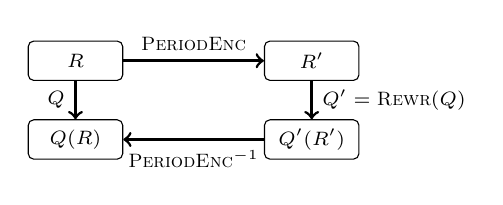
\begin{tikzpicture}[baseline=(current  bounding  box.center)]
    \tikzstyle{every node}=[font=\scriptsize]
    \node[draw, minimum width=1.2cm, minimum height=0.5cm,rounded corners=2pt] (R) {$\rel$}; %
    \node[draw, minimum width=1.2cm, minimum height=0.5cm,rounded corners=2pt] (Rp) at ($(R)+(3cm,0)$) {$\rel'$}; %
    \node[draw, minimum width=1.2cm, minimum height=0.5cm,rounded corners=2pt] (Q)  at ($(R)+(0,-1cm)$) {$\query(\rel)$}; %
    \node[draw, minimum width=1.2cm, minimum height=0.5cm,rounded corners=2pt] (Qp) at ($(R)+(3cm,-1cm)$) {$\query'(\rel')$}; %
    \draw[->, line width=1pt] (R) -- node[above]{$\reprN$} (Rp); %
    \draw[->, line width=1pt] (R) -- node[left]{$\query$} (Q); %
    \draw[->, line width=1pt] (Rp) -- node[right]{$\query'=\reprRewr(\query)$} (Qp); %
    \draw[->, line width=1pt] (Qp) -- node[below]{$\reprN^{-1}$} (Q); %
  \end{tikzpicture}
  \end{equation}
%\end{center}
%%%%%%%%%%%%%%%%%%%%%%%%%%%%%%%%%%%%%%%%

  Our encoding represents a tuple $\tuple$ annotated with a temporal element $\anyTE$ as a set of tuples, one for each interval $\interval$ which is assigned a non-zero value by $\anyTE$. For each such interval, the interval's end points are stored in two attributes $\attrBegin$ and $\attrEnd$, which are appended to the schema of $\tuple$.   Again, we use $\tuple \mapsto k$ to denote that tuple $\tuple$ is annotated with $k$ and $\valDom$ to denote a universal domain of values. We use
  $\schemaOf{R}$ to denote the schema of relation $R$ and
  $\arity(R)$ to denote its arity (the number of attributes in the schema).

%%%%%%%%%%%%%%%%%%%%%%%%%%%%%%%%%%%%%%%%
\begin{defi}[Encoding as SQL Period Relations]\label{def:N-enc}
 $\reprN$ is a function from $\semTimeNIN$-relations to $\semN$-relations.   Let $\rel$ be a $\semTimeNIN$ relation with schema $\schemaOf{\rel} = \{\attr_1, \ldots, \attr_n\}$. The schema of $\reprN(\rel)$ is $\{\attr_1, \ldots, \attr_n, \attrBegin, \attrEnd\}$.
  Let $\rel'$ be $\reprN(\rel)$ for some $\semTimeNIN$-relation.
  $\reprN$ and its inverse are defined as follows:
  \vspace{-3mm}
  \begin{align*}
    \reprN(R) &= \bigcup_{t \in \valDom^{\arity(R)}} \bigcup_{\interval \in \intervalDom} \{ (t, \iBegin{\interval}, \iEnd{\interval}) \mapsto R(t)(\interval) \}\\
    \reprN^{-1}(R') &= \bigcup_{t \in \valDom^{\arity(R)}} \{ t \mapsto \anyTE_{R',t} \}\\
  \forall \interval \in \intervalDom:  \anyTE_{R',t}(\interval) &= R'(\tuple_{\interval}) \mathtext{for} \tuple_{\interval} = (t, \iBegin{\interval}, \iEnd{\interval})
  \end{align*}
\end{defi}
%%%%%%%%%%%%%%%%%%%%%%%%%%%%%%%%%%%%%%%%

Before we define the rewriting $\reprRewr$ that reduces a query
$\query$ with $\semTimeNIN$ semantics to a query with $\semN$
semantics, we introduce two operators that we will make use of in the
reduction. The $\semN$-coalesce operator applies $\kCoalesce{\semN}$
to the annotation of each tuple in its input.

%%%%%%%%%%%%%%%%%%%%%%%%%%%%%%%%%%%%%%%%
\begin{defi}[Coalesce Operator]\label{def:coalesce-op}
Let $\rel$ be $\reprN(\rel')$ for some $\semTimeNIN$-relation $\rel'$.
The coalesce operator $\coalesceOp(\rel)$ is defined as:
% takes as input a $\semN$-relation $\rel$ that is an encoding of a $\semTimeNIN$-relation. % The operator return the encoding of the
  \begin{align*}
    \coalesceOp(R) &= \reprN(R')\\
  \forall \tuple: R'(t) &= \kCoalesce{\semN}(\reprN^{-1}(\rel)(t))
  \end{align*}
\end{defi}
%%%%%%%%%%%%%%%%%%%%%%%%%%%%%%%%%%%%%%%%

%%%%%%%%%%%%%%%%%%%%%%%%%%%%%%%%%%%%%%%%
\begin{figure*}[t]
  \centering
    \begin{align*}
%%%%%%%%%%%%%%%%%%%%
\underline{\reprRewr(R)} & = R & \underline{\reprRewr(\selection_\theta(\query))} &= \coalesceOp(\selection_\theta(\reprRewr(\query))) &
%%%%%%%%%%%%%%%%%%%%
\underline{\reprRewr(\projection_A(\query))} &= \coalesceOp(\projection_{A,\attrBegin, \attrEnd}(\reprRewr(\query))) &
    \end{align*}\\[-6mm]
    \begin{align*}
%%%%%%%%%%%%%%%%%%%%
    \underline{\reprRewr(\query_1 \join_\theta \query_2)} &= \coalesceOp(\projection_{\schemaOf{\query_1 \join_{\theta} \query_2}, max(\query_1.\attrBegin, \query_2.\attrBegin),min(\query_1.\attrEnd, \query_2.\attrEnd)} (\reprRewr(\query_1) \join_{\theta \wedge  overlaps(\query_1,\query_2)} \reprRewr(\query_2)))\\
%%%%%%%%%%%%%%%%%%%%
      \underline{\reprRewr(\query_1 - \query_2)} &= \coalesceOp(\normalizeOp_{\schemaOf{\query_1}}(\reprRewr(\query_1), \reprRewr(\query_2)) -  \normalizeOp_{\schemaOf{\query_2}}(\reprRewr(\query_2), \reprRewr(\query_1)))
%%%%%%%%%%%%%%%%%%%%
    \end{align*}\\[-7mm]
\revm{    \begin{align*}
            \underline{\reprRewr(\aggregation{}{f(A)}(\query))} &= \coalesceOp (\aggregation{\attrBegin, \attrEnd}{f(A)}(\normalizeOp_{\emptyset}(\reprRewr(\query) \union \{(null,\tMin, \tMax)\}, \reprRewr(\query))))\\[-1mm] %& %\underline{\reprRewr(\query_1 \union \query_2)} &= \coalesceOp(\reprRewr(\query_1) \union \reprRewr(\query_2)) \end{align*}\\[-6mm]                                                                                                                                                                                                                         \begin{align*}
            \underline{\reprRewr(\aggregation{}{count(*)}(\query))} &= \reprRewr(\aggregation{}{count(A)}(\projection_{1 \to A}(\query)))
%%%%%%%%%%%%%%%%%%%%
\end{align*}}\\[-7mm]
\begin{align*}
  \underline{\reprRewr(\aggregation{G}{f(A)}(\query))} &= \coalesceOp (\aggregation{G,\attrBegin, \attrEnd}{f(A)}(\normalizeOp_{G}(\reprRewr(\query), \reprRewr(\query))))
& %%%%%%%%%%%%%%%%%%%%
 \underline{\reprRewr(\query_1 \union \query_2)} &= \coalesceOp(\reprRewr(\query_1) \union \reprRewr(\query_2))
    \end{align*}\\ %[-5mm]
  \caption{Rewriting $\reprRewr$ that reduces queries over $\semTimeNIN$ to queries over a multiset encoding produced by $\reprN$.}
  \label{fig:rewrite}
\end{figure*}
%%%%%%%%%%%%%%%%%%%%%%%%%%%%%%%%%%%%%%%%


The split operator $\normalizeOp_{G}(R,S)$ splits the intervals in the
temporal elements annotating a tuple $\tuple$ based on the union of
all interval end points from annotations of tuples $\tuple'$ which
agree with $\tuple$ on attributes $G$. Inputs $R$ and $S$ have to be
union compatible. The effect of this operator is that all pairs of
intervals mapped to non-zero elements are either the same or are
disjoint. This operator has been applied
in~\cite{DignosBG12,DignosBGJ16} and in \cite{BowmanT03,T98}. We use
it to implement snapshot-reducible aggregation and difference over
intervals instead of single snapshots as in
Section~\ref{sec:complex-queries}. Recall that in Section~\ref{sec:complex-queries}, the monus (difference) and aggregation were defined in a point-wise manner. The split operator allows us to evaluate these operations over intervals directly by generating tuples with intervals for which the result of these operations is guaranteed to be constant.
%Recall that $\CPs{\anyTE}$ denotes the change points of a temporal element $\anyTE$.

%%%%%%%%%%%%%%%%%%%%%%%%%%%%%%%%%%%%%%%%
\begin{defi}[Split Operator]
  The split operator $\normalizeOp_G(R_1,R_2)$ takes as input two $\semN$-relations $R_1$ and $R_2$ that are encodings of $\semTimeNIN$-relations. For a tuple $\tuple$ in such an encoding let $\interval(\tuple) = [\tuple.\attrBegin, \tuple.\attrEnd)$. The split operator is defined as:
  \begin{align*}
    \normalizeOp_G(R_1,R_2)(\tuple) &= split(\tuple, R_1, EP_G(R_1 \cup R_2,t))\\
    EP_G(R,t) &= \bigcup_{t' \in R: t'.G = t.G \wedge R(t') > 0} \{t'.\attrBegin \} \cup \{t'.\attrEnd\}\\ %\\ & \cup \bigcup_{t' \in R_2: t'.G = t.G} \EPs{R_2(t')}\\
    split(\tuple, R, EP) &= \sum_{\tuple': \interval(\tuple) \subseteq \interval(\tuple') \wedge \interval(\tuple) \in EPI(t, EP)} R(\tuple')\\
    EPI(t, EP) &= \{ [\tPoint_b , \tPoint_e) \mid  \tPoint_b \tLe \tPoint_e \wedge \tPoint_b \in EP \wedge\\ &\mathtab\mathtab(\tPoint_e  \in EP \vee T_e = \tMax) \wedge\\ &\mathtab\mathtab \not\exists \tPoint' \in EP: \tPoint_b \tLe \tPoint' \tLe \tPoint_e \}
  \end{align*}
\end{defi}
%%%%%%%%%%%%%%%%%%%%%%%%%%%%%%%%%%%%%%%%

The use of the $\reprN$ and $\reprN^{-1}$ mappings in the definitions of the coalesce and split algebra operators is only for ease of presentation. These  operators can be implemented as SQL queries executed over an $\reprN$-encoded relation.

%%%%%%%%%%%%%%%%%%%%%%%%%%%%%%%%%%%%%%%%
\begin{defi}[Query Rewriting]\label{def:repr-N-rewriting}
  % We define a representation system  $(\repr, \repr^{-1}, \reprRewr)$ to encode a $\semTimeNI$-database as a $semN$-database. We define $\repr$ and $\repr^{-1}$ for single relations, the application of $\repr$ to a database is defined as the result of applying $\repr$ to each relation of the database. Let $R$ be a $\semTimeNI$ relation and $R'$ denote an  $\semN$ encoding a $\semTimeNI$ relation, i.e., $R' = \repr(R)$ for some $R$.
  % We assume that the additional attributes of a representation $R'$ that store intervals are called $\attrBegin$ and $\attrEnd$.
We use $overlaps(\query_1, \query_2)$ as a % notational
shortcut for
$\query_1.\attrBegin < \query_2.\attrEnd \land \query_2.\attrBegin < \query_1.\attrEnd$.
  The definition of rewriting $\reprRewr$ is shown in Figure~\ref{fig:rewrite}.
  % \begin{align*}
  %   \reprRewr(\selection_\theta(\query)) &= \coalesceOp(\selection_\theta(\reprRewr(\query)))\\
  %   \reprRewr(\projection_A(\query)) &= \coalesceOp(\projection_{A,\attrBegin, \attrEnd}(\reprRewr(\query)))\\
  %   \reprRewr(\query_1 \union \query_2) &= \coalesceOp(\reprRewr(\query_1) \union \reprRewr(\query_2))\\
  %   \reprRewr(\query_1 \join_\theta \query_2) &= \coalesceOp(\\
  %                                               &\hspace{-2cm}\projection_{\schemaOf{\query_1 \join_{\theta} \query_2}, max(\query_1.\attrBegin, \query_2.\attrBegin), min(\query_1.\attrEnd, \query_2.\attrEnd)} (\\
  %                                        &\hspace{-1.5cm}\reprRewr(\query_1) \join_{\theta \wedge  overlaps(\query_1,\query_2)} \reprRewr(\query_2)))\\
  %   \reprRewr(\query_1 - \query_2) &= \coalesceOp(\normalizeOp_{\schemaOf{\query_1}}(\reprRewr(\query_1), \reprRewr(\query_2))\\ &-  \normalizeOp_{\schemaOf{\query_2}}(\reprRewr(\query_2), \reprRewr(\query_1)))\\
  %   \reprRewr(\aggregation{G}{aggr}(\query)) &= \coalesceOp (\aggregation{G,\attrBegin, \attrEnd}{aggr}(\normalizeOp_{G}(\reprRewr(\query) \union \{(\neutralAggr)\}, \reprRewr(\query))))
  % \end{align*}
Here % $\neutralAggr$ denote the result of an aggregation function over an empty input ($\aNeutralAggr{count} = 0$ and $\aNeutralAggr{a} = null$  for any other aggregation function $a$) and
$\{t\}$ denotes a constant relation with a single tuple $t$ annotated with $1$.
\end{defi}
%%%%%%%%%%%%%%%%%%%%%%%%%%%%%%%%%%%%%%%%

Note that the rule for $count(*)$ is a necessary preprocessing step that takes precedence over the rule for general aggregation. % It is a pre-processing step necessary to ensure correctness of the rewriting.

\revm{
%%%%%%%%%%%%%%%%%%%%%%%%%%%%%%%%%%%%%%%%
\begin{exam}\label{ex:rewriting}
  Reconsider query $\qAggEx$ from Example~\ref{ex:running-example-snapshot} and its results for the logical model and period relations (Figure~\ref{fig:overview-approach}). % We now explain how to apply $\reprRewr$ to generate the query producing the SQL period encoding.
  In relational algebra, the input query is written as $\qAggEx = \aggregation{}{count(*)} (\underbrace{\selection_{skill=SP}(works)}_{\query_1})$. Applying $\reprRewr$ we get:
%
  \begin{align*}
\reprRewr(\qAggEx) &=
                    \coalesceOp (\aggregation{\attrBegin, \attrEnd}{count(A)}(\normalizeOp_{\emptyset}(\\
    &\hspace{-1mm}\projection_{1 \to A, \attrBegin, \attrEnd}(\reprRewr(\query_1)) \union \{(null,0, 24)\},\\ &\hspace{-1mm}\reprRewr(\query_1))))\\
\reprRewr(\query_1) &= \coalesceOp(\selection_{skill=SP}(works))
  \end{align*}
  Subquery $\reprRewr(\query_1)$  filters out the second tuple from the input (see Figure~\ref{fig:overview-approach}). The split operator is then applied to the union of the result of $\reprRewr(\query_1)$ and a tuple with the neutral element $null$ for the aggregation function and period $[\tMin, \tMax)$, where $\tMin = 0$ and $\tMax = 24$ for this example.
%
After the split $\normalizeOp$, the aggregation is evaluated grouping the input on $\attrBegin, \attrEnd$. The \lstinline!count! aggregation function then either counts a sequence of $1$s and a single  $null$ value producing the number of facts that overlap over the corresponding period $[\attrBegin, \attrEnd)$, or counts a single $null$ value over a ``gap'' producing $0$.
For instance, for $[08,10)$ there are two facts whose intervals cover this period (Ann and Sam) and, thus, $(2, [08,10))$ is returned by $\reprRewr(\qAggEx)$. While for for $[20,24)$ there are no facts and thus we get $(0, [20,24))$.
%
% each ``gap'' is covered by an interval assigned
% $null$ and for every tuple with multiplicity $m$ in the input there will be $m$ duplicates assigned value $1$ for every pair of interval end time points that are covered by the period of the tuple. Then the aggregation is evaluated grouping the input on $\attrBegin, \attrEnd$ computing the \lstinline!count!, resulting in $0$ for $null$ values and $m$ for $m$ duplicates. For example, for the adjacent endpoints $[08,10)$, there are two tuples whose intervals cover this period (employees Ann and Sam) and, thus, $(2, [08,10))$ is returned by $\reprRewr(\qAggEx)$.
\end{exam}
%%%%%%%%%%%%%%%%%%%%%%%%%%%%%%%%%%%%%%%%
}
% The following theorem shows that the commutative diagram from Equation~\eqref{eq:n-enc-cd} is correct.

%%%%%%%%%%%%%%%%%%%%%%%%%%%%%%%%%%%%%%%%
\begin{theo}\label{theo:reduction-is-correct}
The commutative diagram in Equation~~\eqref{eq:n-enc-cd} holds.
\end{theo}
%%%%%%%%%%%%%%%%%%%%%%%%%%%%%%%%%%%%%%%%
\proofsketch{\revm{
Proven by induction over query structure.
    }}
% \BG{
%   \textbullet Certain operators perserve coalescing (compare to Michaels set-coalescing optimizations). This means we can sometimes push down the coalesce (are there any situations where we want to do that though?)
%   \textbullet Normalization optimization refer to Toman~ (cite{BT03})
%   \textbullet Combine Normalize with set diff or aggregation into one, hopefully, more efficient rewrite
% }

%%%%%%%%%%%%%%%%%%%%%%%%%%%%%%%%%%%%%%%%%%%%%%%%%%%%%%%%%%%%%%%%%%%%%%%%%%%%%%%%
\section{Implementation}
\label{sec:implementation}

We have implemented the encoding and rewriting introduced in the
previous section in a middleware which supports snapshot multiset
semantics through an extension of SQL. To instruct the system to
interpret a subquery using snapshot semantics, the user encloses the
subquery in a \texttt{SEQ VT (...)} block. We assume that the inputs
to a snapshot query are encoded as period multiset relations, i.e.,
each relation has two temporal attributes that store the begin and end
timestamp of their validity interval. For each relation access within
a \texttt{SEQ VT} block, the user has to specify which attributes
store the period of a tuple. \BGDel{We choose to implement this
  middleware as an extension of the GProM system to benefit from the
  system's support for multiple database backends.}{we should not
  mention GProM anyways because of double blind and here it is not
  important that this is build based on GProM}

%\BG{In case we do use the optimizer: Furthermore, the built-in optimizer enabled us to make cost-based decisions about \ldots}

% \BG{Not sure we will need that}

Our coalescing and split operators can be expressed in SQL. Thus, a
straightforward way of incorporating these operators into the
compilation process is to devise additional rewrites that produce the
relational algebra code for these operators where necessary. However,
preliminary experiments demonstrated that a naive implementation of
these operators is prohibitively expensive. \BGDel{ increasing the query
execution time by several orders of magnitude compared to non-temporal
queries in some cases.}{space}

We address this problem in two ways. First, we observe that it is sufficient to apply coalesce as a last step in a query instead of applying it as part of every operator rewrite. Applying this optimization, the rewritten version of a query will only contain one coalesce operator. Recall from Lemma~\ref{lem:coalesce-push} that coalescing can be redundantly pushed into the addition and multiplication operations of period semirings, e.g., $\kCoalesce{\semK}(k \addP k') = \kCoalesce{\semK}(\kCoalesce{\semK}(k) \addP k')$.
\ifnottechreport{We have proven that this Lemma also holds for monus~\cite{DG18}.}
\iftechreport{We prove that this Lemma also holds for monus in Appendix~\ref{sec:optimizations}.}
Interpreting this equivalence from right to left and applying it repeatedly to a semiring expression $e$, $e$ can be rewritten into an equivalent expression of the form $\kCoalesce{\semK}(e')$, where $e'$ is an expression that only uses operations $\addP$, $\multP$, and $\monP$. Since relational algebra over K-relations is defined by applying multiplication, addition, and monus to input annotations, this implies that it is sufficient to apply coalescing only as a final operation in a query. \iftechreport{For an example and additional discussion see Appendix~\ref{sec:optimizations}}\ifnottechreport{For further discussion of this optimization and an example see~\cite[Appendix C]{DG18}.}


We developed an optimized implementation of multiset coalescing using SQL
analytical window functions\reva{, similar to set-based coalescing
in~\cite{ZhouWZ06}}, that counts \reva{for value-equivalent attributes} the
number of open intervals per time point, determines change points based on
differences between these counts, and then only output maximal intervals using
a filter step. \reva{This implementation uses sorting in its window declarations % based on
% sorting
and has time complexity $\mathcal{O}(n \log{n})$ for $n$ tuples.
A native implementation would require only one sorting step. The number of sorting steps required by our SQL implementation depends
on whether the DBMS is capable of sharing window declarations (we observe 2 and 7 sorting steps for the systems used in our experimental evaluation).}

\reva{For aggregation we integrate the split operator into the
aggregation. It turned out to be most effective to pre-aggregate the input
before splitting and then compute the final aggregation results during the
split step by further aggregating the results of the pre-aggregation step.} We apply a similar optimization for difference.

% Consider how a $\raPlus$ query $\query$ is evaluated over an $\semTimeNI$-database. $\raPlus$ over K-relations computes the annotation of a tuple in the result of a query using the addition and multiplication operations of the semiring. That is, the annotation of any result tuple is computed using an arithmetic expression over the annotations of tuples from the input of the query. In the case of a semiring $\semTimeNI$, addition and multiplication are defined as coalescing a temporal element that is computed based on point-wise application of the addition (multiplication) operations of semiring $\semK$ (denoted as $\addP$ and $\multP$).
% Recall from Lemma~\ref{lem:coalesce-push} that coalescing can be redundantly pushed into the addition and multiplication operations of interval-temporal semirings, e.g., $\kCoalesce{\semK}(k \addP k') = \kCoalesce{\semK}(\kCoalesce{\semK}(k) \addP k')$. Interpreting this equivalence from right to left and applying it repeatedly to an arithmetic expression $e$ using $\addNI$ and $\multNI$, the expression can be rewritten into an equivalent expression of the form $\kCoalesce{\semK}(e')$, where $e'$ is an expression that only uses operations $\addP$ and $\multP$. Now consider expressions that also include applications of the monus operator $\monNI$. This operator is defined as $\kCoalesce{\semK}(k \monP k')$. The $\monP$ operator computes the timeslice of the inputs at every point in time and then applies $\monK$ to each timeslice. According to Lemma~\ref{lem:coalesce-properties}, $\tSlice{\tPoint}(k) \intervalEq \tSlice{\tPoint}(\kCoalesce{\semK}(k'))$. Thus, the result of $\monP$ is independent of whether the input is coalesced or not.

% %%%%%%%%%%%%%%%%%%%%%%%%%%%%%%%%%%%%%%%%
% \begin{lem}\label{lem:single-coalesce-enough}
% Any arithmetic expression $e$ using operations and elements from an interval-temporal m-semiring $\semTimeNI$ is equivalent to an expression of the form $\kCoalesce{\semK}(e')$, where $e'$ only contains operations $\addP$, $\multP$, and $\monP$.
% \end{lem}
% %%%%%%%%%%%%%%%%%%%%%%%%%%%%%%%%%%%%%%%%

% Lemma~\ref{lem:single-coalesce-enough} implies that it is sufficient to apply coalescing as a last step in a rewritten query $\reprRewr(\query)$ instead of after each operator.   % to the input of these operations if the output of the operation is also subjected to coalescing.
% % Since positive relational algebra over K-relations is defined using addition and multiplication,
% % Thus, for any $\raPlus$ query $\query$ it is sufficient to apply coalescing as a last step instead of after each relational algebra operation.

% %%%%%%%%%%%%%%%%%%%%%%%%%%%%%%%%%%%%%%%%
% \begin{coll}[Coalesce Pullup]\label{coll:coalesce-pullup}
%   For any $\ra$ query $\query$, $\reprRewr(\query)$ is equivalent to a query $\query'$ which is derived from $\reprRewr(\query)$ by removing all but the outermost coalescing operator.
% \end{coll}
% %%%%%%%%%%%%%%%%%%%%%%%%%%%%%%%%%%%%%%%%



% A detailed experimental comparison of different
% algorithms that implement these operators and an implementation of
% these algorithms in a database kernel is beyond the scope of this
% work. Here we settled for using optimized implementations of these
% operators in SQL. For coalescing we use analytical functions to count
% the number of open intervals per time point, use these counts to
% determine change points, and then only output maximal intervals using
% a filter step.  For splitting aggregation inputs, it turned out to be
% most effective to pre-aggregate the input and then compute the final
% aggregation results during the split step. We apply a similar
% optimization for difference.
%\BG{Integrate this above? we develop a more effective SQL implementation of coalescing using analytical functions (SQL's \lstinline!OVER! clause).}
% %%%%%%%%%%%%%%%%%%%%%%%%%%%%%%%%%%%%%%%%%%%%%%%%%%%%%%%%%%%%%%%%%%%%%%%%%%%%%%%%
% \section{Infinite and Contigous Temporal Domains}
% \label{sec:infin-cont-temp}

% \BG{Add discussion on this here? Too much?}

%%%%%%%%%%%%%%%%%%%%%%%%%%%%%%%%%%%%%%%%%%%%%%%%%%%%%%%%%%%%%%%%%%%%%%%%%%%%%%%%
\section{Experiments}
\label{sec:experiments}

In our experimental evaluation we focus on two aspects. First, we
evaluate the cost of our SQL implementation of $\semN$-coalescing
(multiset coalescing).  Then, we evaluate the performance of snapshot
queries with our approach over three DBMSs and compare it against
native implementations of snapshot semantics that are available in
two of these systems (using our implementation of coalescing to
produce a coalesced result).

%%%%%%%%%%%%%%%%%%%%%%%%%%%%%%%%%%%%%%%%%%%%%%%%%%%%%%%%%%%%
\subsection{Workloads and Experimental Setup}
\label{sec:data-sets}

%%%%%%%%%%%%%%%%%%%%%%%%%%%%%%%%%%%%%%%%
\parttitle{Datasets} We use \reva{\iftechreport{three}\ifnottechreport{two} datasets in our experiments}. The \textit{MySQL Employees dataset}
(\url{https://github.com/datacharmer/test_db})
 which contains
$\approx$4~million records and consists of the following six
period tables: table \texttt{employee} stores basic information about
employees; table \texttt{departments} stores department information;
table \texttt{titles} stores the job titles for employees; table
\texttt{salaries} stores employee salaries; table
\texttt{dept\_manager} stores which employee manages which
department; and table \texttt{dept\_emp} stores which employee is
working for which department.
\reva{\textit{TPC-BiH} is the bi-temporal version of the TPC-H benchmark dataset as described in~\cite{DBLP:conf/tpctc/KaufmannFMTK13}. Since our approach supports only one time dimension we only generated the valid time dimension for this dataset. In this configuration a scale factor 1 (SF1) database corresponds to roughly 1GB of data.}
\ifnottechreport{
\reva{In our technical report we also use a real-world \textit{Tourism} dataset (835k records).}
}
\iftechreport{
The \textit{Tourism} dataset (835k records) consists of a single table storing hotel reservations in South Tyrol. Each record corresponds to one reservation. The validity end points of the time period associated with a record is the arrival and departure time.
}


%%%%%%%%%%%%%%%%%%%%%%%%%%%%%%%%%%%%%%%%
\parttitle{Workloads}
\ifnottechreport{To evaluate the efficiency of snapshot queries, we
  created a workload consisting of the following 10 queries expressed over the employee dataset. \texttt{join-1}:
  salary and department for each employee using a join
  between the department and salary tables. \texttt{join-2}:
  salary and title for each employee using a join between the
  salary and title tables.  \texttt{join-3}:
  department of employees that manage a department and earn more than
  \$70,000 using a join between the manager and salary tables and a
  selection on attribute salary.\texttt{join-4}: gather all information for each manager using joins
  between the tables managers, salary, and employees.
  \texttt{agg-1}: average salary of employees per
  department using the result of query \texttt{join-1} with a
  subsequent aggregation per department. \texttt{agg-2}:
  average salary of managers using a join between the
  manager and salary tables with a subsequent aggregation without
  grouping. \texttt{agg-3}: number of departments
  with more than 21 employees. This query has no join but two
  aggregations, one to compute the number of employees per department
  and a second one to count the number of relevant departments.
  \texttt{agg-join}: names of employees with the highest
  salary in their department.  This query consists of a 4-way join where one
  of the inputs is the result of a subquery with aggregation.
  \texttt{diff-1}: employees that are not managers using a
  difference operation between two tables.  \texttt{diff-2}:
  salaries of employees that are not managers by computing
  the difference between a table and a subquery with a join.
  %
  % Furthermore, we use one query template varying the selectivity to
  % evaluate
  % the performance of coalescing. The query returns employees that
  % earn
  % more than a specific salary. \texttt{C-Sn} denotes an
  % instantiation of this query
  % that returns approximately $n \cdot 10^3$ rows, e.g.,
  % \texttt{C-S1} returns 1,000 rows.
  \reva{
    For the TPC-BiH dataset we took 9 of the 22 standard queries~\cite{tpc-h} from this benchmark that do not contain nested subqueries or \lstinline!LIMIT! (which are not supported by our or any other approach for snapshot queries we are aware of) and evaluated these queries under snapshot semantics. Note that some of these queries use the \lstinline!ORDER BY! clause that we do not support for snapshot queries. However, we can evaluate such a query without \lstinline!ORDER BY! under snapshot semantics and then sort the result without affecting what rows are returned.
      % \texttt{agg-join}: number of enquiries per continent. This query first join tourismdata and country tables and do an aggregation on it.
  }
  The number of rows returned by the \reva{Employee and TPC-H}  queries are
  shown in Table~\ref{tab:query-result}. The SQL code and more detailed descriptions of \reva{these} queries are provided in~\cite[Appendix B]{DG18}.
}
\iftechreport{
  We have created a workload consisting of 10 queries to evaluate the
  efficiency of snapshot queries. Queries \texttt{join-1} to \texttt{join-4}
  are join queries, \texttt{agg-1} to \texttt{agg-3} are aggregation-heavy
  queries, \texttt{agg-join} is a join with an aggregation value, and
  \texttt{diff-1} and \texttt{diff-2} use difference. Furthermore, we use one
  query template varying the selectivity to evaluate the performance of
  coalescing. \texttt{C-Sn} denotes the variant of this query that returns
  approximately $nK$ rows, e.g., \texttt{C-S1} returns 1,000 rows.
For the Tourism dataset we use the following queries. \texttt{join}: tourist from same country to same destination using a self join of tourismdata table.  \texttt{agg-0}: number of tourists per destination together with the average number of tourists for all other destinations. This query first computes the number of tourists per destination and do a self unequal join on it. \texttt{agg-1}: number of enquiries and the number of tourists per destination with more than 1000 enquiries using two aggregations on tourismdata table. \texttt{agg-2}: maximum number of tourists per destination using an aggregation on tourismdata table. \texttt{tou-agg-x}: the destination with the most number of tourists. This query has no join but two aggregations, one to compute the number of tourists per destination and a second one to compute the maximum one.
  More
  detailed descriptions of these queries are provided in
  Appendix~\ref{sec:workload-queries}.
    For the TPC-BiH dataset we took 9 of the 22 standard queries~\cite{tpc-h} from this benchmark that do not contain nested subqueries or \lstinline!LIMIT! (which are not supported by our or any other approach for snapshot queries we are aware of) and evaluated these queries under snapshot semantics. Note that some of these queries use the \lstinline!ORDER BY! clause that we do not support for snapshot queries. However, we can evaluate such a query without \lstinline!ORDER BY! under snapshot semantics and then sort the result without affecting what rows are returned.
  The number of rows returned by these
  queries over the  dataset are shown in Table~\ref{tab:query-result}.
}

%%%%%%%%%%%%%%%%%%%%%%%%%%%%%%%%%%%%%%%%
\begin{table}[thb]
  \caption{Number of query result rows}
  \label{tab:query-result}
\centering
\resizebox{1\columnwidth}{!}{
\setlength{\tabcolsep}{3pt}
\begin{minipage}{1.4\linewidth}
\centering
\begin{tabular}[t]{|r|r|r|r||r|r|r||r||r|r|}
 \hline
 \thead{join-1} &   \thead{join-2} &    \thead{join-3}  & \thead{join-4} & \thead{agg-1}  & \thead{agg-2}  &
\thead{agg-3}  &  \thead{agg-join} &   \thead{diff-1} &  \thead{diff-2}
\\ \hline
  2.8M & 28.3M  & 10 &  177 &  57.4k & 177 & 210 & 260 & 300k  &  2.8M
  \\ \hline
\end{tabular}\\[2mm]
\reva{
\begin{tabular}[t]{|c|c|c|c|c|c|c|c|c|c|c|c|}
  \hline
 \thead{TPC-H}& \thead{Q1} & \thead{Q3} & \thead{Q5} & \thead{Q6} & \thead{Q7} & \thead{Q8} & \thead{Q9} & \thead{Q10} & \thead{Q12} & \thead{Q14} & \thead{Q19} \\ \hline
 \thead{1GB} & 4.3k & 10 & 386 & 529 & 1.6k & 742 & 69.7k & 20 & 785 & 479 & 220 \\ \hline
 \thead{10GB} & 4.3k & 10 & 579 & 532 & 1.7k & 867 & 74.8k & 20 & 786 & 487 & 1.3k \\ \hline
\end{tabular}\\[2mm]
}
\iftechreport{
\reva{
\begin{tabular}[t]{|r||r|r|r||r|}
 \hline
 \thead{tou-join-agg} &   \thead{tou-agg-1} &   \thead{tou-agg-2} & \thead{tou-agg-3}  & \thead{tou-agg-join}
\\ \hline
 64.3k & 954  & 14.5k &  3.2k &  822
  \\ \hline
\end{tabular}
}
}
\end{minipage}
}
\end{table}
%%%%%%%%%%%%%%%%%%%%%%%%%%%%%%%%%%%%%%%%


%%%%%%%%%%%%%%%%%%%%%%%%%%%%%%%%%%%%%%%%
% \begin{figure}[t]
%   \centering
%   \includegraphics[width=0.8\linewidth,trim=10pt 30pt 0 130pt, clip]{figs/coalesce-selectivity.pdf}
%   \caption{Multiset coalescing for varying input size.}
%   \label{fig:coalesce-selectivity}
% \end{figure}
%%%%%%%%%%%%%%%%%%%%%%%%%%%%%%%%%%%%%%%%

% \begin{figure}[htb]
% \begin{tabular}{l|p{5.5cm}}
%   \thead{query} & \thead{description} \\
%   \texttt{join-1} & salary and department for each employee using a join
%   between departments and salaries tables. \\
%   \hline
%   \texttt{join-2} & salary and title for each employee using a join between
%   salaries and titles tables. \\
%   \hline
%   \texttt{join-3} & department of employees that manage a department and earn
%   more than \$70,000 using a join between managers and salary table with a
%   section on the salary. \\
%   \hline
%   \texttt{join-4} & join between three tables and returns the full information
%   of each manager using joins between the tables managers, salary, and
%   employees. \\
%   \hline
%   \texttt{agg-1} & average salary of employees per department using the join of
%   query \texttt{join-1} with a subsequent aggregation per department. \\
%   \hline
%   \texttt{agg-2} & average salary of managers using a join between managers and
%   salary tables with a subsequent aggregation without grouping.\\
%   \hline
%   \texttt{agg-3} & number of departments with more than 21 employees. This
%   query has no join but two aggregations, one to compute number of employees
%   per department and a second to count the number of relevant departments.\\
%   \hline
%   \texttt{agg-join} & names of employees with the highest salary in their
%   department. It contains a 4-way join where one of the inputs is the result of
%   a subquery with aggregation. \\
%   \hline
%   \texttt{diff-1} & employees that are not managers using a difference
%   operation between two tables.\\
%   \hline
%   \texttt{diff-2} & salaries of employees that are not managers. It
%   contains a difference between a table and a subquery with a join.\\
%   \hline
% \end{tabular}
% \caption{Query Workloads.\AD{Tried to make it a table.}}
% \label{fig:queries}
% \end{figure}


%%%%%%%%%%%%%%%%%%%%%%%%%%%%%%%%%%%%%%%%
% \begin{figure*}[t]
%   \centering
%
%   \begin{tabular}{|l|rrrr|rrr|r|rr|}\hline
%     \thead{System} & \thead{join-1} & \thead{join-2} & \thead{join-3} & \thead{join-4} & \thead{agg-1} & \thead{agg-2} & \thead{agg-3} & \thead{agg-Join} & \thead{diff-1} & \thead{diff-2}\\ \hline
% Postgres-Seq &    91.9708 &  1543.8150  &0.0126  &0.5224  &7.0180  &0.0570  &  1.4240 &6643.6110  &14.1755  &63.5803\\
% Postgres-Native & 118.0690 &888.1250 & 4.9093 & 12.8538 &5980.8490 &10.3050 &0.0200 &19195.0270 &6.8770 &79.6320\\ \hline
% DB-X-Seq &118.9540 & 1569.4540 &  0.5510 & 0.8300 & 56.4730 & 0.8180 & 0.7750 & \textcolor{red}{\textbf{OOTS}} & 30.1540 & 129.8700\\
% %DB-X-Native & 2.6010 &4.2150 &0.1830 &0.2590 &1200.0000 &0.4310 &0.2730 &3.8300 & N/A & N/A\\ \hline
% DB-X-Native & 116.0290 & 1200.3670 &0.4310 &0.5970 & \OOTS % 2350.5990+
%                                                                                                        &0.8180 &0.5470 & \OOTS & \ONA & \ONA\\ \hline
%     DB-Y-Seq & 64.0000 &763.6985 &0.0075 &0.2150 &5.2379 &0.0098 &0.0123 &7555.9661 &10.2853 &61.8972\\
%     \hline
%   \end{tabular}
%   \caption{Runtimes (sec) of Snapshot Queries: \ONA\, = not supported, \OOTS\, = system ran out of temporary space (2GB)}
%   \label{fig:runtime-seq-queries}
% \end{figure*}
% \subsection{Setup and Compared Methods}
%\label{sec:setup}

%%%%%%%%%%%%%%%%%%%%%%%%%%%%%%%%%%%%%%%%
\parttitle{Systems}
%
We ran experiments on three different database management systems: a
version of Postgres (\textit{PG}) with native support for temporal
operators as described in~\cite{DignosBG12,DignosBGJ16}; a commercial
DBMS, \textit{DBX}, with native support for snapshot semantics (only
available as a virtual machine); and a commercial DBMS, \textit{DBY},
without native support for snapshot semantics.
%
We used our approach to translate snapshot queries into standard SQL
queries and ran the translated queries on all three systems (denoted
as \textit{PG-Seq}, \textit{DBX-Seq}, and \textit{DBY-Seq}).
For PG and DBX, we ran the queries also with the native
solution for snapshot semantics paired with our implementation of
coalescing to produce a coalesced result (referred to as
\textit{PG-Nat} and \textit{DBX-Nat}).
%
As explained in Section~\ref{sec:related-work}, no system correctly
implements snapshot multiset semantics for difference and
aggregation, and many systems do not support snapshot semantics for
these operators at all. \textit{DBX-Nat} and \textit{PG-Nat}
both support snapshot aggregation, however, their implementations are
not snapshot-reducible. \textit{DBX-Nat} does not support snapshot difference,
whereas \textit{PG-Nat} implements temporal difference with set
semantics.  Despite such differences, the experimental comparison
allows us to understand the performance impact of our provably correct
approach.

All experiments were executed on a machine with 2 AMD Opteron 4238 CPUs, 128GB
RAM, and a hardware RAID with 4 $\times$ 1TB 72.K HDs in RAID 5. \revm{For Postgres we set the buffer pool size to $8$GB. For the other systems we use values recommended by the automated configuration tools of these systems. % values for our machine for the .
%
We execute
queries with warm cache. For short-running queries we show the median runtime
across 100 consecutive runs. For long running queries we computed the
median over 10 runs. In general we observed low variation in runtimes (a few
percent).}

%%%%%%%%%%%%%%%%%%%%%%%%%%%%%%%%%%%%%%%%%%%%%%%%%%%%%%%%%%%%%%%%%%%%%%%%%%%%%%%%
%\subsection{Performance Results}


\subsection{Multiset Coalescing}
\label{sssec:multiset-coalescing}

To evaluate the performance of coalescing, we use a selection query
that returns employees that earn more than a specific salary and
materialize the result as a table.  The selectivity varies from 1K to
3M rows.  We then evaluate the query \texttt{\textbf{SELECT} *
  \textbf{FROM} ...}  over the materialized tables under snapshot
semantics in order to measure the cost of coalescing in isolation.
Figure~\ref{fig:coalesce-selectivity} shows the results of this
experiment.  The runtime of coalescing is linear in the input size for
all three systems.  Even though the theoretical worst-case complexity
of the sorting step, which is applied by all systems to evaluate the
analytics functions that we exploit in our SQL-based implementation of
multiset coalescing, is $\mathcal{O}(n \cdot log (n))$, an inspection
of the execution plans revealed that the sorting step only amounts to
5\%-10\% of the execution time (for all selectivities) and, hence, is
not a dominating factor.

%%%%%%%%%%%%%%%%%%%%%%%%%%%%%%%%%%%%%%%%
\begin{figure}[t]
  \centering
  \includegraphics[width=0.8\linewidth,trim=10pt 30pt 0 130pt, clip]{../plot-scripts/coalesce-selectivity.pdf}
  \caption{Multiset coalescing for varying input size.}$\,$\\[1mm]
  \label{fig:coalesce-selectivity}
\end{figure}
%%%%%%%%%%%%%%%%%%%%%%%%%%%%%%%%%%%%%%%%


%%%%%%%%%%%%%%%%%%%%%%%%%%%%%%%%%%%%%%%%%%%%%%%%%%%%%%%%%%%%%%%%%%%%%%%%%%%%%%%%
\subsection{Snapshot Semantics  - Employee}
\label{sssec:sequ-semant-quer}

Table~\ref{tab:runtime-seq-queries} provides an overview of the
performance results for our snapshot query workloads. \revm{For every query we indicate in the rightmost column whether native approaches are subject to the aggregation gap (AG) or bag difference (BD) bugs.}

%%%%%%%%%%%%%%%%%%%%%%%%%%%%%%%%%%%%%%%%
\begin{table}[t]
  \caption{Runtimes (sec) of snapshot queries: \ONA\, = not supported, \OOTS\, = system ran out of temporary space (2GB), \TimeOut  = timed out (2 hours).}
  \label{tab:runtime-seq-queries}
  \centering
  \scriptsize
  \setlength{\tabcolsep}{3pt}
  \begin{tabular}{|l|rr|rr|r|c|}\hline
      \multicolumn{7}{|c|}{\textbf{Employee dataset}}\\
    \hline
   \thead{Query} & \thead{PG-Seq} & \thead{PG-Nat} & \thead{DBX-Seq} & \thead{DBX-Nat} & \thead{DBY-Seq} & \thead{Bug}\\ \hline
   \texttt{join-1} & 91.97 & 118.01 & 118.95 & 116.03 & 64.00 & \\
    \texttt{join-2} & 1543.81 & 888.13 & 1569.45 & 1200.36 & 763.70 &\\
   \texttt{join-3} & 0.01 & 4.91 & 0.55 & 0.43 & 0.01 & \\
   \texttt{join-4} & 0.52 & 12.85 & 0.83 & 0.60 & 0.22 & \\
   \hline
   \texttt{agg-1} & 7.02 & 5980.85 & 56.47 & \OOTS & 5.24 & \\
   \texttt{agg-2} & 0.06 & 10.31 & 0.82 & 0.82 & 0.01 & AG\\
   \texttt{agg-3} & 1.42 & 0.02 & 0.78 & 0.55 & 0.01 & AG\\
   \hline
   \texttt{agg-join} & 6643.61 & 19195.03 & \OOTS &  \OOTS & 7555.97 & \\
   \hline
   \texttt{diff-1} & 14.18 & 6.88 & 30.15 & \ONA & 10.29 &BD\\
   \texttt{diff-2} & 63.58 & 79.63 & 129.87 & \ONA & 61.90 &BD\\
    \hline \end{tabular}\\[3mm] %\hline
%%%%%%%%%%%%%%%%%%%%%%%%%%%%%%%%%%%%%%%%
\iftechreport{
  \reva{
  \begin{tabular}{|l|rr|r|c|}\hline
    \multicolumn{5}{|c|}{\textbf{Tourism}} \\ \hline
    \thead{Query} & \thead{PG-Seq} &  \thead{PG-Nat} &   \thead{DBY-Seq}  &  \thead{Bug}\\
    \hline
  \texttt{tou-join-agg} & 300.28 & 694.88 & 171.09 &  \\
  \hline
        \texttt{tou-agg-1} & 2.41 & 94.58 & 1.61 &  \\
        \texttt{tou-agg-2} & 123.79 & 92.32 & 87.31 &  \\
      \texttt{tou-agg-3} & 6.68 & 98.07 & 7.66 & AG \\
    \hline
        \texttt{tou-agg-join} & 1.06 & 263.61 & 0.94 &  \\
    \hline
  \end{tabular}\\[3mm]
}
}
  %%%%%%%%%%%%%%%%%%%%%%%%%%%%%%%%%%%%%%%%
   \reva{
     \begin{tabular}{|l|rrr|rrr|c|}\hline
     \multicolumn{8}{|c|}{\textbf{TPC-BiH}}\\ \hline
     &\multicolumn{3}{c|}{\textbf{SF1 ($\sim$1 GB)}} & \multicolumn{3}{c|}{\textbf{SF10 ($\sim$10 GB)}} & \\ \cline{2-7}
     \thead{Query} & \thead{PG-Seq} & \thead{PG-Nat} & \thead{DBY-Seq} & \thead{PG-Seq} & \thead{PG-Nat} & \thead{DBY-Seq} & \thead{Bug}\\
     \hline
\texttt{Q1} & 12.02 & 3686.47 &11.80 & 63.85 & \TimeOut & 82.61&\\
%\texttt{Q3} & 1.97 & 70.68 &2.49 &     21.72 & 814.60 & 21.38&\\ % top 10!!!!
\texttt{Q5} & 0.58 & 142.91 &1.14 &    5.85 & 1794.10 & 14.89&\\
\texttt{Q6} & 0.79 & 12.65 &1.14  &     7.70 & 126.91 & 7.28& AG\\
\texttt{Q7} & 1.14 & 285.91 &5.33&     28.70 & 1642.20 & 21.75&\\
\texttt{Q8} & 1.77 & 108.63 &2.20&     21.78 & 1484.61 & 17.33&\\
\texttt{Q9} & 10.12 & \TimeOut &8.09&  129.01 & \TimeOut&  71.37&\\
% \texttt{Q10} & 6.53 & \TimeOut &6.92&   63.41 & \TimeOut&  125.20&\\% top 20!!!!
\texttt{Q12} & 1.10 & 23.85 &1.81&      10.49 & 264.57 & 13.30&\\
\texttt{Q14} & 1.72 & 403.92 &2.75&     26.55 & 3436.30&  23.79&AG\\
\texttt{Q19} & 0.92 & 203.83 &2.55&     9.60 & 2873.13 & 22.35&AG\\
     \hline
   \end{tabular}\\[3mm]
   }
\end{table}

% We now evaluate the performance of snapshot queries.
% over the employee dataset. Figure~\ref{fig:runtime-seq-queries} shows the runtime in seconds.
% for each query while Figure~\ref{fig:relative-seq-runtime} shows the runtime for each query relative to the runtime of the slowest system for this query.

%%%%%%%%%%%%%%%%%%%%%%%%%%%%%%%%%%%%%%%%
\parttitle{Join Queries}
The performance of our approach for join queries is comparable with
the native implementation in \textit{PG-Nat}. For join queries with larger
intermediate results (\texttt{join-2}), the native implementation
outperforms our approach by $\approx$73\%. Running the queries produced
by our approach in \textit{DBY} is slightly faster than both.
% \BG{DB-X ours result once we have it.}
\textit{DBX-Nat} uses merge joins for temporal joins, while both
\textit{PG} and \textit{DBY} use a hash-join on the
non-temporal part of the join condition. The result is that
\textit{DBX-Nat} significantly outperforms the other methods for
temporal join operations. However, the larger cost for the SQL-based
coalescing implementation in this system often outweighs this
effect.  % queries (sometimes several orders of magnitude).
% \BG{Adapt once we have Teradata + coalescing, the result right now a teradata without coalescing}
This demonstrates the potential for improving our approach by making
use of native implementations of temporal operators in our rewrites
for operators that are compatible with our semantics (note that joins
are compatible).

%%%%%%%%%%%%%%%%%%%%%%%%%%%%%%%%%%%%%%%%
\parttitle{Aggregation Queries}
Our approach outperforms the native implementations of snapshot semantics on all systems by several orders of magnitude for aggregation queries as long as the aggregation input exceeds a certain size (\texttt{agg-1} and \texttt{agg-2}).
% It is slightly faster on \textit{DB-Y} then on \textit{Postgres}.
Our approach as well as the native approaches split the aggregation input which requires sorting and then apply a standard aggregation operator to compute the temporal aggregation result. % The output of the split operator can be significantly larger than the input depending on the overlap among intervals.
 The main reason for the large performance difference is that the SQL code we generate for a snapshot aggregation % integrates the aggregation and split step. In particular, we introduce
includes several levels of pre-aggregation that are intertwined with the split operator. Thus, for our approach the sorting step for split is applied to a typically much smaller pre-aggregated dataset.
 % Native implementations use sorting for splitting, resulting in significant cost. While our approach also has to apply such a sort step, it is applied to a pre-aggregated, significantly smaller, dataset.
This turned out to be quite effective. The only exception is if the aggregation input is very small (\texttt{agg-3}) in which case an efficient implementation of split (as in \textit{PG-Nat}) outweighs the benefits of % is more important than
pre-aggregation.
\revm{Query \texttt{agg-1} did not finish on \textit{DBX-Nat} as it exceeded
the $2$GB temporary space restriction (memory allocated for intermediate results) of the freely available version of this DBMS.}

%\textit{DB-X-Native} is faster than \textit{Postgres-Native}.
% \BG{Recheck once we have coalescing results}

%%%%%%%%%%%%%%%%%%%%%%%%%%%%%%%%%%%%%%%%
\parttitle{Mixed Aggregation and Join}
Query \texttt{agg-join} applies an aggregation over the result of several joins. Our
approach is more effective, in particular for the aggregation part of this
query, compared to \textit{PG-Nat}.
This query did not finish on \textit{DBX}  due to the $2$GB temporary space restriction per query imposed by the DBMS.

%%%%%%%%%%%%%%%%%%%%%%%%%%%%%%%%%%%%%%%%
\parttitle{Difference Queries}
For difference queries we could only compare our approach against \textit{PG-Nat}, since \textit{DBX-Nat} does not support difference in snapshot queries. Note that, \textit{PG-Nat} applies set difference while our approach supports multiset difference. While our approach is less effective for \texttt{diff-1} which contains a single difference operator, we outperform \textit{PG-Nat} on \texttt{diff-2}.

\reva{
%%%%%%%%%%%%%%%%%%%%%%%%%%%%%%%%%%%%%%%%%%%%%%%%%%%%%%%%%%%%%%%%%%%%%%%%%%%%%%%%
\subsection{Snapshot Semantics  - TPC-BiH}
\label{sec:sequ-semant-quer}

The runtimes for TPC-H queries interpreted under snapshot semantics (9 queries are currently supported by the approaches) over the 1GB and 10GB valid time versions of TPC-BiH is also shown in Table~\ref{tab:runtime-seq-queries}. For this experiment we skip \textit{DBX} since the limitation to 2GB of temporary space of the free version we were using made it impossible to run most of these queries. Overall we observe that our approach scales roughly linearly from 1GB to 10GB for these queries. We significantly outperform \textit{PG-Nat} because all of these queries use aggregation. Additionally, some of these queries use up to 7 joins. For these queries the fact that \textit{PG-Nat} aligns both inputs with respect to each other~\cite{DignosBG12} introduces unnecessary overhead and limits join reordering. The combined effect of these two drawbacks is quite severe. Our approach is 1 to 3 orders of magnitude faster than
\textit{PG-Nat}. For some queries this is a lower bound on the overhead of \textit{PG-Nat} since the system timed out for these queries (we stopped queries that did not finish within 2 hours).
}

\iftechreport{
\reva{
%%%%%%%%%%%%%%%%%%%%%%%%%%%%%%%%%%%%%%%%%%%%%%%%%%%%%%%%%%%%%%%%%%%%%%%%%%%%%%%%
\subsection{Snapshot Semantics - Tourism}
\label{sec:sequ-semant-quer-1}

The results for the queries over the Tourism database are shown in the middle of Table~\ref{tab:runtime-seq-queries}. We only report our approach for Postgres and DBY, and the native implementation in Postgres. With the exception of query \textit{tou-agg-2} our approach outperforms \textit{PG-Nat} quite significantly since all these queries contain aggregation. Since query \textit{tou-agg-2} does use \lstinline!max! we do not apply our sweeping technique (see Appendix~\ref{sec:combining-split-with}). \textit{PG-Nat}'s native implementation of the split operator results in 30\% better performance for this query.
Query \textit{tou-join-agg} applies an inequality self-join over an aggregation result ($\approx$ 100k rows under snapshot semantics) and then applies a final aggregation to the join. The large size of this join result is the main reason
}
}
% %%%%%%%%%%%%%%%%%%%%%%%%%%%%%%%%%%%%%%%%
% \begin{figure}[t]
%   \centering
%   \includegraphics[width=1\linewidth,trim=0 30pt 0 40pt, clip]{figs/all_employee_relative.pdf}\\[-7mm]
%   \caption{Runtime of Snapshot Queries Normalized per Query to the Slowest System}
%   \label{fig:relative-seq-runtime}
%   \BG{Keep this graph or just the table?}
% \end{figure}
% %%%%%%%%%%%%%%%%%%%%%%%%%%%%%%%%%%%%%%%%


%%%%%%%%%%%%%%%%%%%%%%%%%%%%%%%%%%%%%%%%
\subsection{Summary}
\label{sec:summary}

Our experiments demonstrate that an SQL-based implementation of multiset coalescing is feasible -- exhibiting runtimes linear in the size of the input, albeit with a relatively large constant factor. We expect that it would be possible to significantly reduce this factor by introducing a native implementation of this operator. Using pre-aggregation during splitting, our approach significantly outperforms native implementations for aggregation queries. % Here we benefit from the fact that we % integrate normalization with aggregation. Importantly,
%  pre-aggregate during splitting which % turned out to be quite effective in
% % significantly
% reduces the input size for the split operator. % For join queries,
% we perform comparable to the temporal extension of Postgres.
DBX uses merge joins for temporal joins (interval overlap joins) which is significantly more efficient than hash joins which are employed by Postgres and DBY. % for these types of joins.
This shows the potential of integrating % the
% use of
such specialized operators with our approach in the future. For example, we could compile snapshot queries into SQL queries that selectively employ the temporal extensions of a system like DBX.

%origianl query result size
%\begin{table}[t]
%\centering
%\begin{tabular}[t]{|c|c|c|c|}
%\hline
% \rowcolor{evenRowGrey}Query & Result Size  & Query &  Result Size  \\
% \hline
%MQ-JOIN1 & 3142095 &  MQ-JOIN2 &  5124191   \\
% \hline
%MQ-JOIN-3 & 163 & MQ-JOIN-4 &  388   \\
% \hline
% MQ-DIFF1 & 300000 &  MQ-DIFF2 &  2843659   \\
% \hline
% MQ-AGG1- &  9 & MQ-AGG2- & 9 \\
% AVG/MAX/MIN &  9 & AVG/MAX/MIN & 9 \\
% \hline
%MQ-AGG3 & 1 &  MQ-AGG-JOIN-1 &  9   \\
% \hline
%  S1 & 1,000 &  S10 &  10,000   \\
% \hline
% S100 & 100,000 &  S300 &  300,000   \\
% \hline
%  S500 & 500,000 &  S1000 &  1,000,000   \\
% \hline
%   S3000 & 3,000,000 &  &     \\
%  \hline
%  F1 & 1 &  F2 &  1  \\
% \hline
%  UG-AGG1 & 1 &  UG-JOIN1 &  0   \\
% \hline
%
%\end{tabular}
%\label{query-result}
%\caption{Query Result}
%\end{table}






%%%%%%%%%%%%%%%%%%%%%%%%%%%%%%%%%%%%%%%%%%%%%%%%%%%%%%%%%%%%%%%%%%%%%%%%%%%%%%%%
\section{Conclusions and Future Work}
\label{sec:concl-future-work}

We present the first provably correct interval-based representation system for snapshot semantics over multiset relations and its implementation in a database middleware.
We achieve this goal by addressing a more general problem: snapshot-reducibility for temporal $\semK$-relations.
Our solution is a uniform framework for evaluation of queries under snapshot semantics over an interval-based encoding of temporal $\semK$-relations for any semiring $\semK$.
% The framework is applicable for any semiring $\semK$,  e.g.,
That is, in addition to sets and multisets, the framework supports snapshot temporal extensions of probabilistic databases, databases annotated with provenance, and many more.
% it can be used to define snapshot semantics for temporal extensions of, e.g.,  probabilistic databases and databases annotated with provenance.
In future work, we will study how to extend our approach for updates over annotated relations, study its applicability for combining probabilistic and temporal query processing, investigate implementations of split and $\semK$-coalescing inside a database kernel, \revm{and study extensions for bi-temporal data}.

\ifnottechreport{\clearpage\balance}

%%%%%%%%%%%%%%%%%%%%%%%%%%%%%%%%%%%%%%%%%%%%%%%%%%%%%%%%%%%%%%%%%%%%%%%%%%%%%%%%
% REFERENCES
\bibliographystyle{abbrv}
\bibliography{bibliography}


%%%%%%%%%%%%%%%%%%%%%%%%%%%%%%%%%%%%%%%%%%%%%%%%%%%%%%%%%%%%%%%%%%%%%%%%%%%%%%%%
%%%%%%%%%%%%%%%%%%%%%%%%%%%%%%%%%%%%%%%%%%%%%%%%%%%%%%%%%%%%%%%%%%%%%%%%%%%%%%%%
%%%%%%%%%%%%%%%%%%%%%%%%%%%%%%%%%%%%%%%%%%%%%%%%%%%%%%%%%%%%%%%%%%%%%%%%%%%%%%%%
%%%%%%%%%%%%%%%%%%%%%%%%%%%%%%%%%%%%%%%%%%%%%%%%%%%%%%%%%%%%%%%%%%%%%%%%%%%%%%%%
%%%%%%%%%%%%%%%%%%%%%%%%%%%%%%%%%%%%%%%%%%%%%%%%%%%%%%%%%%%%%%%%%%%%%%%%%%%%%%%%
\iftechreport{
\appendix
\input{appendix.tex}
}




\end{document}


%%% Local Variables:
%%% mode: latex
%%% TeX-master: "p496-dignoes.tex"
%%% End:
